% Created 2023-06-02 Пт 02:55
% Intended LaTeX compiler: pdflatex
\documentclass[PI, VKR]{HSEUniversity}
                \Year{\the\year{}}
                                \supervisor{к.т.н.}{доцент кафедры информационных технологий в бизнесе НИУ ВШЭ-Пермь}{А. В. Бузмаков}
\Abstract{
Соломатин Р. И. <<Разработка системы для автоматического сбора, анализа и визуализации информации по этичности компаний>>: выпускная квалификационная работа бакалавра по направлению подготовки 09.03.04 «Программная инженерия». – Пермь, 2023.

Выпускная квалификационная работа посвящена разработке программного обеспечения для построения индекса этичности компаний. Цель работы заключается в создании системы для автоматической оценки этичности компаний. Для этого будут собраны отзывы о компаниях с разных сайтов, разработаны алгоритмы анализа естественного языка, проанализированы отзывы и составлен индекс.

Работа содержит: \pageref*{pg:end} страниц, \TotalValue{totalfigures} изображений и \TotalValue{totaltables} таблиц.
}

\author{Соломатин Роман Игоревич}
\date{\today}
\title{Разработка системы для автоматического сбора, анализа и визуализации информации по этичности компаний}
\hypersetup{
 pdfauthor={Соломатин Роман Игоревич},
 pdftitle={Разработка системы для автоматического сбора, анализа и визуализации информации по этичности компаний},
 pdfkeywords={},
 pdfsubject={},
 pdfcreator={Emacs 28.2 (Org mode 9.6.1)},
 pdflang={Russian}}
\usepackage{biblatex}
\addbibresource{~/Desktop/notes/org/bibliography.bib}
\begin{document}

\maketitle


\chapter*{Введение}
\label{sec:org376551e}
Эффективность работы компаний зависит от многих факторов, в том числе и от этики делового поведения и ответственности их сотрудников. Компании, которые придерживаются высоких стандартов этики и интегрируют их в свою культуру, обычно имеют более лояльных клиентов и успешнее конкурируют на рынке\autocite{mure_esg_2021}. Кроме того, соблюдение этических норм и принципов способствует укреплению репутации компании, что может привести к привлечению талантливых сотрудников и установлению долгосрочных партнерских отношений с другими компаниями и организациями. В целом, этика делового поведения играет важную роль в формировании имиджа компании и ее успеха на рынке.

В данной работе под этикой будет пониматься нацеленность компаний на принятия каких-то действий, которые краткосрочно не обязательно выигрышных для бизнеса, но которые увеличивают лояльность клиентов. Например, у клиента банка задержали зарплату и он не делает платеж по кредиту. Формально банк может по кредитному договору назначить штраф за неисполнение клиентом обязательств, но войдя в положение клиента, банк может не назначить или отменить такой штраф.

В настоящее время существует несколько сервисов, которые призваны оценивать этику компании на основании финансовых показателей\footnote{\url{https://kontur.ru/expert}, \url{https://www.esphere.ru/products/spk/financial}} и судебных дел\footnote{\url{https://proverki.gov.ru/portal/public-search}}. Это привело к ситуации, когда отдельные лица должны проводить много времени для исследования разных компаний, чтобы определить насколько этична компания. Одним из доступных источников оценки этики -- отзывы, которые оставляют пользователи и описывают положительный и отрицательный опыт взаимодействия с компанией. Это часто включает в себя просмотр отзывов с различных веб-сайтов, что может занять много времени и не всегда может дать исчерпывающую или точную картину, так как не включает в себя качество обслуживания.

Таким образом из публичной информации можно получить этичность компании, но это занимает много времени.

Для решения этой проблемы требуется реализовать систему, которая собирает и анализирует отзывы потребителей с различных веб-сайтов, чтобы дать более полную и точную оценку этической практики компании. Затем собранные данные анализируются с помощью методов обработки естественного языка и машинного обучения, для выявления закономерностей и тенденций, связанных с этической практикой компании. Полученный анализ может быть использован для разработки надежной и достоверной системы оценки этичности компаний.

Объект исследования -- оценка этичности компаний.

Предмет исследования -- автоматизация оценки этичности компаний на основании отзывов клиентов.

Цель работы -- создание системы для автоматической оценки этичности компаний.

Исходя из поставленной цели, необходимо:
\begin{enumerate}
\item Провести анализ оценки этичности и требований.
\item Реализовать систему для оценки этичности.
\item Провести тестирование системы.
\end{enumerate}

Этап анализа должен включать:
\begin{enumerate}
\item Анализ проблемы предметной области.
\item Анализ требований к системе.
\item Анализ существующих алгоритмов.
\end{enumerate}

Этап проектирования должен включать:
\begin{enumerate}
\item Проектирование серверной части.
\item Проектирование модели для определения этичности.
\item Проектирование клиентской части приложения.
\end{enumerate}

Этап реализации должен включать:
\begin{enumerate}
\item Сбор данных.
\item Обучение моделей.
\item Реализации серверной части.
\end{enumerate}

Этап тестирования должен включать:
\begin{enumerate}
\item Тестирование модели.
\item Тестирование серверной части.
\item Тестирование клиентской части.
\end{enumerate}

В ходе выполнения анализа, проектирования и реализации приложения используется объектно-ориентированный подход. Результаты анализа и решения задач проектирования формализуются с помощью диаграмм \texttt{UML}.
\chapter{Анализ предметной области}
\label{sec:org9cb66ef}
В данной главе представлен аналитический обзор оценок этичности компаний и алгоритмов машинного обучения, а также обзор существующих программных решений для поставленной проблемы.

Анализ предметной области следует разделить на следующие пункты:
\begin{enumerate}
\item Анализ процесса определения этичности компаний сейчас позволяет понять, как этот процесс происходит и как его лучше всего автоматизировать.
\item Анализ оценок этичности компаний для того, чтобы в дальнейшем определить этичность компаний.
\item Анализ существующих решений выполняется с целью выделения их сильных и слабых сторон по отношению к решаемой проблеме.
\item Анализ алгоритмов обработки естественного языка позволяет понять с помощью каких алгоритмов можно найти полезную информацию в текстах.
\item Анализ требований к системе позволит выделить функциональные и нефункциональные требования.
\end{enumerate}
\section{Анализ определения этичности компании}
\label{sec:org1842885}
Этичность компаний уже давно вызывает широкий общественный интерес, особенно их поведение в спорных ситуациях и предоставление услуг, ориентированных на клиента. В последние годы все большее внимание уделяется оценке этичности компаний~\autocites{mure_esg_2021}[][]{semenko_korporativnaya_2022}[][]{kudryavceva_korporativnosocialnaya_2016}, особенно в банковском секторе и через призму экологических, социальных и управленческих факторов (ESG). Необходимость в таких оценках становится все более острой по мере того, как общество продолжает бороться с последствиями неправомерных действий корпораций и более широким воздействием корпоративной деятельности на общество и окружающую среду.

Сейчас процесс поиска этичной компании выглядит следующим образом: сначала ищутся компании, которые предоставляют желаемые услуги. Далее они изучаются, чтобы определить их этичность. Этот процесс включает в себя:
\begin{enumerate}
\item Просмотр отчетности компании.
\item Анализ ее финансовой деятельности.
\item Изучение информации о социальной ответственности.
\end{enumerate}

Для этого клиенты компаний обращаются к различным источникам информации, таким как веб-сайты компаний, рейтинговые агентства, исследовательские организации и другие источники. Потом, изучаются социальные сети компании или отзывы пользователей на разных сайтах, форумах и социальных сетях, чтобы получить дополнительную информацию и оценить общее мнение о компании. После изучения каждой компании люди выбирают ту, которую они считают наиболее этичной и социально ответственной. Блок-схема данного поиска рис.~\ref{fig:as_is}. Важным фактором для определения этичности компании может быть ее социальная ответственность, устойчивость бизнеса и соблюдение норм и стандартов в области финансовой деятельности.

В целом, процесс поиска компаний и определения их этичности может быть длительным и требует серьезного подхода. Люди могут использовать различные источники информации, чтобы сделать осознанный выбор и инвестировать свои деньги в компанию, которая соответствует их ожиданиям и требованиям.
\begin{figure}[h]
\centering
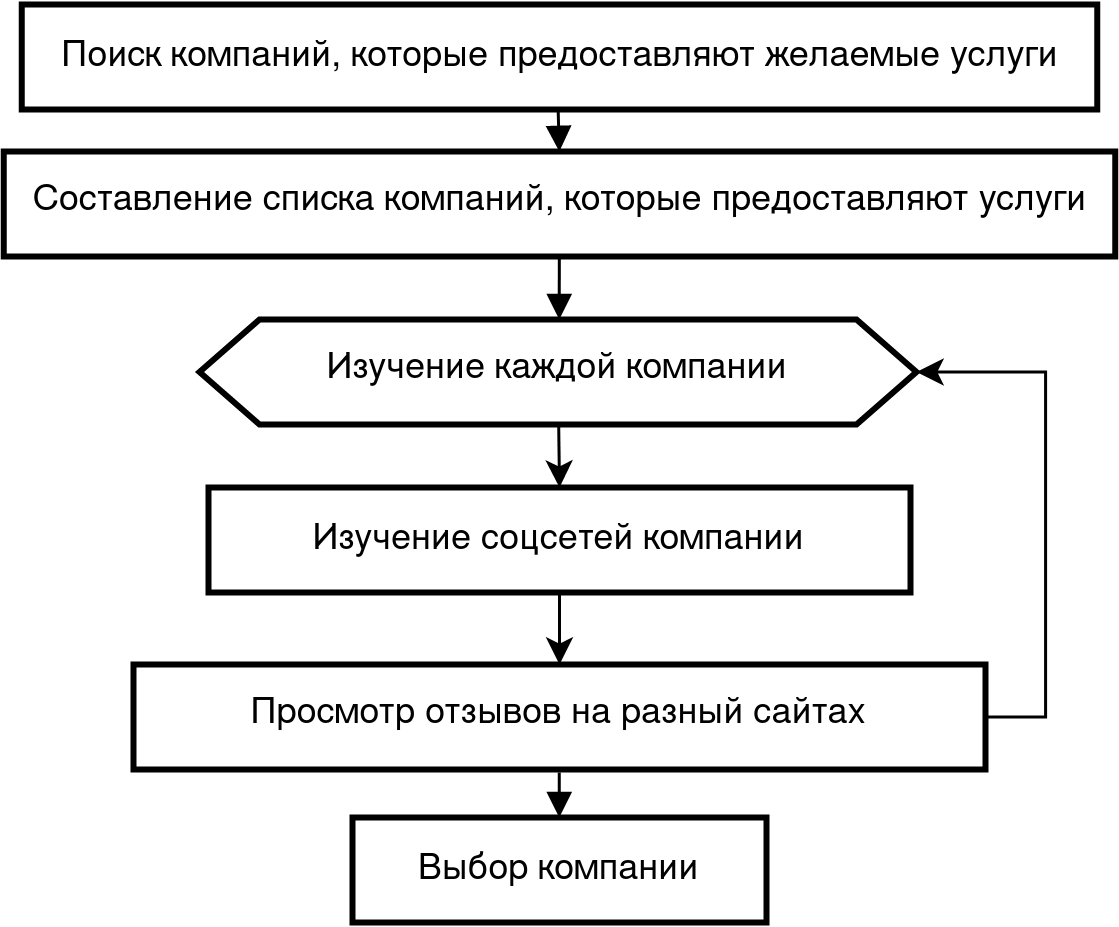
\includegraphics[width=0.6\textwidth]{img/mermaid/as_is_drawio.png}
\caption{\label{fig:as_is}Диаграмма того, как сейчас происходит поиск компании}
\end{figure}

\section{Анализ оценок этичности компаний}
\label{sec:org0d6ebb1}
Оценка этики компании -- это не одноразовый процесс, а скорее длительный и непрерывный процесс, который позволяет понять и оценить действия, политику и практику компании с течением времени. Оценка включает в себя рассмотрение соблюдения компанией отраслевых этических стандартов и передовой практики, а также мониторинг любых изменений в этической позиции компании с течением времени. Кроме того, участие в диалоге с компанией и консультации с организациями, специализирующимися на оценке корпоративной ответственности могут дать ценную информацию об этических практиках компании.

Компаниям важно оставаться этичными, так как в долгосрочной перспективе это приносит большую прибыль и улучшает показатели бизнеса, чем неэтичный способ ведение бизнеса\autocites{climent_ethical_2018}[][]{mure_esg_2021}. Насколько этична компания можно рассматривать с двух сторон, самой компании и их клиентов. Со стороны компаний можно выделить факторы, которые можно получить из их отчетности:
\begin{itemize}
\item размер капитала, чтобы они не могли обанкротиться.
\item влияние на окружающую среду.
\item куда идут инвестиции~\autocite{harvey_ethical_1995}.
\end{itemize}
Для пользователей одними из ключевых факторов можно выделить:
\begin{itemize}
\item качество пользовательского сервиса~\autocite{brunk_exploring_2010}, как правило пользователи оставляют отзывы на сайтах по пятибалльной шкале.
\item насколько навязчивы услуги компании~\autocite{mitchell_bank_1992}, как правило пользователи оставляют отзывы на сайтах по пятибалльной шкале.
\end{itemize}

В данной работе этичность компаний будет определяться по отзывам клиентов, которые могут в которых содержатся проблемы качества услуг и качество сервиса.
\section{Анализ существующих решений}
\label{sec:org9a83bbc}
Существует несколько индексов, предназначенных для измерения этичности -- индекс Dow Jones Sustainability Indices~(DJSI)~\autocite{lopez_sustainable_2007} и FTSE4GOOD~\autocite{collison_financial_2008}.

DJSI оценивает показатели устойчивости компаний различных секторов на основе экономических, экологических и социальных критериев. Компании отбираются на основе их показателей по сравнению с аналогичными компаниями в том же секторе. Процесс оценки включает в себя тщательную оценку компаний по различным критериям, включая корпоративное управление, экологический менеджмент, трудовую практику, права человека и социальные вопросы.

Аналогичным образом, индекс FTSE4GOOD предназначен для оценки деятельности компаний, которые демонстрируют эффективную практику экологического, социального и управленческого менеджмента (ESG). Компании отбираются на основе их практики ESG и оцениваются по различным критериям, включая изменение климата, права человека и корпоративное управление.

Индексы DJSI и FTSE4GOOD разработаны для того, чтобы помочь инвесторам определить компании, которые привержены этической практике. Эти индексы предоставляют инвесторам стандартизированный способ сравнения компаний на основе их показателей. Это помогает инвесторам принимать более обоснованные инвестиционные решения и побуждает компании внедрять устойчивую практику для привлечения инвестиций.

Для российских компаний нет аналогичных индексов. Сейчас данные об этичности компаний можно получить из агрегаторов отзывов и отчётности. Агрегаторы позволяют собрать информацию о клиентском обслуживании, а отчетность компаний о положении дел в целом. Но сейчас не существует способов, как можно оценить все вместе.
\section{Анализ требований к системе}
\label{sec:org900de53}
Исходя из интервью с заказчиком система должна уметь:

\begin{enumerate}
\item Показывать историю изменений индекса с возможностью фильтровать по:
\begin{enumerate}
\item Годам.
\item Отраслям компаний, с возможностью множественного выбора.
\item Компаниям, с возможностью множественного выбора.
\item Моделям, с возможностью множественного выбора.
\item Источникам, с возможностью множественного выбора.
\end{enumerate}
\item Агрегировать значения индекса по годам и кварталам.
\item Анализировать текстовые отзывы для построения индекса этичности на основании позитивности или негативности отзывов.
\item Иметь возможность добавления анализа текста несколькими вариантами.
\item Сохранять тексты для последующего анализа другими методами.
\item Система должна собирать данные с сайтов banki.ru, sravni.ru и комментарии из групп {}<<вконтаке>>{}.
\end{enumerate}

На основе описания функциональных требований была создана диаграмма вариантов использования, которая представлена на рисунке~\ref{fig:usecasefull}.
\begin{figure}[h!]
\centering
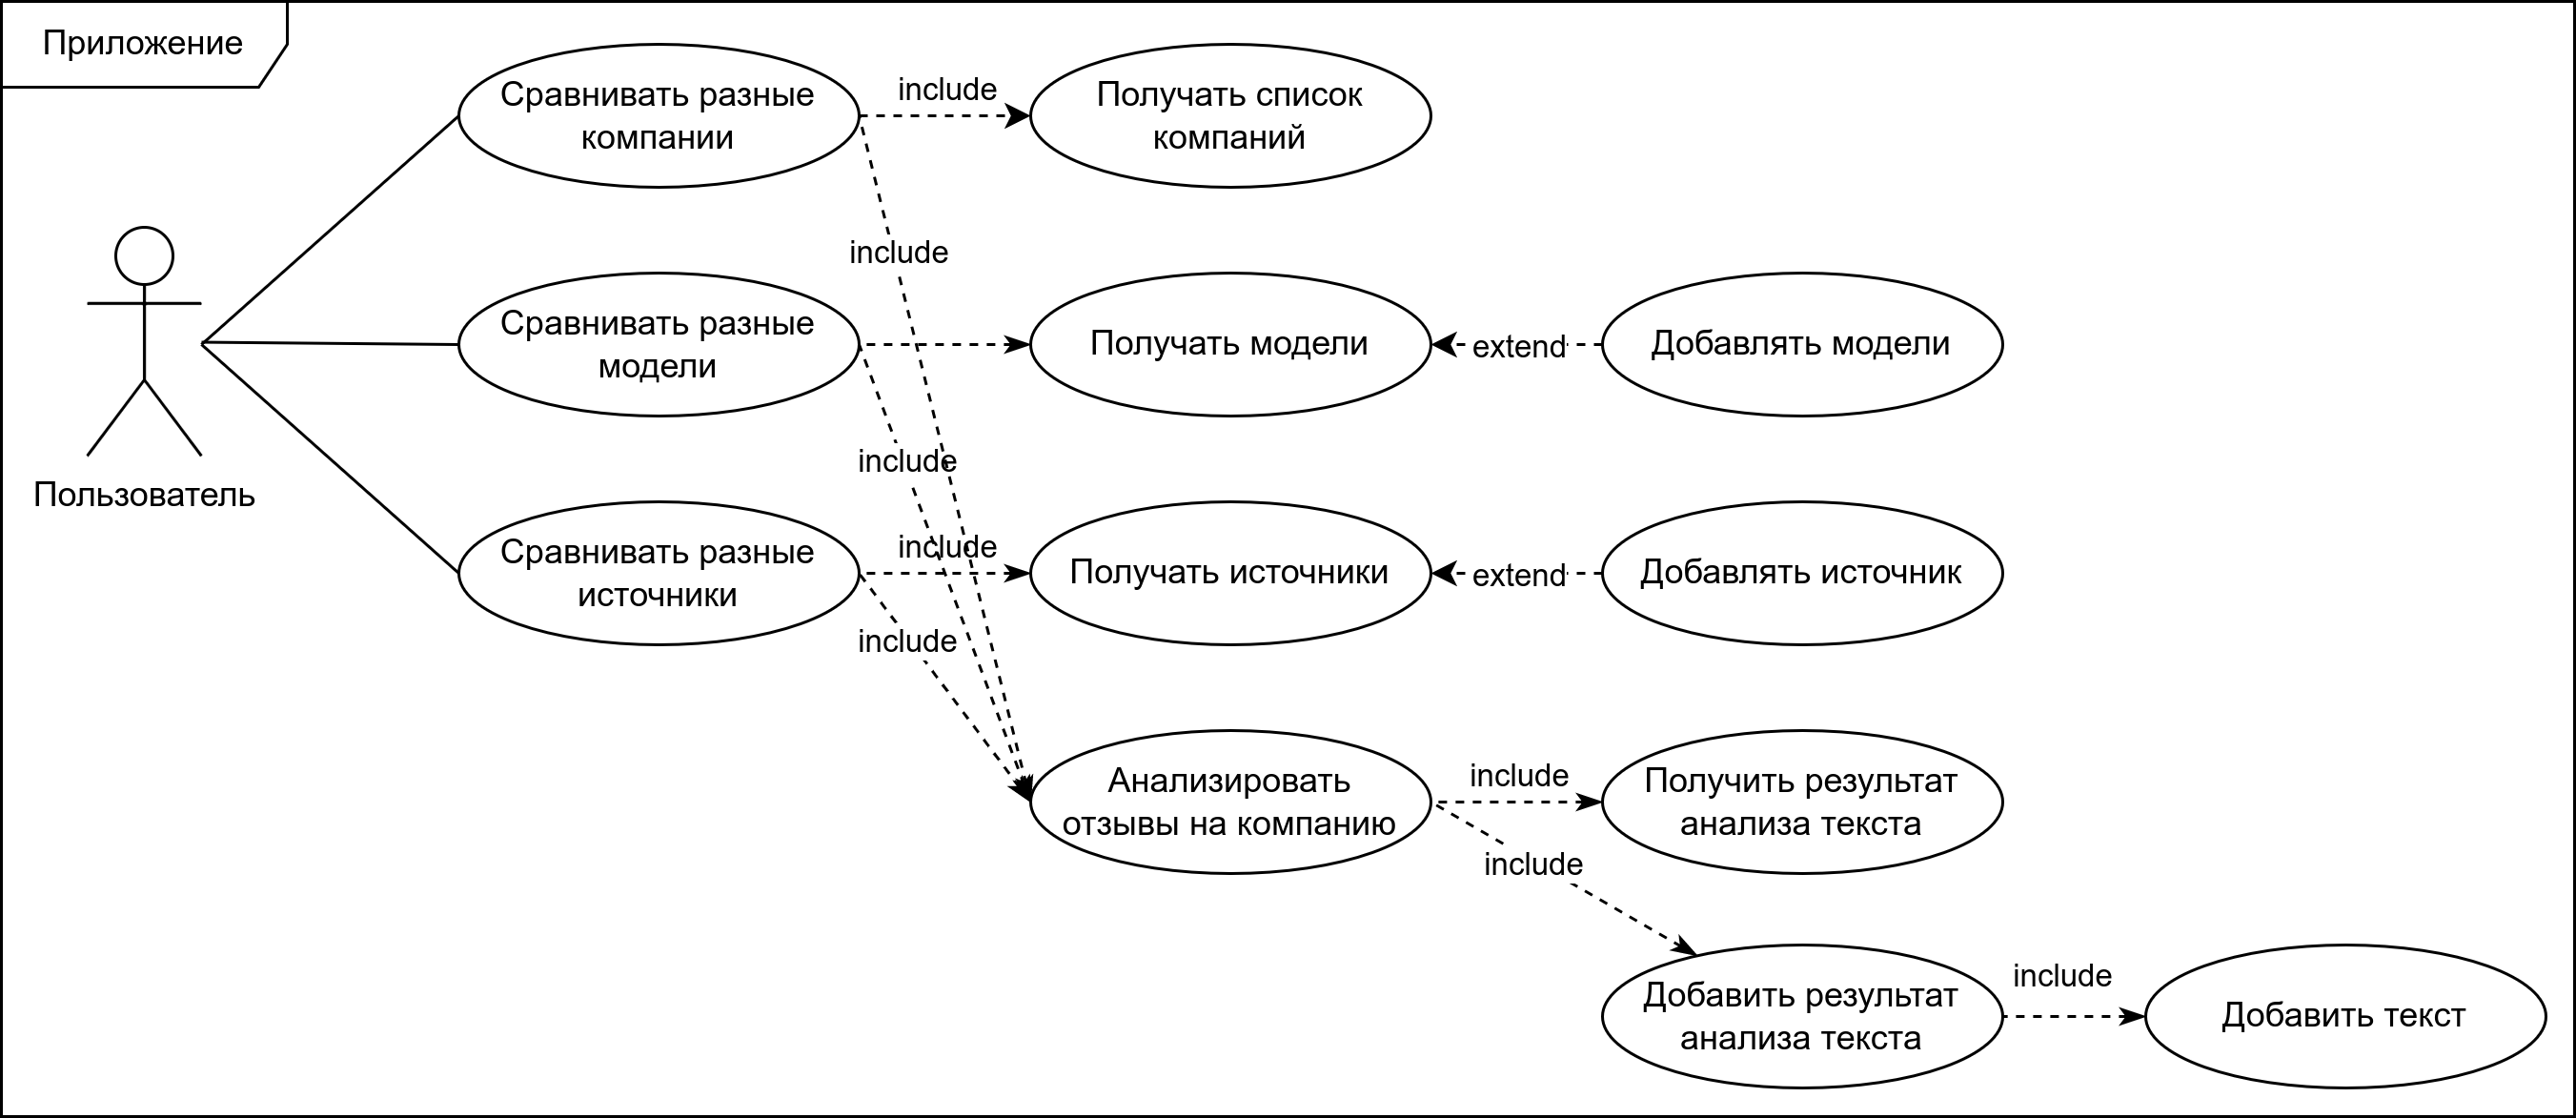
\includegraphics[width=\textwidth]{img/use-case.png}
\caption{\label{fig:usecasefull}Диаграмма вариантов использования}
\end{figure}

Также были получены нефункциональные требования:
\begin{enumerate}
\item Построение графика не должно занимать больше секунды.
\item Сбор данных должен происходить автоматически.
\item Данные должны обрабатываться автоматически.
\item Система должны способна работать с большим объемом информации. Несколько гигабайт текста.
\item Система должна быть стабильной и надежной, обеспечивая непрерывную работу без сбоев или перебоев.
\end{enumerate}
\section{Анализ метрик классификации}
\label{sec:org3ce147c}
Исходя из собранных требований в данной работе будет решаться задача классификации. Для определения качества работы алгоритма будут рассмотрены несколько метрик:
\begin{enumerate}
\item Доля правильных ответов
\item Точность
\item Полнота
\item F-мера
\end{enumerate}

Для лучшего понимания этих метрик рассмотрим матрицу ошибок. Матрица ошибок\ref{tbl:confusion_matrix} является таблицей, которая показывает количество верно и неверно классифицированных примеров для каждого класса. Она состоит из четырех значений:
\begin{itemize}
\item Истинно-положительные (True Positives, TP): количество примеров, которые были правильно классифицированы как положительные.
\item Истинно-отрицательные (True Negatives, TN): количество примеров, которые были правильно классифицированы как отрицательные.
\item Ложно-положительные (False Positives, FP): количество примеров, которые были неправильно классифицированы как положительные.
\item Ложно-отрицательные (False Negatives, FN): количество примеров, которые были неправильно классифицированы как отрицательные.
\end{itemize}

\begin{table}[h!]
\caption{\label{tbl:confusion_matrix}Матрица ошибок}
\centering
\begin{tabular}{|c|c|c|}
\hline
 & y=1 & y=0\\[0pt]
\hline
f(x)=1 & True Positives, TP & False Positives, FP\\[0pt]
\hline
f(x)=0 & False Negatives, FN & True Negatives, TN\\[0pt]
\hline
\end{tabular}
\end{table}

Доля правильных \ref{eq:accuracy} ответов (Accuracy) показывает, как часто модель правильно классифицирует примеры. Она вычисляется как отношение числа верно классифицированных примеров к общему числу примеров:

\begin{equation}
\label{eq:accuracy}
\text{{Accuracy}} = \frac{{TP + TN}}{{TP + TN + FP + FN}}
\end{equation}

Точность \ref{eq:precision} (Precision) показывает, какая доля примеров, классифицированных как положительные, действительно является положительными. Она вычисляется как отношение числа истинно-положительных примеров к сумме истинно-положительных и ложно-положительных примеров:

\begin{equation}
\label{eq:precision}
\text{{Precision}} = \frac{{TP}}{{TP + FP}}
\end{equation}

Полнота \ref{eq:recall} (Recall) показывает, какая доля положительных примеров была правильно классифицирована. Она вычисляется как отношение числа истинно-положительных примеров к сумме истинно-положительных и ложно-отрицательных примеров:

\begin{equation}
\label{eq:recall}
  \text{{Recall}} = \frac{{TP}}{{TP + FN}}
\end{equation}

F-мера \ref{eq:f1_score} (F1 Score) является гармоническим средним между точностью и полнотой. Она позволяет учесть оба показателя и оценить баланс между ними. Лучше всего подходит для несбалансированных выборок. F-мера вычисляется по формуле:
\begin{equation}
\label{eq:f1_score}
F1 = 2 \times \frac{{\text{{Precision}} \times \text{{Recall}}}}{{\text{{Precision}} + \text{{Recall}}}}
\end{equation}

Выбор метрики для определения качества работы алгоритма будет зависеть от данных для ее обучения.
\section{Алгоритмы для обработки естественного языка}
\label{sec:org7113e2e}
В требованиях было заявлено, что для оценки этичности компаний надо обрабатывать текстовые отзывы, поэтому в данной работе будут рассмотрены алгоритмы по обработке естественного языка.

Алгоритмы машинного обучения для анализа текста получили широкое распространение для извлечения информации из неструктурированных данных с помощью больших помеченных наборов данных. Среди различных используемых методов несколько алгоритмов оказались особенно эффективными в этой области. Каждый из этих алгоритмов обладает уникальными характеристиками, которые делают их хорошо подходящими для определенных задач. В этом разделе будут рассмотрены следующие алгоритмы:
\begin{enumerate}
\item Мешок слов
\item TF-IDF
\item Word2Vec
\item FastText
\item BERT
\end{enumerate}
\subsection{Мешок слов}
\label{sec:orga479ea2}
Мешок слов~\autocite{harris_distributional_1954} -- метод анализа, который позволяет упрощенно представить текст, как таблицу, где для каждого документа показано количество вхождений слова. В данной модели все слова предстают как множество слов без учёта грамматики и порядка. В процессе обработки текст разбивается на отдельные слова или токены, игнорируя грамматические правила и порядок слов. Затем строится словарь, содержащий все уникальные слова из текстового корпуса. Каждому слову в словаре присваивается уникальный идентификатор. После построения словаря каждый документ представляется в виде вектора, где каждый элемент вектора соответствует слову из словаря, а значение элемента -- количество вхождений этого слова в документе. Таким образом, каждый документ представляется в виде разреженного вектора, где большинство элементов равно нулю. Например, для предложений «Мама мыла раму»(1) и «Иван поломал раму»(2) результат работы алгоритма показан в таблице \ref{tbl:bow}:
\begin{table}[htbp]
\caption{\label{tbl:bow}Пример мешка слов}
\centering
\begin{tabular}{|c|c|c|c|c|c|}
\hline
 & мама & мыла & раму & иван & поломал\\[0pt]
\hline
текст1 & 1 & 1 & 1 & 0 & 0\\[0pt]
\hline
текст2 & 0 & 0 & 1 & 1 & 1\\[0pt]
\hline
\end{tabular}
\end{table}
\subsection{TF-IDF}
\label{sec:org69d76aa}
TF-IDF~\autocite{joneskarensparck_statistical_1972} (TF частотность слова (term frequency), IDF -- обратная частота документов (inverse document frequency)) -- статистический показатель, применяемый для оценки важности слова в контексте документа. Большой вес в TF-IDF получат слова с высокой частотой в пределах конкретного документа и с низкой частотой употреблений в других документах. В процессе TF-IDF текст разбивается на отдельные слова или токены, игнорируя грамматические правила и порядок слов.

TF -- частота слова в коллекции. Таким образом, оценивается важность слова \(t_{i}\) по формуле~\ref{eq:tf}:

\begin{equation}
\label{eq:tf}
TF(t,d)=\frac{n_{t}}{\sum_{k}n_{k}},
\end{equation}
где \(n_{t}\) -- число вхождений слова \(t\) в документ, а в знаменателе -- общее число слов в данном документе.

IDF -- инверсия частоты, с которой некоторое слово встречается в документах коллекции. Чем реже слово встречается в документах, тем выше значение IDF и тем больше важности придается слову в контексте корпуса. Оно рассчитывается по формуле~\ref{eq:IDF}.

\begin{equation}
\label{eq:IDF}
IDF(t, D)=\log\frac{|D|}{|\{d_{i}\in D\mid t \in d_{i}\}|},
\end{equation}
где \(|D|\) -- число документов в коллекции, а \(|{d_{i}\in D|t\in d_{i}}|\) -- число документов из коллекции \(D\), в которых встречается \(t\) (когда \(n_{t}\neq 0\)).

Таким образом, мера TF-IDF является произведением двух множителей~\ref{eq:TFIDF}:
\begin{equation}
\label{eq:TFIDF}
\text{TF-IDF}(t,d,D)=TF(t,d)\times IDF(t,d)
\end{equation}
\subsection{Word2Vec}
\label{sec:org21d8af1}
Word2Vec~\autocite{mikolov_distributed_2013} -- это алгоритм обработки естественного языка, который используется для получения векторных представлений (эмбеддингов) слов на основе их семантического контекста. Он работает на основе распределенного представления слов, идея которого состоит в том, что слова, встречающиеся в похожих контекстах, имеют схожие семантические значения. Алгоритм предлагает две основные архитектуры: CBOW (непрерывный мешок слов) и Skip-gram.

\begin{enumerate}
\item Непрерывный мешок слов:
Архитектура CBOW состоит в обучении модели для предсказания целевого слова на основе контекстных слов. Например, для предложения {}<<Мама мыла раму>>{} модель CBOW пытается предсказать слово {}<<мыла>>{} на основе остальных слов.
\item Skip-gram:
Архитектура Skip-gram работает в обратном направлении по сравнению с CBOW. Она предсказывает контекстные слова на основе целевого слова. То есть для слова {}<<мыла>>{} модель Skip-gram пытается предсказать остальные контекстные слова.
\end{enumerate}

Результатом обучения Word2Vec являются векторные представления слов, где каждое слово представлено вектором фиксированной длины. Векторы слов сохраняют в себе семантическую информацию о значениях слов и их семантической близости.
\subsection{FastText}
\label{sec:org734ba7f}
FastText~\autocite{joulin_bag_2016}- это библиотека и метод машинного обучения, разработанный командой Facebook AI Research, для обработки естественного языка. Он является эффективным инструментом для работы с текстовыми данными и создания векторных представлений слов.

FastText расширяет идею Word2Vec, добавляя поддержку для обработки подслов. В отличие от Word2Vec, который работает только на уровне слов, FastText представляет слова как комбинации символьных n-грамм. N-граммы - это последовательности символов фиксированной длины, которые могут быть префиксами, суффиксами или внутренними частями слова.
\subsection{BERT}
\label{sec:orgce3e872}
BERT~\autocite{devlin_bert_2019} (Bidirectional Encoder Representations from Transformers) -- это нейросетевая языковая модель, которая относится к классу трансформеров. Она состоит из 12 «базовых блоков» (слоев), а на каждом слое 768 параметров.

На вход модели подается предложение или пара предложений. Затем разделяется на отдельные слова (токены). Потом в начало последовательности токенов вставляется специальный токен \texttt{[CLS]}, обозначающий начало предложения или начало последовательности предложений. Пары предложений группируются в одну последовательность и разделяются с помощью специального токена \texttt{[SEP]}, затем к каждому токену добавляется эмбеддинг, показывающий к какому предложению относится токен. Потом все токены превращаются в эмбеддинги~\ref{fig:inputemebeddings} по механизму описанному в работе~\autocite{vaswani_attention_2017}.

\begin{figure}[h]
\centering
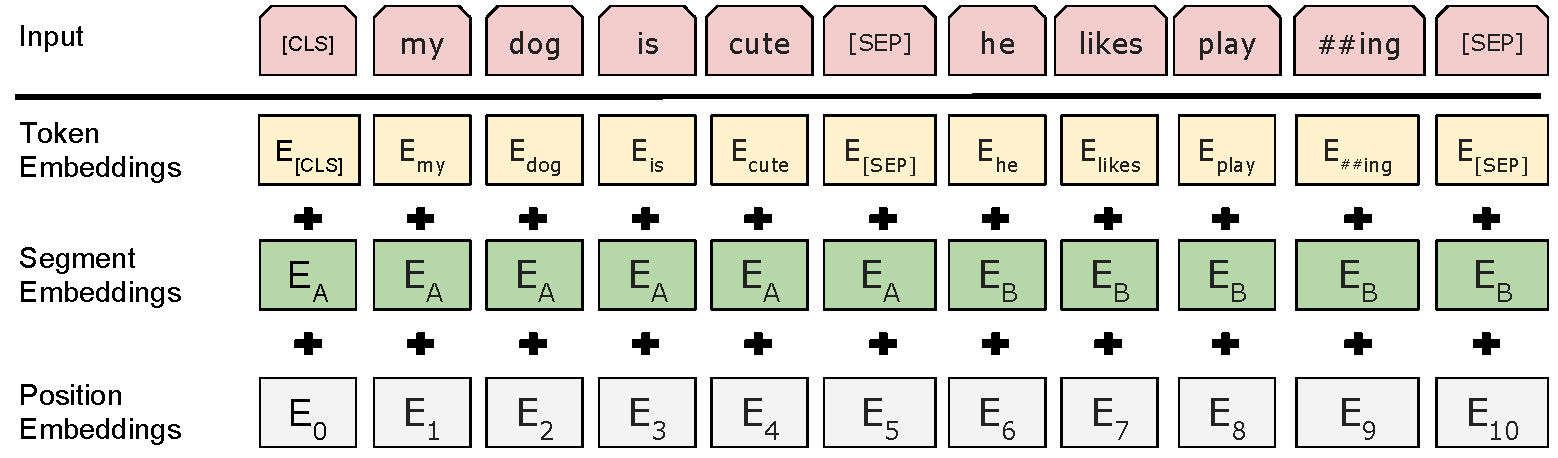
\includegraphics[width=.9\linewidth]{img/Input_Emebeddings.pdf}
\caption{\label{fig:inputemebeddings}Пример ввода текста в модель}
\end{figure}

При обучении модель выполняет на 2 задания:
\begin{enumerate}
\item Предсказание слова в предложении

Это задание обучается следующим образом -- 15\% случайных слов заменяются в каждом предложении на специальный токен \texttt{[MASK]}, а затем предсказываются на основании контекста. Однако иногда слова заменяются не на специальны токена, в 10\% заменяются на случайный токен и еще в 10\% заменяются на случайное слово.

Поскольку стандартные языковые модели~\ref{fig:BERT_comparisons}, такие как ELMo~\autocite{peters_deep_2018} и GPT~\autocite{radford_language_2019}, либо смотрят текст слева направо, либо справа налево, они не подходят для некоторых типов заданий. Однако BERT является двунаправленной моделью, что означает, что для каждого слова он может рассмотреть его контекст и использовать эту информацию для предсказания замаскированного слова.

\begin{figure}[h]
\centering
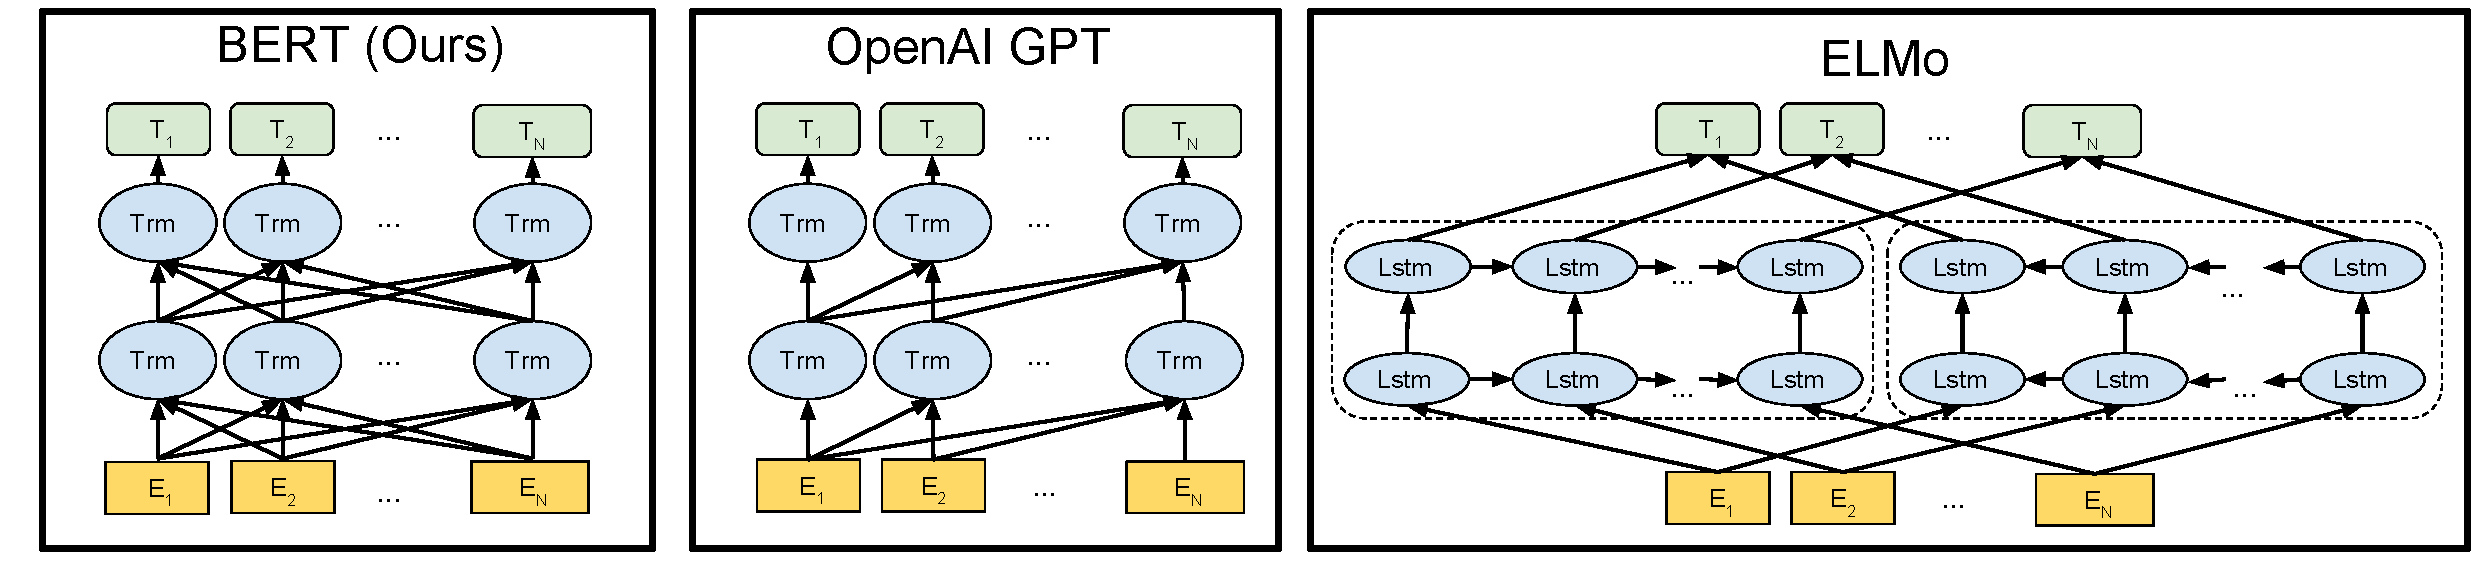
\includegraphics[width=.9\linewidth]{img/BERT_comparisons.pdf}
\caption{\label{fig:BERT_comparisons}Сравнение принципов работы BERT, ELMo, GPT}
\end{figure}
\item Предсказание следующего предложения

Для того чтобы обучить модель, которая понимает отношения предложений, она предсказывает, идут ли предложения друг за другом. Для этого с 50\% вероятностью выбирают предложения, которые находятся рядом и наоборот. Пример ввода пары предложений в модель~\ref{fig:bert_pretrainin}.

\begin{figure}[h]
\centering
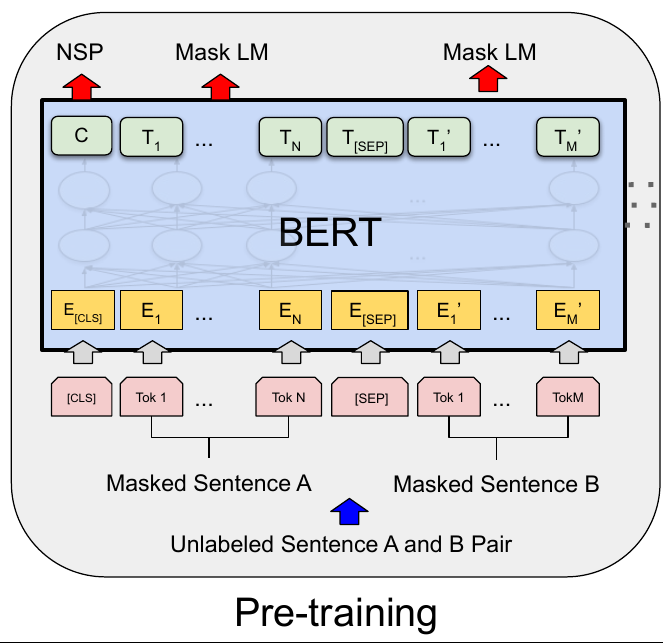
\includegraphics[width=0.6\textwidth]{img/bert_pretrainin.png}
\caption{\label{fig:bert_pretrainin}Схемам работы BERT}
\end{figure}
\end{enumerate}
\subsection{Выводы}
\label{sec:orgeefd61a}
В данном разделе были рассмотрены различные алгоритмы для обработки текста. Как показали исследования\autocite{gonzalez-carvajal_comparing_}, каждый алгоритм может подойти к той или иной задаче, поэтому в данной работе они все будут рассмотрены.
\section{Алгоритмы для классификации}
\label{sec:org0072ce5}
Для определения на сколько этична компания, каждый отзыв будет классифицироваться. Для этого будут рассмотрены следующие алгоритмы:
\begin{enumerate}
\item Логическая регрессия
\item Метод опорных векторов
\item Случайный лес
\item Градиентный бустинг
\end{enumerate}
\subsection{Логистическая регрессия}
\label{sec:org1078411}
Логистическая регрессия\autocite{fan_liblinear_2008} является одним из наиболее распространенных алгоритмов машинного обучения, который применяется для задач классификации. Она основана на логистической функции~\ref{eq:logreg}, которая преобразует входные данные в вероятности принадлежности к определенным классам.

\begin{equation}
\label{eq:logreg}
f(z)=\frac{1}{1+\exp(-z)},
\end{equation}
где z -- скалярное произведение весов модели, на признаки ответа.
\subsection{Метод опорных векторов}
\label{sec:org7053629}
Метод опорных векторов\autocite{platt_probabilistic_2000} (Support Vector Machine, SVM) — это алгоритм машинного обучения, который используется для задач классификации и регрессии. Он основан на принципе максимизации зазора (margin) между классами объектов.

Идея SVM заключается в том, чтобы найти оптимальную гиперплоскость, которая разделяет два класса объектов в максимально возможном зазоре. Гиперплоскость представляет собой (n-1)-мерную гиперплоскость в n-мерном пространстве, где n - количество признаков.

Данная модель часто применяется для текстовой классификации\autocite{joachims_text_1998}.
\subsection{Случайный лес}
\label{sec:org68d02c6}
Случайный лес\autocite{breiman_random_2001}(Random Forest) является ансамблевым методом машинного обучения, который объединяет несколько решающих деревьев для решения задач классификации и регрессии. Каждое дерево строится независимо от других на основе различных подвыборок данных (bootstrap samples) и случайного подмножества признаков. Это позволяет деревьям быть разнообразными и уменьшает корреляцию между ними. На каждом узле дерева выбирается лучший признак и значение порога, на которое данные будут разделены на две ветви. Этот выбор делается на основе критерия информативности, такого как индекс Джини (для классификации) или среднеквадратичная ошибка (для регрессии).
\subsection{Boosting}
\label{sec:orgd494053}
Градиентный бустинг\autocite{friedman_greedy_2001} (Gradient Boosting) - это алгоритм машинного обучения, который также является ансамблевым методом, но в отличие от случайного леса, градиентный бустинг строит ансамбль слабых моделей (обычно решающих деревьев) последовательно, обучая каждую модель на ошибках предыдущих моделей.

Сначала инициализируется начальная модель, которая может быть простой, например, константой или средним значением целевой переменной. Это начальное предсказание будет постепенно улучшаться в процессе построения ансамбля моделей. Затем строится первая модель. Ошибка между предсказанными значениями первой модели и фактическими значениями вычисляется с помощью функции потерь, такой как среднеквадратичная ошибка (для задач регрессии) или логистическая функция потерь (для задач классификации). После обучения первой модели вычисляется градиент функции потерь по отношению к предсказаниям первой модели. Градиент показывает, в каком направлении и насколько сильно нужно скорректировать предсказания первой модели, чтобы уменьшить ошибку.  Далее строится следующая модель, которая обучается на остатках первой модели. Остатки представляют собой разницу между фактическими значениями и предсказаниями первой модели. Вторая модель приближает остатки, чтобы улучшить предсказания

Одни из самых популярных реализаций градиентного бустинга:
\begin{enumerate}
\item Scikit-learn -- эта реализация предлагает простую реализации градиентного бустинга с удобным интерфейсом.
\item XGBoost\autocite{chen_xgboost_2016} -- предоставляет много дополнительных возможностей и оптимизаций, которые делают ее одной из наиболее мощных библиотек для градиентного бустинга. Обладает высокой производительностью и позволяет обучаться на GPU\autocite{mitchell_accelerating_2017}, что ускоряет процесс.
\item CatBoost\autocite{prokhorenkova_catboost_2018} -- относительно новой библиотекой градиентного бустинга, разработанной компанией Yandex. Он имеет сходные функции и возможности с XGBoost, но также включает в себя некоторые уникальные возможности, которые лучше позволяют обрабатывать параметры, которые отвечают за категориальные признаки. Также имеет поддержку обучения на GPU\autocite{dorogush_catboost_2018}.
\end{enumerate}
\subsection{Выводы}
\label{sec:org4522e30}
Все рассмотренные алгоритмы часто используется для анализа текста и не ясно, какой из них справится лучше в поставленной задаче. Поэтому в данной работе будут рассмотрены все эти алгоритмы.
\section{Выбор технологий для разработки}
\label{sec:org41c58eb}
Для реализации этой системы будет использоваться язык Python\autocite{vanrossum_python_2009}. Для этого языка разработано много библиотек, которые позволят быстро реализовать алгоритмы обработки естественного языка, в частности в этом проекте будет использоваться Pytorch~\autocite{paszke_pytorch_2019} и HuggingFace~\autocite{wolf_transformers_2020}. Для реализации API будет использоваться FastAPI, что позволит разработать API для системы с автоматической генерацией документации.

Для хранения данных будет использоваться объектно-реляционная система управления базами данных PostgreSQL, что позволит обрабатывать большие объемы данных. Для работы с ней будет использоваться Code first подход, с помощью Python библиотек Sqlalchemy и Alembic для изменения схемы данных (миграций).
\section{Выводы по главе}
\label{sec:org17aeca2}
По итогам анализа предметной области, можно сделать вывод о том, что определение этичности компаний является важной задачей, так как с ней сталкиваются многие люди ежедневно и тратят много времени, которую можно автоматизировать с помощью алгоритмов машинного обучения. Обзор существующих решений показал, что сейчас нет индекса, который бы учитывал мнение клиентов для анализа этичности, и может потребоваться разработка нового средства, учитывающего особенности задачи.

Изучение существующих исследований и работ показало, что в сфере обработки естественного языка применяются мешок слов, TF-IDF, Word2Vec, FastText и BERT и каждый из этих алгоритмов показал свою эффективность.

Также для задач классификации были рассмотрены: логистическая регрессия, метод опорных векторов, случайный лес и градиентный бустинг. И они будут рассмотрены в этой работе.

Анализ требований к системе позволяет определить необходимые функциональные и нефункциональные требования, которые будут учитываться при разработке решения. Исходя из полученной информации, было разработано техническое задание~\ref{tz_chap}.
\chapter{Проектирование системы}
\label{sec:org6ace4b2}
В данной главе представлена общая архитектура системы, базы данных и каждого модуля отдельно.

Этап проектирования следует разделить на следующие пункты:
\begin{enumerate}
\item Определение основных компонентов приложения и проектирование архитектуры системы.
\item Проектирование базы данных и модулей для работы, обработки, сбора и агрегации данных.
\item Проектирование модели для обработки естественного текста.
\end{enumerate}

Данная глава предоставляет описание системы, каждого компонента и их взаимосвязь в достижении желаемого результата.
\section{Создание метода для оценки этичности}
\label{sec:orgf15aaa5}
Для оценки этичности компаний в данном исследовании принимается во внимание отзывы, оставленные о них, и анализируется их характер - позитивный или негативный. Изначально использовался подход, основанный на разности долей позитивных и негативных отзывов (базовый индекс, Base index). Этот метод эффективен при большом количестве отзывов, однако при небольшом объеме отзывов он не предоставляет достоверную картину.

Поскольку люди склонны писать отзывы чаще о негативном опыте, чем о положительном, среднее значение индекса обычно имеет отрицательное значение. Это нежелательно с точки зрения оценки этичности компаний. С целью преодолеть этот эффект, рассчитывается среднее значение - разность позитивных и негативных долей отзывов за год для каждого источника компании (средний индекс, Mean Index). Затем это значение вычитается из базового индекса, что приближает его к нулю. В результате компании с средним уровнем этичности будут иметь значение индекса около нуля, тогда как компании, которые проявляют более низкий или высокий уровень этичности, будут иметь отрицательное или положительное значение соответственно.

Данный подход эффективен при наличии большого числа отзывов, однако при ограниченном количестве отзывов значение индекса может быть слишком велико или слишком мало, не отражая действительное качество компаний. Для учета этого смещения было решено использовать доверительные интервалы.

Поскольку позитивность и негативность отзыва это дискретная величина, то она будет иметь распределение Бернулли\autocite{_encyclopaedia_}. Дисперсия этого распределения рассчитывается по формуле \(pq\) для одной точки, а для последовательность \(\frac{pq}{n}\), где \(p\) вероятность 1, и \(q\) вероятность 0. В данной задаче \(p\) будет рассчитываться, как доля класса среди всех отзывов, а \(q\) как доля остальных отзывов.

В конечном итоге для вычисления индекса средней компании используется абсолютная разность между базовым индексом и средним индексом, а затем из этого значения вычитается дисперсия (полученная формула \ref{eq:ethics}). Это приводит к тому, что компании с ограниченным количеством отзывов имеют большое стандартное отклонение, что означает, что их индекс будет близок к нулю или точно равен нулю. С другой стороны, у компаний с большим количеством отзывов стандартное отклонение будет меньшим, и оно либо не изменит, либо незначительно изменит их значение индекса. Таким образом, этот метод позволяет проверить, пересекается ли доверительный интервал индекса с нулевым значением. Если интервал пересекается, это означает, что значение индекса близко к нулю, а если интервал не пересекается, то берется консервативная нижняя оценка. Такой подход к вычислению индекса делает его более нейтральным и менее подверженным выбросам.

\begin{equation}
\label{eq:ethics}
\begin{aligned}
    \text{Base index} &= \frac{\text{positive} - \text{negative}}{\text{total}} \\
    \text{Std index} &= \sqrt{\frac{\text{positive}\cdot(\text{total-positive})}{total^{3}} + \frac{\text{negative}\cdot(\text{total - neutral})}{total^{3}}} \\
    \text{Index} &=
        \begin{cases}
            \max(\text{Base Index}-\text{Mean Index}-\text{Std Index},0), & \text{Base index} > \text{Mean index} \\
            \min(\text{Base Index}-\text{Mean Index}+\text{Std Index},0), & \text{Base index} < \text{Mean index} \\
        \end{cases}
% (2 * ((index_base - index_mean) > 0) - 1) * (max(abs(index_base - index_mean) - index_std, 0))
\end{aligned}
\end{equation}


\(positive\) -- количество позитивных предложений,

\(negative\) -- количество негативных предложений,

\(total\) -- количество предложений.
\section{Проектирование определения наиболее подходящей модели}
\label{sec:org5f307f3}
Для определения наиболее подходящей модели будет использоваться набор данных, состоящий из 6,000 предложений, размеченных тремя экспертами с учетом этических практик. Однако классы предложений в этом наборе данных оказались несбалансированными, как показано на диаграмме~\ref{fig:class_balance} (с отрицательными предложениями, обозначенными {}<<->>{}, в большем количестве, чем положительными предложениями, обозначенными {}<<+>>{}). Поэтому в качестве основной метрики будет использоваться F1-мера, так как она наиболее подходит для работы с несбалансированными наборами данных. Для улучшения работы алгоритмов для определения класса каждого предложения будет использоваться наиболее часто встречающийся класс, назначенный экспертами.

\begin{figure}[h!]
\centering
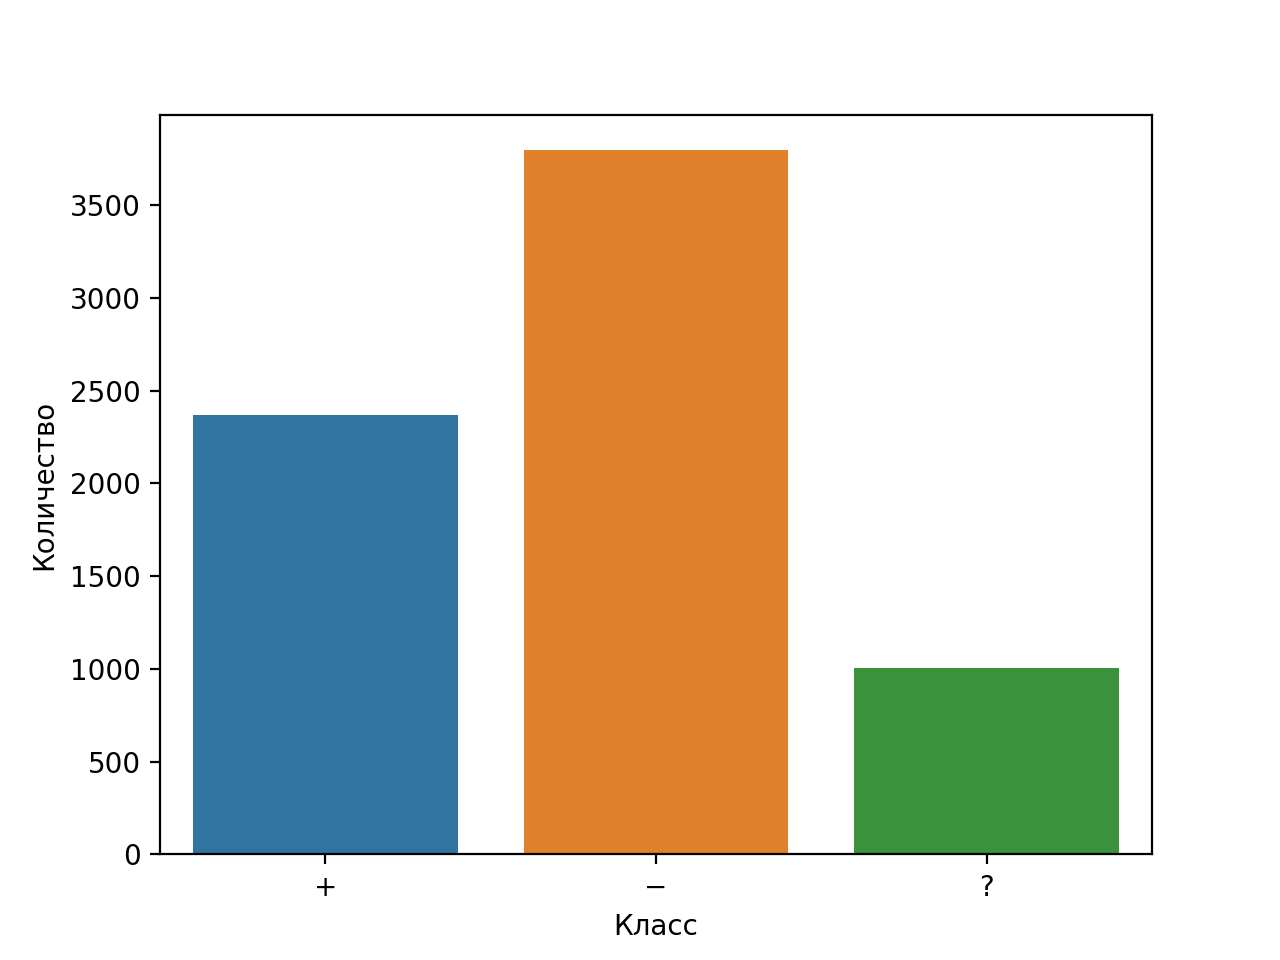
\includegraphics[width=0.8\textwidth]{img/class_balance.png}
\caption{\label{fig:class_balance}Распределение классов}
\end{figure}

Для обработки текста будут рассмотрены алгоритмы, результат работы которых будет подаваться на вход алгоритму кластеризации:
\begin{enumerate}
\item Мешок слов.
\item TF-IDF.
\item Word2Vec обученный на русском языке.
\item fastText обученный на русском языке~\autocite{korogodina_evaluation_2020}.
\item Модификация BERT для русского языка RuBERT~\autocite{kuratov_adaptation_2019}.
\item RuBERT дообученый на классификацию эмоций.
\item Дообученый RuBERT на собранных данных.
\end{enumerate}

Перед подачей в модели данные отзывы будут предварительно очищены от цифр и ссылок, а также произведено их приведение к начальной форме (лемматизация). Для моделей, основанных на BERT, отзывы будут обрабатываться в двух вариантах: исходный текст и текст, подвергнутый обработкам.

Для определения наиболее подходящего алгоритма определения этичности будут перебираться все пары метода обработки текста и моделей для классификации. Для каждого алгоритма классификации будут подобраны оптимальные параметры, которые позволят сделать наилучшее предсказание на данных.

Для логистической регрессии будут подобраны следующие параметры:
\begin{enumerate}
\item С -- параметр отвечающий за силу регуляризации алгоритма. Будет подбираться от 0.00001 до 100.
\item Penalty -- параметр отвечающий за тип регуляризации l1 или l2.
\item Solver -- тип алгоритма оптимизации libliniar\autocite{fan_liblinear_2008} или saga\autocite{defazio_saga_2014}.
\item Max\_iter-- количество итераций для обучения. Будет подбираться от 100 до 1000.
\end{enumerate}

Для метода опорных векторов будут подобраны следующие параметры:
\begin{enumerate}
\item С -- параметр отвечающий за силу регуляризации алгоритма. Будет подбираться от 0.00001 до 100.
\item Kernel -- тип ядра для SVM (linear, poly, rbf или sigmoid).
\item Gamma -- коэффициент ядра (scale или auto).
\item Degree -- степень полиномиального ядра. Будет подбираться от 1 до 5
\end{enumerate}

Для случайного леса будут подобраны следующие параметры:
\begin{enumerate}
\item N\_estimators -- количество итераций для обучения. Будет подбираться от 100 до 1000.
\item Max\_depth -- глубина дерева. Будет подбираться от 1 до 10.
\item Max\_features -- количество признаков для разбиения на каждом узле (корень из количества параметров или логарифм по основанию 2).
\item Criterion -- критерий для разбиения узлов дерева (Джини или кросс-энтропия).
\end{enumerate}

Для градиентного бустинга (scikit-learn) будут подобраны следующие параметры:
\begin{enumerate}
\item Learning\_rate -- сколько вносит каждое дерево в алгоритм. Будет подбираться от 0.00001 до 1.
\item N\_estimators -- количество итераций для обучения. Будет подбираться от 100 до 1000.
\item Max\_depth -- глубина дерева. Будет подбираться от 1 до 10.
\item Max\_features -- количество признаков для разбиения на каждом узле (корень из количества параметров или логарифм по основанию 2).
\end{enumerate}

Для xgboost будут подобраны следующие параметры:
\begin{enumerate}
\item N\_estimators -- количество итераций для обучения. Будет подбираться от 100 до 1000.
\item Max\_depth -- глубина дерева. Будет подбираться от 1 до 10.
\item Learning\_rate -- сколько вносит каждое дерево в алгоритм. Будет подбираться от 0.00001 до 1.
\item Gamma -- минимальное уменьшение функции потерь, необходимое для создания нового разбиения на узле. Будет подбираться от 0 до 20.
\item Subsample -- доля обучающих примеров, используемых для обучения каждого дерева. Будет подбираться от 0 до 1.
\end{enumerate}

Для catboost будут подобраны следующие параметры:
\begin{enumerate}
\item N\_estimators -- количество итераций для обучения. Будет подбираться от 100 до 1000.
\item Max\_depth -- глубина дерева. Будет подбираться от 1 до 10.
\item Learning\_rate -- сколько вносит каждое дерево в алгоритм. Будет подбираться от 0.00001 до 1.
\end{enumerate}

Потом результаты работы каждого алгоритма с лучшими гиперпараметрами будут сравниваться между друг другом по F1 и так определиться лучшая модель.
\section{Проектирование архитектуры системы}
\label{sec:org4a62bd5}
Система будет разделена на отдельные независимые компоненты (микросервисы), что позволит ей быть надежной (если в какой-то части системы будут сбои, то остальная часть системы продолжит работать) и масштабируемой (легко добавлять новые компоненты). Каждый микросервис системы будет представлять собой docker container\autocite{merkel_docker_2014}, который будет управляться с помощью docker compose. Каждый сервис будет реализовывать отдельный компонент бизнес-логики и взаимодействовать с другими компонентами через REST API.

Было выделено 4 главных компонента бизнес логики:
\begin{enumerate}
\item Работа с базой данных -- это HTTP API, который обеспечивает возможность сохранения и получения данных из базы данных. Данный компонент принимает запросы на сохранение данных, получение информации из базы данных и возвращает результаты обработки этих запросов.
\item Сбор данных -- компонент, который отвечает за сбор информации с нескольких источников. Для этого используется несколько независимых сборщиков данных, которые работают с различными сайтами и другими источниками.
\item Обработка данных -- данный компонент содержит несколько моделей, которые используются для анализа данных. Эти модели производят различные виды анализа, от простой фильтрации и сортировки до более сложных операций анализа и прогнозирования.
\item Агрегирование данных -- этот компонент отвечает за агрегацию обработанных данных в единый индекс. Данный индекс может быть использован для удобного представления полученных результатов в виде отчетов и графиков. Данный модуль нужен для того чтобы быстро получать новые графики, так как агрегирование всех отзывов для компаний может занимать много времени.
\end{enumerate}

Результат архитектуры системы на рис.~\ref{fig:architecture}.

\begin{figure}[h!]
\centering
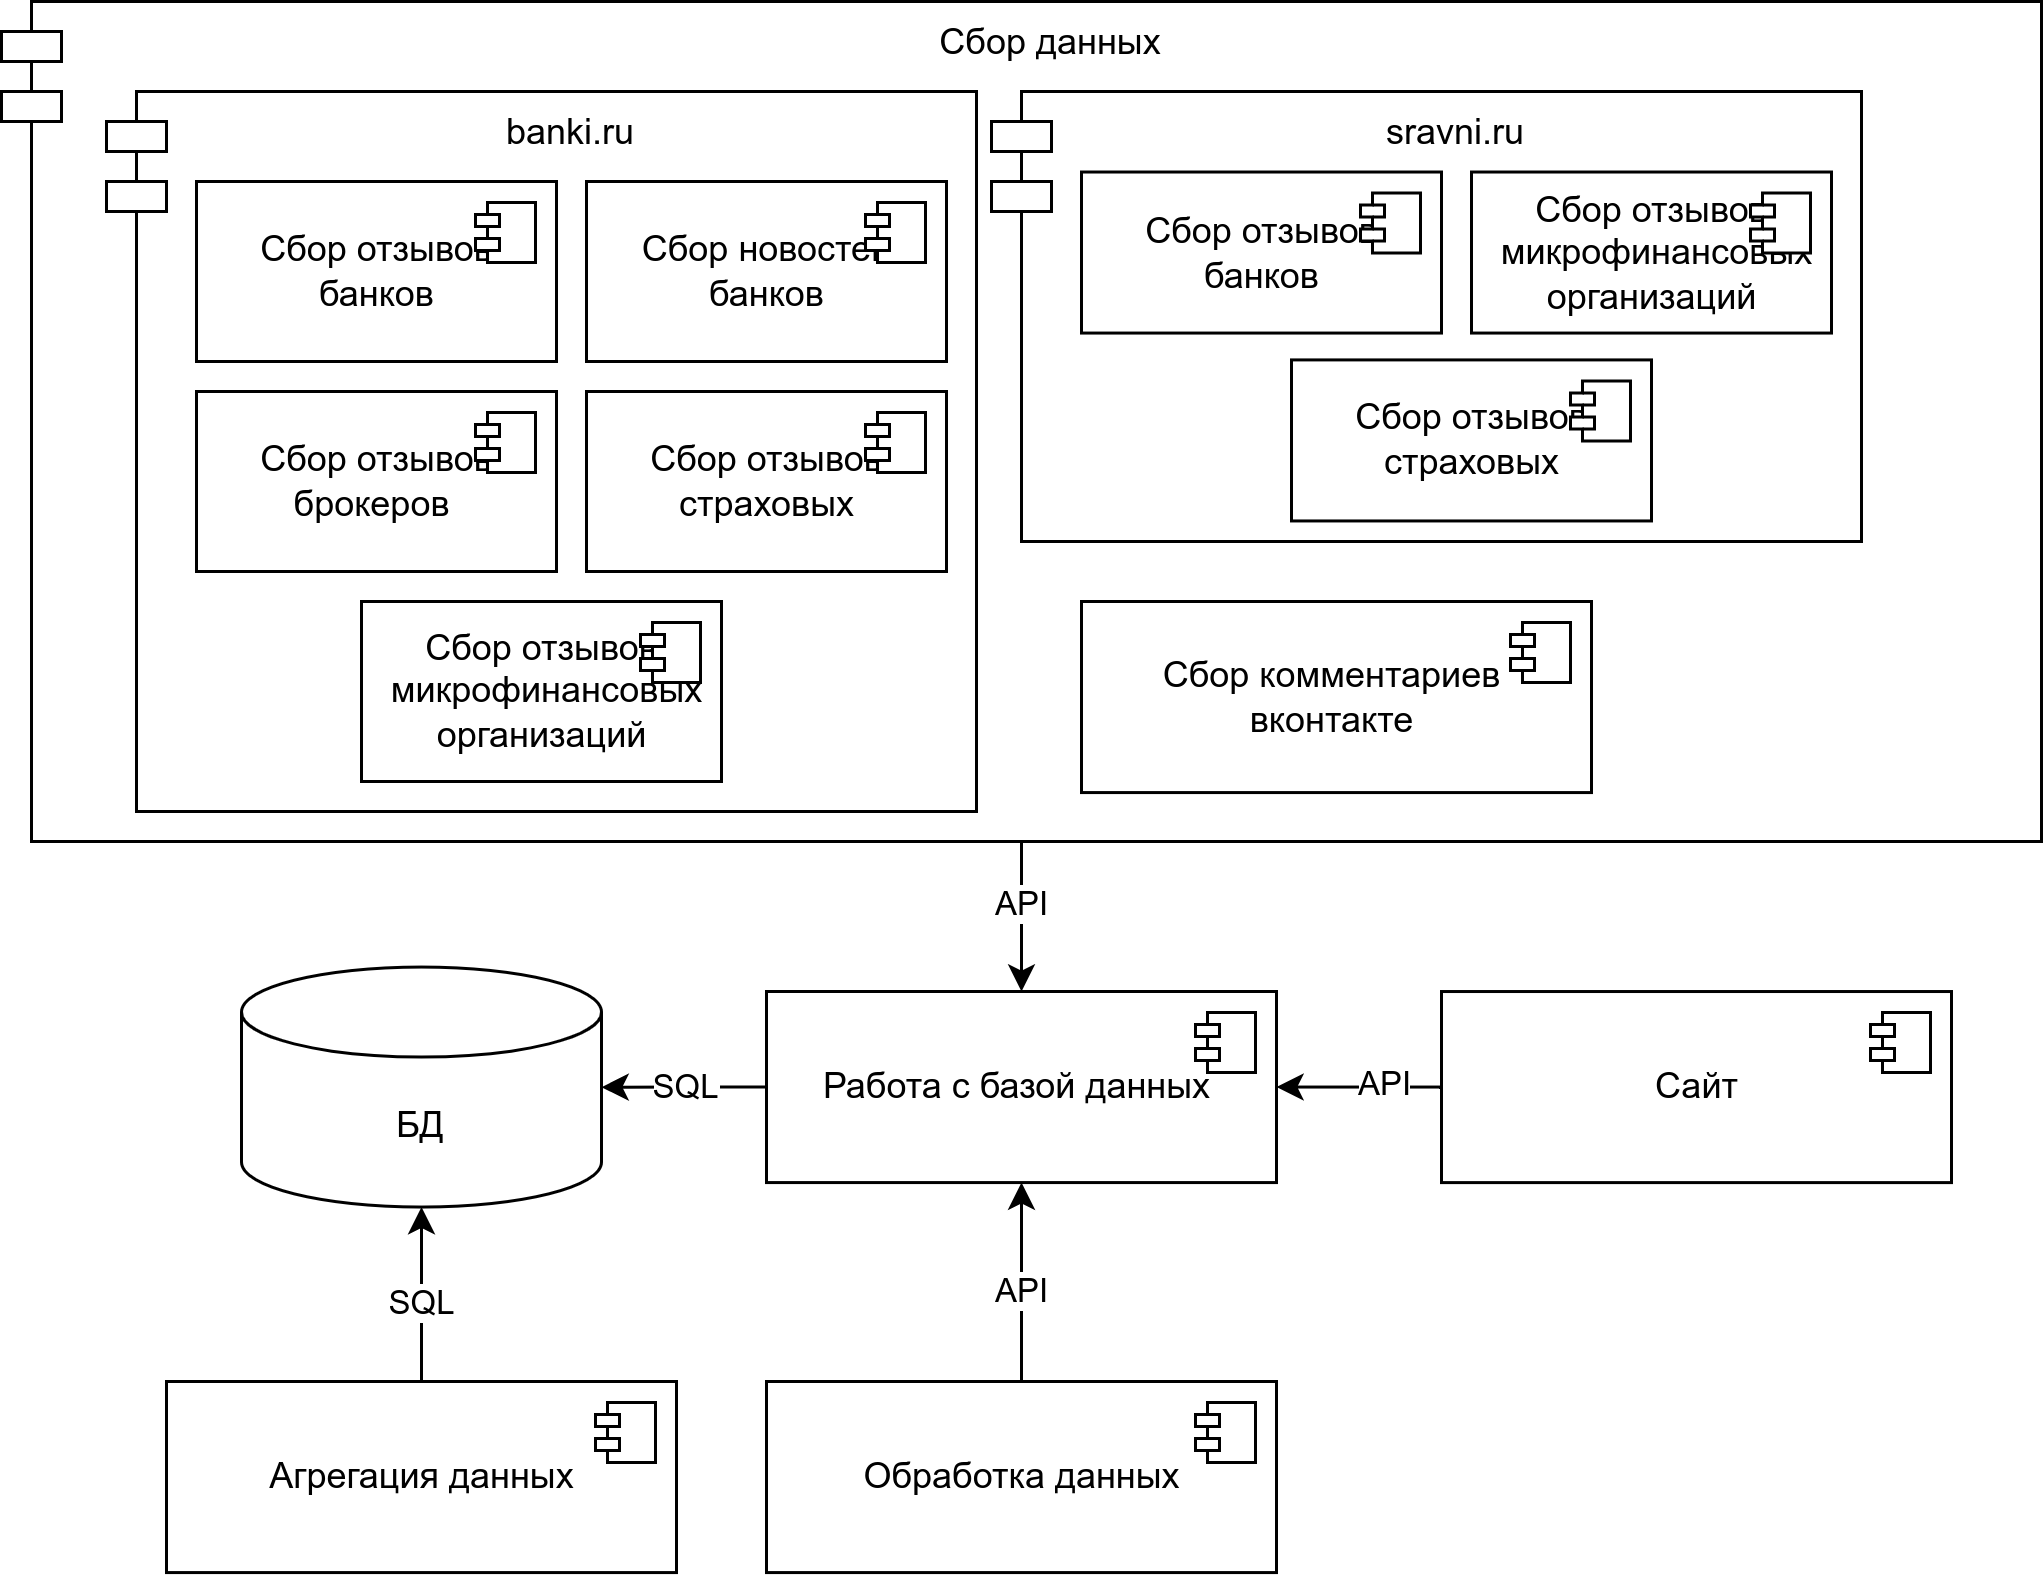
\includegraphics[width=0.8\textwidth]{img/architecture.png}
\caption{\label{fig:architecture}Диаграмма архитектуры системы}
\end{figure}

Сервис для работы с базой данных, который будет обеспечивать сохранение и получение информации из различных сервисов сбора и обработки данных. Для этого будет предоставлен API, который будет использоваться для отправки и получения данных.

Сервисы сбора данных будут отправлять собранные тексты в формате JSON на сервис работы с базой данных с помощью HTTP запросов. Кроме того, информация, необходимая для сбора данных, будет храниться в базах данных соответствующих сервисов, что соответствует принципам микросервисной архитектуры\autocite{ghofrani_challenges_2018}.

Сервис агрегации данных будет периодически обновлять базу данных один раз в день для обеспечения актуальности данных.

Сервис сбора данных будет включать модель машинного обучения, которая будет использоваться для анализа данных, полученных из сервиса сбора данных. После обработки данных, результаты будут отправляться обратно в сервис сбора данных.
\section{Проектирование базы данных}
\label{sec:orgf1a316a}
Исходя из поставленных требований было решено разделить базу данных на 2 подчасти:
\begin{enumerate}
\item Основная база данных будет хранить данные.
\item База данных для агрегации будет позволять быстро получать агрегированные данные.
\end{enumerate}

\subsection{Проектирование основной базы данных}
\label{sec:org0ebd60a}
На основании требований была разработана следующая схема базы данных:

Таблица сфер компаний позволяет в дальнейшей удобно фильтровать данные в зависимости от типа компании.

\begin{center}
\begin{longtblr}[caption={Таблица сфера компании\label{tbl:company_type}}]{colspec={|X[2,l]|X[1,l]|X[3,l]|},rowhead = 1,hlines}
\textbf{Название} & \textbf{Тип} & \textbf{Описание}\\[0pt]
Идентификатор & Целое & Уникальный идентификатор\\[0pt]
Сфера компании & Строка & \\[0pt]
\end{longtblr}
\end{center}

Таблица со списком компании будет хранить основную информации о компаниях.

\begin{center}
\begin{longtblr}[caption={Таблица компаний\label{tbl:companies}}]{colspec={|X[l]|X[l]|X[l]|},rowhead = 1,hlines}
\textbf{Название} & \textbf{Тип} & \textbf{Описание}\\[0pt]
Идентификатор & Целое & Уникальный идентификатор\\[0pt]
Название компании & Строка & \\[0pt]
Описание компании & Строка & Дополнительное поле для сохранения вспомогательной информации о компании\\[0pt]
Лицензия компании & Строка & По лицензии компаний может будет сопоставлять компании на разных сайтах\\[0pt]
Код сферы компании & Целое & Внешний ключ из таблицы Сфера компании\\[0pt]
\end{longtblr}
\end{center}

Аналогично для сфер компаний таблица для типов источников позволяет удобно работать с данными в дальнейшем.

\begin{center}
\begin{longtblr}[caption={Таблица тип источников\label{tbl:source_type}}]{colspec={|X[l]|X[l]|X[l]|},rowhead = 1,hlines}
\textbf{Название} & \textbf{Тип} & \textbf{Описание}\\[0pt]
Идентификатор & Целое & Уникальный идентификатор\\[0pt]
Название типа источника & Строка & \\[0pt]
\end{longtblr}
\end{center}

Таблица источников будет хранить информацию об источниках и когда было последнее обновление данных для них (в полях {}<<состояние сборщика данных>>{} и {}<<дата последнего сбора данных>>{}). Поле {}<<состояние сборщика данных>>{} будет иметь формат json, так как для разных источников информации потребуется сохранять информацию в различном виде и сложно определить наиболее подходящий формат заранее.

\begin{center}
\begin{longtblr}[caption={Таблица источники\label{tbl:sources}}]{colspec={|X[l]|X[l]|X[l]|},rowhead = 1,hlines}
\textbf{Название} & \textbf{Тип} & \textbf{Описание}\\[0pt]
Идентификатор & Целое & Уникальный идентификатор\\[0pt]
Сайт & Строка & Сайт источника\\[0pt]
Код типа источника & Целое & Внешний ключ из таблицы тип источника\\[0pt]
Состояние сборщика данных & JSON & Данные о текущем состояние сборщика данных, если возникнет сбой\\[0pt]
Дата последнего сбора & DateTime & Точка когда сбор данных закончился, для дальнейшего сбора данных\\[0pt]
\end{longtblr}
\end{center}

Аналогично для сфер компаний таблица для типов модели позволяет удобно работать с данными в дальнейшем.

\begin{center}
\begin{longtblr}[caption={Таблица тип модели\label{tbl:model_type}}]{colspec={|X[l]|X[l]|X[l]|},rowhead = 1,hlines}
\textbf{Название} & \textbf{Тип} & \textbf{Описание}\\[0pt]
Идентификатор & Целое & Уникальный идентификатор\\[0pt]
Название модели & Строка & \\[0pt]
\end{longtblr}
\end{center}

Таблица модели позволяет сохранять информацию о различных моделях в дальнейшем.

\begin{center}
\begin{longtblr}[caption={Таблица модели\label{tbl:model}}]{colspec={|X[l]|X[l]|X[l]|},rowhead = 1,hlines}
\textbf{Название} & \textbf{Тип} & \textbf{Описание}\\[0pt]
Идентификатор & Целое & Уникальный идентификатор\\[0pt]
Название модели & Строка & \\[0pt]
Код типа модели & Целое & Внешний ключ на таблицу тип модели\\[0pt]
\end{longtblr}
\end{center}

Таблица текст сохраняет мета информацию о тексте отзыва.

\begin{center}
\begin{longtblr}[caption={Таблицы текст\label{tbl:text}}]{colspec={|X[l]|X[l]|X[l]|},rowhead = 1,hlines}
\textbf{Название} & \textbf{Тип} & \textbf{Описание}\\[0pt]
Идентификатор & Целое & Уникальный идентификатор\\[0pt]
Ссылка & Строка & Ссылка на текст\\[0pt]
Код источника & Целое & Внешний ключ из таблицы источники\\[0pt]
Дата текста & DateTime & Время публикации текста\\[0pt]
Заголовок & Строка & Заголовок текста\\[0pt]
Код компании & Целое & Внешний ключ на компанию\\[0pt]
Количество комментариев & Целое & \\[0pt]
\end{longtblr}
\end{center}

Так как Bert на вход принимает отдельные предложения, было решено сделать для них отдельную таблицу.

\begin{center}
\begin{longtblr}[caption={Таблица предложений\label{tbl:sentence}}]{colspec={|X[l]|X[l]|X[l]|},rowhead = 1,hlines}
\textbf{Название} & \textbf{Тип} & \textbf{Описание}\\[0pt]
Идентификатор & Целое & Уникальный идентификатор\\[0pt]
Код текста & Целое & Внешний ключ из таблицы тексты\\[0pt]
Предложение & Строка & \\[0pt]
Номер предложения & Целое & Порядковый номер предложения в тексте\\[0pt]
\end{longtblr}
\end{center}

Так как результат работы модели может отличать в зависимости от ее типа, то поле {}<<результат>>{} будет массивом.

\begin{center}
\begin{longtblr}[caption={Таблица результатов анализа текстов\label{tbl:text_result}}]{colspec={|X[l]|X[l]|X[l]|},rowhead = 1,hlines}
\textbf{Название} & \textbf{Тип} & \textbf{Назначение}\\[0pt]
Идентификатор & Целое & Уникальный идентификатор\\[0pt]
Код предложения & Целое & Внешний ключ из таблицы предложения\\[0pt]
Код модели & Целое & Внешний ключ из таблицы модели\\[0pt]
Результат & Вещественный массив & Результат работы модели\\[0pt]
Обработано & Логическое & Показатель, обработано ли предложение или нет\\[0pt]
\end{longtblr}
\end{center}

Диаграмма полученной схемы базы данных рис.~\ref{fig:database}.
\subsection{Проектирование базы данных для агрегации}
\label{sec:org430bb3e}
При сборе функциональных требований было выявлено, что надо быстро показывать количество собранных отзывов и индекс компаний.

Обработанные данные из таблицы~\ref{tbl:text_result} агрегируются для каждого квартала и рассчитываются по формуле \ref{eq:ethics}.
\begin{center}
\begin{longtblr}[caption={Таблица для расчета и показа индекса\label{tbl:index_calc}}]{colspec={|X[2,l]|X[1,l]|X[3,l]|},rowhead = 1,hlines}
\textbf{Название} & \textbf{Тип} & \textbf{Описание}\\[0pt]
Идентификатор & Целое & Уникальный идентификатор\\[0pt]
Год & Целое & Год за который был агрегирован индекс\\[0pt]
Квартал & Целое & Квартал за который был агрегирован индекс\\[0pt]
Название модели & Строка & \\[0pt]
Сайт источника & Строка & \\[0pt]
Тип источника & Строка & \\[0pt]
Название компании & Строка & \\[0pt]
Код компании & Целое & Для запросов через API\\[0pt]
Нейтральный & Целое & Количество нейтральных предложений за период\\[0pt]
Позитивный & Целое & Количество позитивных предложений за период\\[0pt]
Негативный & Целое & Количество негативных предложений за период\\[0pt]
Базовый индекс & Вещественное & Индекс для расчета итогового индекса\\[0pt]
Средний индекс & Вещественное & Индекс для расчета итогового индекса\\[0pt]
Std индекс & Вещественное & Индекс для расчета итогового индекса\\[0pt]
Индекс & Вещественное & Рассчитанный индекс\\[0pt]
\end{longtblr}
\end{center}

Собранные отзывы из таблицы~\ref{tbl:text} агрегируются для каждого месяца и рассчитывается количество собранных отзывов за месяц.
\begin{center}
\begin{longtblr}[caption={Таблица для расчета и показа индекса\label{tbl:index_calc}}]{colspec={|X[2,l]|X[1,l]|X[3,l]|},rowhead = 1,hlines}
\textbf{Название} & \textbf{Тип} & \textbf{Описание}\\[0pt]
Идентификатор & Целое & Уникальный идентификатор\\[0pt]
Дата & DateTime & \\[0pt]
Квартал & Целое & Квартал за который был агрегирован индекс\\[0pt]
Тип источника & Строка & \\[0pt]
Сайт & Строка & \\[0pt]
Количество отзывов & Целое & \\[0pt]
\end{longtblr}
\end{center}

Диаграмма полученной схемы базы данных рис.~\ref{fig:database_views}.
\section{Проектирование модуля работы с данными}
\label{sec:org572f928}
Модуль будет представлять собой HTTP API для работой с базой данных.

Для работы с базой данных будут созданы классы, которые представляют ORM-модель для работы с базой данных.

При первом старте приложение будет получаться список компаний (банки, брокеры, микрокредитные организации и страховые) с сайта {}<<Центрального банка России>>{} и помещаться в базу данных. Из этих данных будет собираться лицензия компании и название компании, для микрокредитных организаций дополнительно будет собираться основной государственный регистрационный номер (ОГРН), так как под одной лицензией может работать несколько компаний. При последующих стартах приложение будет проверяться, что в каждом списке есть компании и новые компании не будут выгружаться.

Далее создаются объекты класса Bank с использованием полученных данных и добавляются в список  cbr\_banks, затем он возвращается как результат работы функции.

Таким образом, принцип работы данного алгоритма заключается в извлечении необходимых данных из HTML-кода веб-страницы и преобразовании их в объекты класса Bank, что позволяет автоматизировать процесс получения и анализа информации о компаниях. Диаграмма классов рис.~\ref{fig:cbr_parser_class}.

\begin{center}
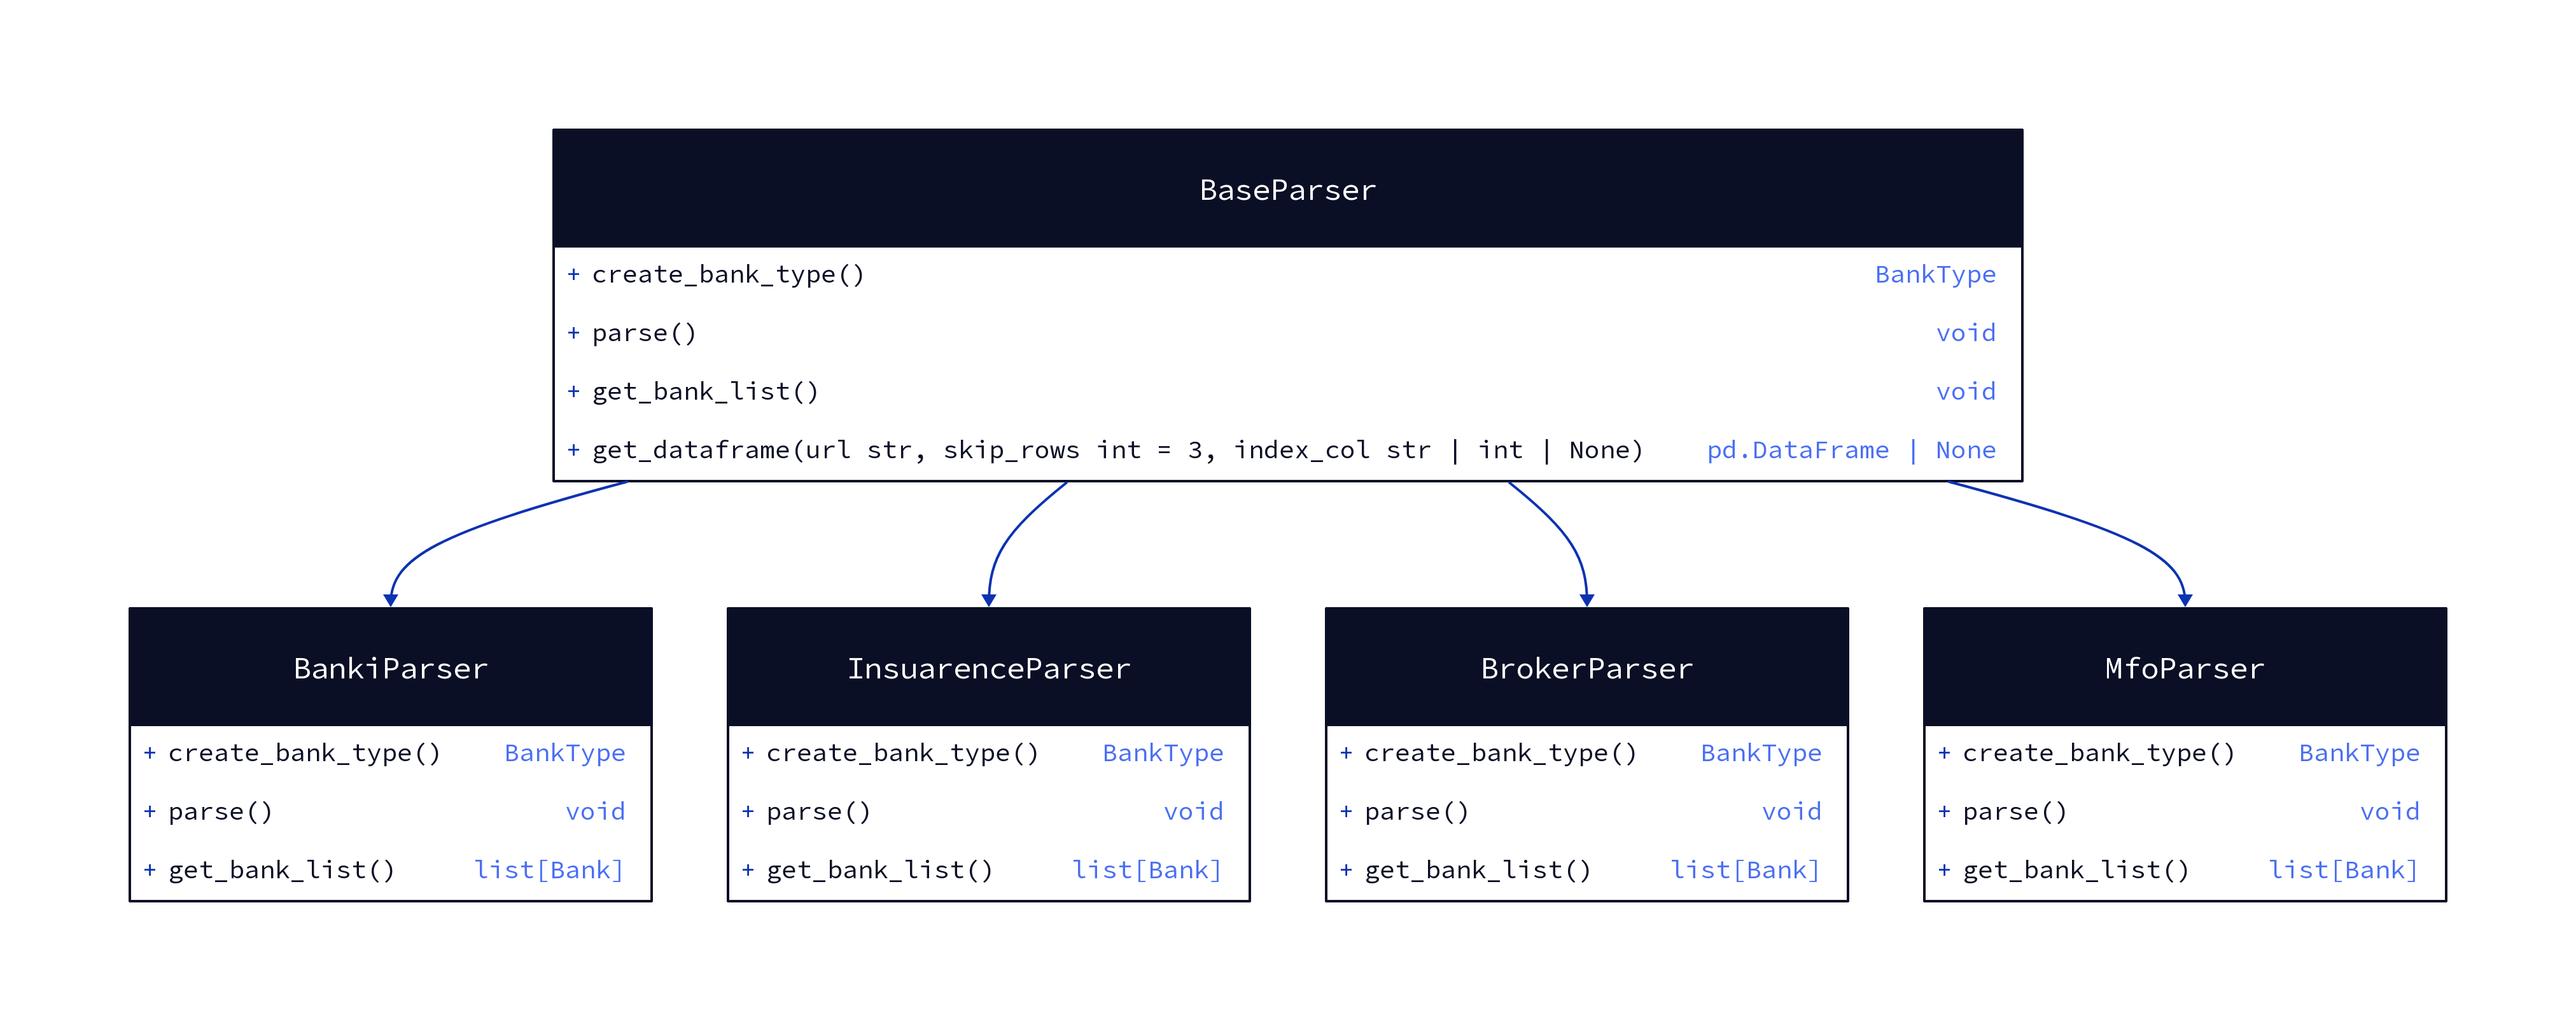
\includegraphics[width=.9\linewidth]{img/d2/cbr_parser_class.png}
\end{center}

Для работы с источниками текстов необходимо сделать запросы для типов источников и самих источников. Также для обновления состояния сборщика данных надо сделать отдельный метод \texttt{PATCH}, который позволит обновлять время и состояние источника данных по идентификатору. Также при создании источника будет проверяться существует ли такой тип источника или нет. Если его не существует, то такой тип будет создаваться.

Сохранение текстов будет доступно по методу \texttt{POST} c передачей данных о тексте и состоянии сборщика данных. При выполнении запроса должно обновляться состояние сборщика данных, а каждый текст должен сохраняться, как набор предложений. При получении предложений должны выбираться такие предложения, которые еще не обработаны моделью.

Работа с моделями будет происходить аналогично источникам. При сохранении модели будет проверяться есть ли такой тип модели или нет. Если его нет, то он будет создан.

Также необходима возможность получения списка компаний с помощью API по различным сферам работы.

В результате проектирования должно получиться API, которое реализует запросы представленные в таблице ~\ref{tbl:api_doc}.
\section{Проектирование модуля агрегации данных}
\label{sec:org7c8efc5}
Для построения индекса этичности компаний будет ежедневно агрегироваться база данных и перестраиваться индексы.
\section{Проектирование модуля сбора данных}
\label{sec:orgfe70059}
У всех сборщиков данных одинаковый принцип работы (рис.~\ref{fig:parser_flow}):
\begin{enumerate}
\item Сборщик данных запрашивает у модуля работы с базой данных список сохраненных компаний. Модуль отвечает на запрос, отправляя список сохраненных компаний обратно.
\item Сборщик данных запрашивает у сайта для сбора данных список компаний на сайте. Сайт отправляет список компаний обратно в сборщик данных.
\item После получения списка компаний, сборщик данных сохраняет только те компании, которые уже есть в основной базе данных. Это делается для того, чтобы связать компании которые представлены на сайте и в базе данных.
\item Затем, сборщик данных начинает собирать данные для каждой компании из списка. Это может быть сделано путем отправки запросов к API сайта или сканирования страниц сайта для поиска нужных данных. Собранные данные затем сохраняются в основной базе данных. Сбор данных будет происходить до тех пор пока не соберутся все отзывы для компании, или дата отзыва дойдет до даты предыдущего сбора данных.
\end{enumerate}

Для реализации сборщиков данных было решено сделать базовый класс, который представляет собой интерфейс с функцией \texttt{parse}. Из него наследуются интерфейсы для сбора данных для каждого сайта (banki.ru, sravni.ru, vk.com). Диаграмма классов рис.~\ref{fig:parser_class_diagram}. От этих базовых классов для каждого сайта будут наследоваться классы, которые собирают отзывы компаний из различных сфер. Было выбрано такое решение, так как представление информации в рамках одного сайта в различных разделах может сильно различаться. Также у каждого сборщика данных будет своя база данных для сохранения информации о компаниях.

\subsection{Проектирование сбора данных с banki.ru}
\label{sec:org5036a1a}
Для получения данных с сайта banki.ru будут отправляться запросы на их внутренний API. Для запросов надо иметь идентификатор компании с сайта, также надо иметь идентификатор компании из модуля работы с базой данных. Исходя из требований получилась база данных ~\ref{tbl:banki_ru}. Диаграмма полученной схемы базы данных рис.~\ref{fig:database_banki_ru}.

\begin{center}
\begin{longtblr}[caption={Таблица для сайта banki.ru\label{tbl:banki_ru}}]{colspec={|X[2,l]|X[1,l]|X[3,l]|},rowhead = 1,hlines}
\textbf{Название} & \textbf{Тип} & \textbf{Описание}\\[0pt]
Идентификатор & Целое & Уникальный идентификатор\\[0pt]
Идентификатор компании & Целое & Идентификатор банка в основной базе данных\\[0pt]
Имя компании & Строка & \\[0pt]
Код компании & Строка & Код компании для запросов по API\\[0pt]
\end{longtblr}
\end{center}

С этого сайта будут собираться данные о компаниях из пяти сфер:
\begin{enumerate}
\item \textbf{Отзывы на банки.}
Список банков будет получаться из \url{https://www.banki.ru/widget/ajax/bank\_list.json}. Затем они будут сравниваться по номеру лицензии с банками, которые есть в базе данных. Для получения отзывов о банках будут отправляться запросы на \url{https://www.banki.ru/services/responses/list/ajax/} и в параметры ссылки будет передаваться код банка и номер страницы с отзывами и из полученного json будут собираться данные об отзывах.
\item \textbf{Новости о банках.}
В качестве списка компаний будет использоваться такой же список, как и для банков. Для получения текста новостей сначала будет собираться список новостей для компании. Для этого будут отправляться запросы на \url{https://www.banki.ru/banks/bank/\{bank.bank\_code\}/news/} в зависимости от банка. Затем по каждой ссылке будет обрабатываться html код страницы и собираться текст новости.
\item \textbf{Отзывы на страховые компании.}
Список компаний будет получаться из \url{https://www.banki.ru/insurance/companies/}. Затем они будут сравниваться по номеру лицензии со страховыми, которые есть в базе данных. После этого будут собираться отзывы по \url{https://www.banki.ru/insurance/companies/}. Затем из каждой страницы компании для будет обрабатываться html код страницы и браться данные отзывов.
\item \textbf{Отзывы на брокеров.}
Для получения списка компаний данные будут браться из \url{https://www.banki.ru/investment/brokers/list/}. Затем они будут сравниваться по номеру лицензии с брокерами, которые есть в базе данных. После этого будут собираться отзывы по \url{https://www.banki.ru/investment/responses/company/broker/}. Затем из каждой страницы компании для будет обрабатываться html код страницы и браться данные отзывов.
\item \textbf{Отзывы на микрокредитные организации.}
Для получения списка компаний данные будут браться из \url{https://www.banki.ru/microloans/ajax/search}. Затем они будут сравниваться по номеру лицензии и ОГРН с компания, которые есть в базе данных. После этого будут собираться отзывы по \url{https://www.banki.ru/microloans/responses/ajax/responses/}. Затем из полученного json собираются отзывы о компании.
\end{enumerate}
В конце сбора данных для каждого типа компаний собранные отзывы будут отправляться в модуль работы с базой данных.
\subsection{Проектирование сбора данных с sravni.ru}
\label{sec:orgfa69610}
Для получения данных с сайта sravni.ru будут отправляться запросы на их внутренний API. Для запросов надо иметь идентификатор компании с сайта, также надо иметь идентификатор компании из модуля работы с базой данных, также для некоторых запросов надо иметь псевдоним компании (alias). Исходя из требований получилась база данных~\ref{tbl:sravni_ru}. Диаграмма полученной схемы базы данных рис.~\ref{fig:database_sravni_ru}.

\begin{center}
\begin{longtblr}[caption={Таблица для сайта sravni.ru\label{tbl:sravni_ru}}]{colspec={|X[2,l]|X[1,l]|X[3,l]|},rowhead = 1,hlines}
\textbf{Название} & \textbf{Тип} & \textbf{Описание}\\[0pt]
Идентификатор & Целое & Уникальный идентификатор\\[0pt]
Идентификатор компании & Целое & Идентификатор компании в основной базе данных\\[0pt]
Код банка в sravni.ru & Целое & \\[0pt]
Старый код компании в sravni.ru & Целое & \\[0pt]
Псевдоним компании & Строка & \\[0pt]
Название компании & Строка & \\[0pt]
\end{longtblr}
\end{center}
Диаграмма полученной схемы базы данных рис.~\ref{fig:database_sravni_ru}

С этого сайта будут собираться данные о компаниях из трех сфер:
\begin{enumerate}
\item \textbf{Отзывы на банки.}
Список банков будет получаться из \url{https://www.sravni.ru/proxy-organizations/organizations} с параметром \texttt{organizationType} равным \texttt{bank}. Затем они будут сравниваться по номеру лицензии с банками, которые есть в базе данных. Для получения отзывов о банках будут отправляться запросы на \url{https://www.sravni.ru/bank/\{bank\_info.alias\}/otzyvy/} и в параметры ссылки будет передаваться псевдоним банка и номер страницы с отзывами. И из полученного json будут собираться данные об отзывах.
\item \textbf{Отзывы на страховые компании.}
Список банков будет получаться из \url{https://www.sravni.ru/proxy-organizations/organizations} с параметром \texttt{organizationType} равным \texttt{insuranceCompany}. Затем они будут сравниваться по номеру лицензии со страховыми, которые есть в базе данных. Для получения отзывов о банках будут отправляться запросы на \url{https://www.sravni.ru/strakhovaja-kompanija/\{bank\_info.alias\}/otzyvy/} и в параметры ссылки будет передаваться псевдоним страховой и номер страницы с отзывами. И из полученного json будут собираться данные об отзывах.
\item \textbf{Отзывы на микрокредитные организации.}
Список банков будет получаться из \url{https://www.sravni.ru/proxy-organizations/organizations} с параметром \texttt{organizationType} равным \texttt{mfo}. Затем они будут сравниваться по номеру лицензии и ОГРН с компаниями, которые есть в базе данных. Для получения отзывов о банках будут отправляться запросы на \url{https://www.sravni.ru/zaimy/\{bank\_info.alias\}/otzyvy/} и в параметры ссылки будет передаваться псевдоним банка и номер страницы с отзывами. И из полученного json будут собираться данные об отзывах.
\end{enumerate}
В конце сбора данных для каждого типа компаний собранные отзывы будут отправляться в модуль работы с базой данных.
\subsection{Проектирование сбора данных с vk.com}
\label{sec:org85698ca}
Для получения на сайт vk.com будут отправляться запросы на их API. Для этого предварительно будут собраны данные о всех организациях, которые у них представлены на сайте и перемещены в базу данных \ref{tbl:vk_com}. Диаграмма полученной схемы базы данных рис.~\ref{fig:database_vk_com}.
\begin{center}
\begin{longtblr}[caption={Таблица для сайта vk.com\label{tbl:vk_com}}]{colspec={|X[2,l]|X[1,l]|X[3,l]|},rowhead = 1,hlines}
\textbf{Название} & \textbf{Тип} & \textbf{Описание}\\[0pt]
Идентификатор & Целое & Уникальный идентификатор\\[0pt]
Идентификатор на vk.com & Строка & \\[0pt]
Имя компании & Строка & \\[0pt]
Домен компании на vk.com & Строка & \\[0pt]
\end{longtblr}
\end{center}

Для доступа к API будет зарегистрировано приложение для получения ключа к нему. Для каждой компании будут выгружаться посты пока дата последней выгрузки не более чем дата последнего поста для этого будет отправляться запрос на \url{https://api.vk.com/method/wall.get}, куда будет подставляться токен приложения и идентификатор группы. Затем для каждого поста будут выгружаться комментарии по методу \url{https://api.vk.com/method/wall.getComments}, а затем отправляться в модуль работы с базой данных.
\section{Проектирование модуля обработки данных}
\label{sec:orgb5ab904}
Данный модуль будет обрабатывать полученные отзывы с помощью полученной модели. Для этого каждый день он будет запускаться, получать тексты из модуля работы с базой данных и отправлять из обратно.
\section{Выводы по главе}
\label{sec:org74760c0}
В данной главе были представлены результаты проектирования системы и ее отдельных модулей и их взаимодействие, включая базы данных и API, согласно выявленным требованиям из первой главы. Каждый модуль был спроектирован с учетом принципов микросервисной архитектуры и обеспечивает функциональность, необходимую для реализации системы в целом.

Была спроектирована база данных для хранения информации об отзывах, источниках, моделях и компаниях. Она была спроектированы с учетом требований к масштабируемости и производительности системы.

Было проведено проектирование методов для лучшего подбора метода обработки текста и модели классификации. Для этого была подобрана метрика, которая позволит лучшим образом отразить результат подбора моделей.

Эти результаты будут использоваться при разработке и реализации системы в следующих этапах проекта.
\chapter{Реализация системы}
\label{sec:orgc0b8fc6}
В данной главе описывается реализация системы и каждого модуля, обучение модели.

Этап реализации можно разделить на пункты:
\begin{enumerate}
\item Реализация базы данных.
\item Реализации модулей для собора, работы и агрегации данных.
\item Обучение модели и реализация модуля обработки данных.
\item Развертывание системы.
\end{enumerate}
\section{Реализация определения наиболее подходящей модели}
\label{sec:orgf3e0b64}
\subsection{Обучение алгоритмов обработки естественного языка}
\label{sec:org3ec88e2}
Перед обучением алгоритмов надо обработать текст, чтобы повысить их эффективность. В первую очередь была осуществлена очистка от распространенных слов, также известных как стоп-слова, и были удалены знаки пунктуации.

Для лемматизации слов была применена библиотека spaCy\autocite{boyd_explosion_2023}, которая предоставила доступ к модели для русского языка {}<<ru\_core\_news\_md>>{}. Лемматизация является важным этапом, поскольку она помогает уменьшить размерность векторного пространства, используемого в методах анализа текстов, таких как мешок слов и TF-IDF.

Затем был произведен подсчет количество вхождений каждого слова \ref{fig:word_freq_total}. Дополнительно, из текстов были удалены слова, которые встретились менее 10 раз, так как они вносят излишнюю сложность в векторное пространство. В общей сложности такие слова составляют 85\% от общего числа слов \ref{fig:word_freq_low}.

\begin{figure}[h!]
\centering
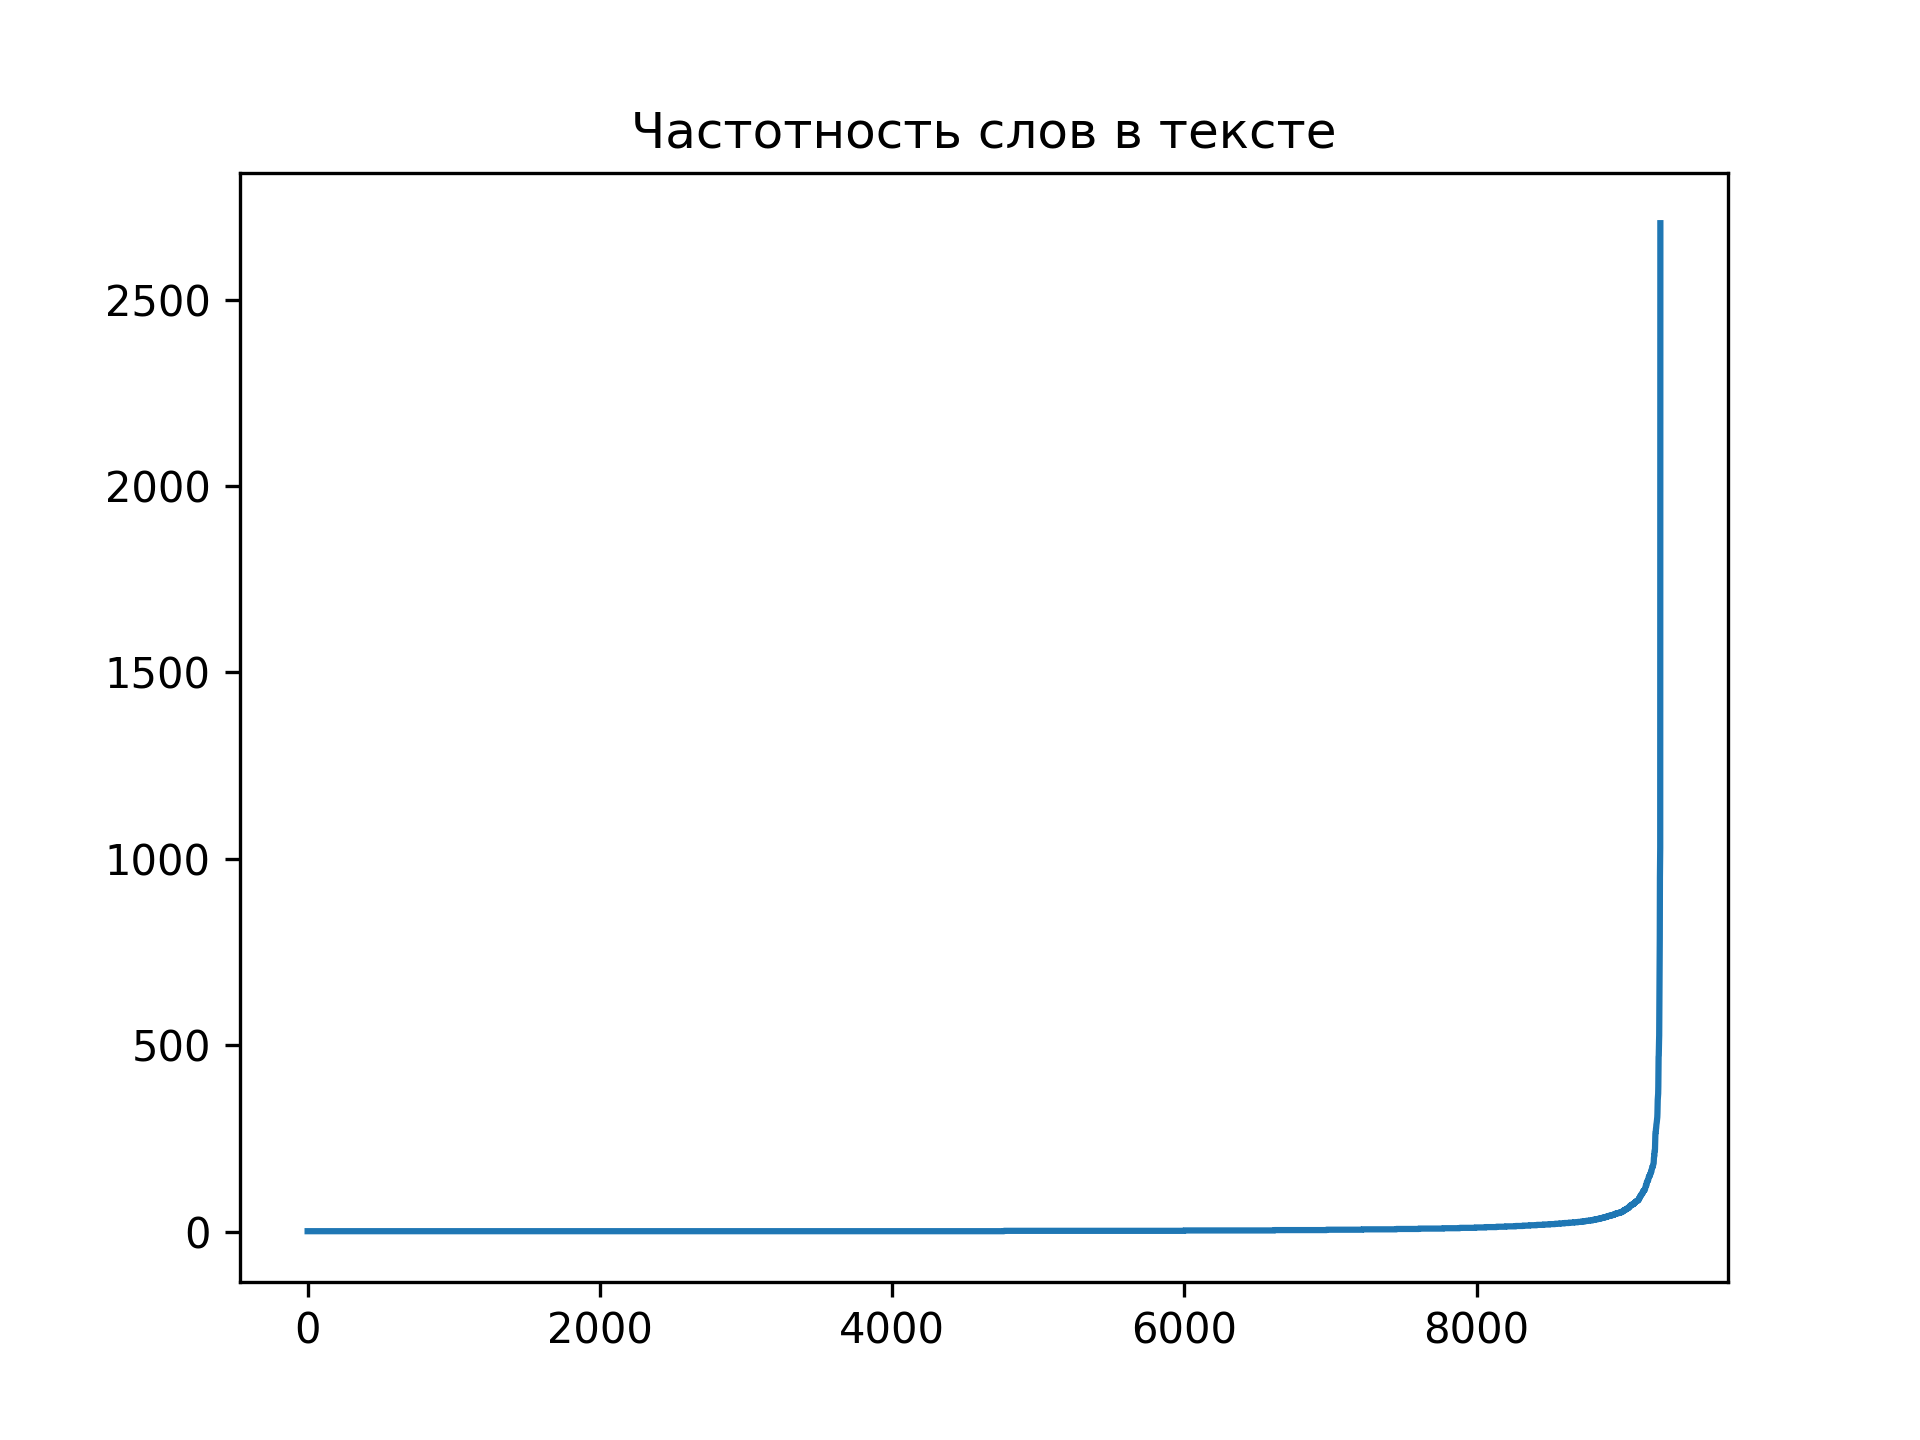
\includegraphics[width=0.8\textwidth]{img/word_freq_total.png}
\caption{\label{fig:word_freq_total}График распространенности слов}
\end{figure}

\begin{figure}[h]
\centering
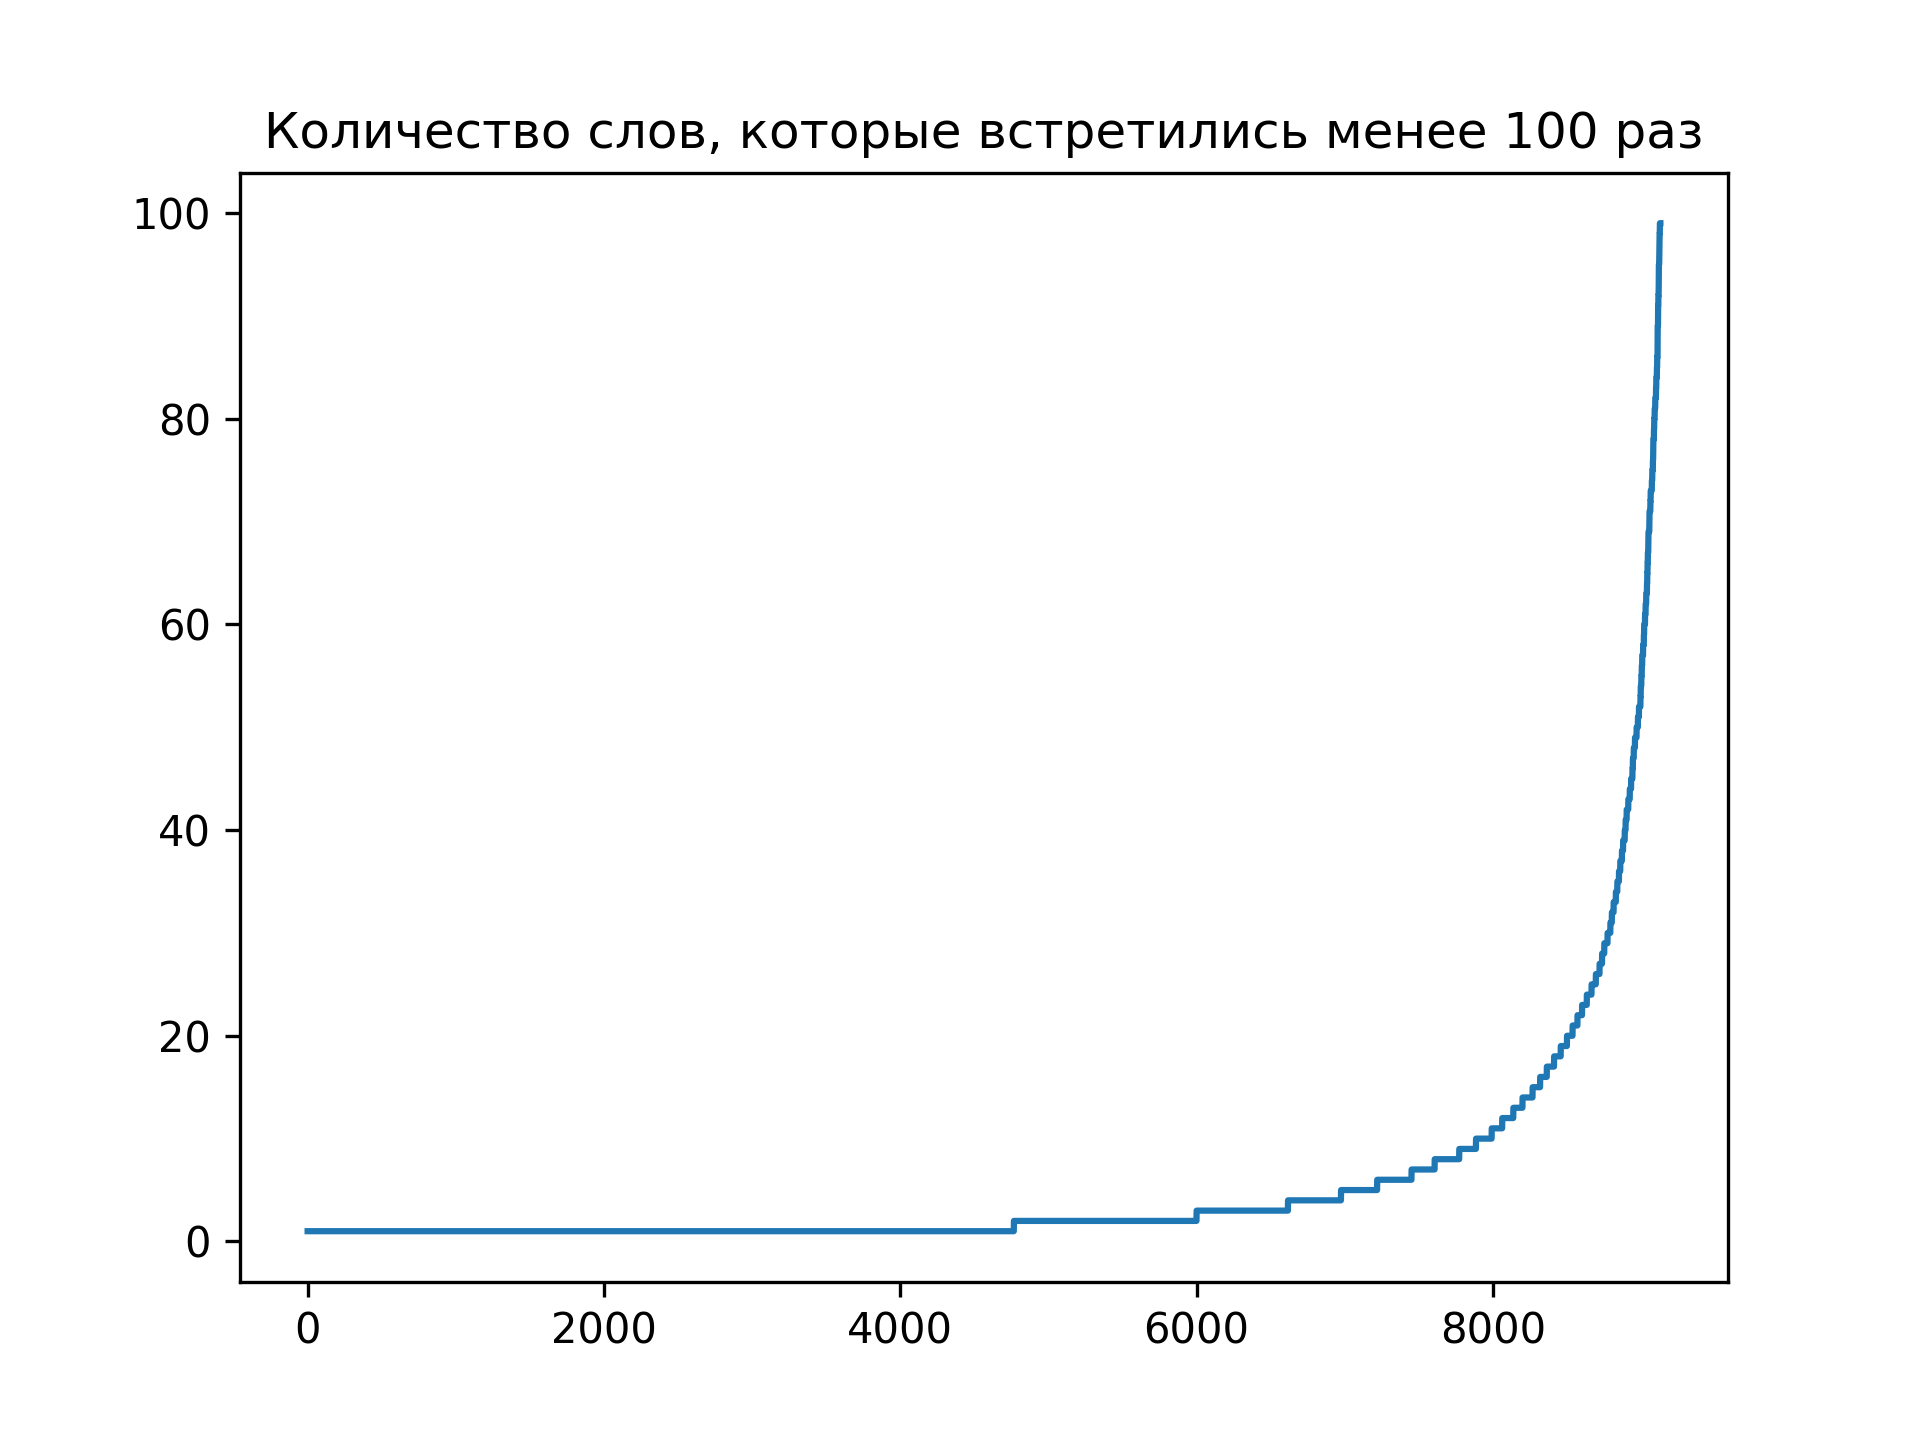
\includegraphics[width=0.8\textwidth]{img/word_freq_low.png}
\caption{\label{fig:word_freq_low}График распространенности слов, которые встретились меньше 100 раз}
\end{figure}

В результате работы алгоритма из текста {}<<Тем самым оставив меня без средств к существованию, тем более я многодетный отец, единственный кормилец семьи!!!>>{} получится {}<<самым оставить средство единственный семья>>{}. Такие тексты подавались на вход мешка слов, TF-IDF и FastText.

Для обработки текста с использованием модели Word2Vec была выбрана модель {}<<word2vec-ruscorpora-300>>{} \autocite{kutuzov_webvectors_2017} из библиотеки gensim\autocite{rehurek_software_2010}. Однако, для корректной работы этой модели, необходимо добавить часть речи к каждому слову. Например, для слова {}<<человек>>{} необходимо добавить метку {}<<NOUN>>{}, так как оно является существительным. Таким образом, входными данными для модели должно быть {}<<человек\textsubscript{NOUN}>>{}. Однако, такое преобразование текста усложняет использование данной модели, так как требуется дополнительная модель для определения частей речи слова. В связи с этим, было принято решение дополнительно воспользоватсья реализацией Word2Vec из библиотеки Navec.

Для обработки текста с помощью BERT будет использоваться 2 модели:
\begin{enumerate}
\item Модель от \texttt{DeepPavlov} \texttt{rubert-base-cased}~\autocite{kuratov_adaptation_2019}, она обучена на русской Википедии и данных из Вконтаке
\item Модель от \texttt{blanchefort} \texttt{rubert-base-cased-sentiment-rurewiews}, за основу этой модели взят \texttt{rubert-base-cased} и был дообучен на данных отзывов, твиттера и данных из медицинский учреждений.
\end{enumerate}

В обе модели будет подаваться как исходный, необработанный текст, так и обработанный текст. Исходный текст используется, поскольку данные модели обучены на большом объеме текста и способны учитывать контекст каждого слова внутри предложения, что делает их более устойчивыми и позволяет достичь более точных результатов.

Кроме того, для оценки качества работы модели будет проведено дообучение модели RuBERT на специально собранных данных. Дообучение будет выполняться путем решения задачи классификации предложений. Для этого будет добавлен слой нейронов к предобученной модели, принимающий векторные представления исходного текста и предсказывающий вероятности принадлежности к различным классам. Этот слой называется {}<<головой классификации>>{} (classification head).

Модель была дообучена в течение 7 эпох на собранных данных, при этом последовательно размораживались слои модели. Для лучшего качества обучения модели использовался оптимизатор \texttt{Adam}~\autocite{kingma_adam_2017}. В результате дообучения были достигнуты следующие значения метрики F1 0.75 при дообучении последнего слоя и 0.77 при дообучении последних двух слоев. Эти результаты свидетельствуют о достигнутом качестве модели в решении задачи классификации текстов.

\begin{figure}[h]
\centering
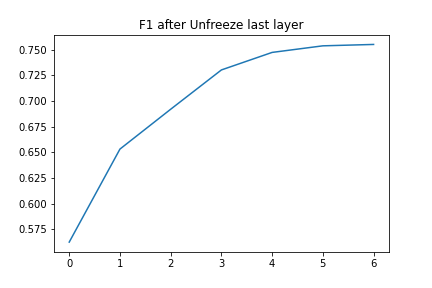
\includegraphics[width=0.8\textwidth]{img/DeepPavlovrubert-base-cased F1 Unfreeze last layer.png}
\caption{\label{fig:bert_unfreeze_last}График изменения метрики F1 при обучении последнего слоя}
\end{figure}

\begin{figure}[h]
\centering
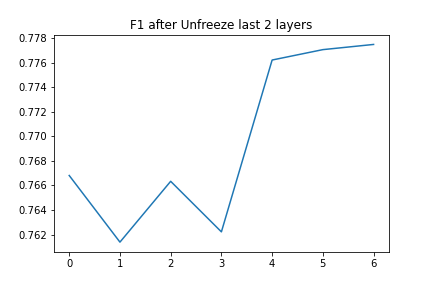
\includegraphics[width=0.8\textwidth]{img/DeepPavlovrubert-base-cased F1 Unfreeze last 2 layers.png}
\caption{\label{fig:bert_unfreeze_two_last}График изменения метрики F1 при обучении последних 2 слоев}
\end{figure}

Для получения эмбеддингов из моделей BERT в цикле в модель подавались предложения и брались данные из последнего слоя и сохранялись.
\subsection{Обучение алгоритмов классификации}
\label{sec:orgc58db8a}
Для лучшего сохранения результатов использовалась библиотека MLFlow\autocite{chen_developments_2020}. Она поможет лучше сохранять и следить за результатами обработки. Пример интерфейса \ref{fig:mlfow_ui}. Для подбора гиперпараметров будет использоваться библиотека Optuna\autocite{akiba_optuna_2019}.

Для удобной интеграции с MLFlow цикл обучения каждой модели помещался в отдельную папку. Тип данных, который принимает на вход модель получается из аргументов с которым она запущена. Затем для каждой модели запускается 30 итераций для подбора гиперпараметров с помощью optuna. Для каждой итерации в MLFlow сохраняется параметры с которыми обучалась модель и результат метрики F1. После обучения всех моделей для подбора гиперпараметров выбираются наиболее оптимальные параметры и обучается итоговая модель и сохраняется в MLFlow. В итоге каждая модель запускалась с каждым типом обработки текста.
\subsection{Результаты}
\label{sec:orga9610fb}
В результате получилось, что лучший результат дало дообучение RuBERT и логистическая регрессия \ref{fig:training_res}.

\begin{figure}[h]
\centering
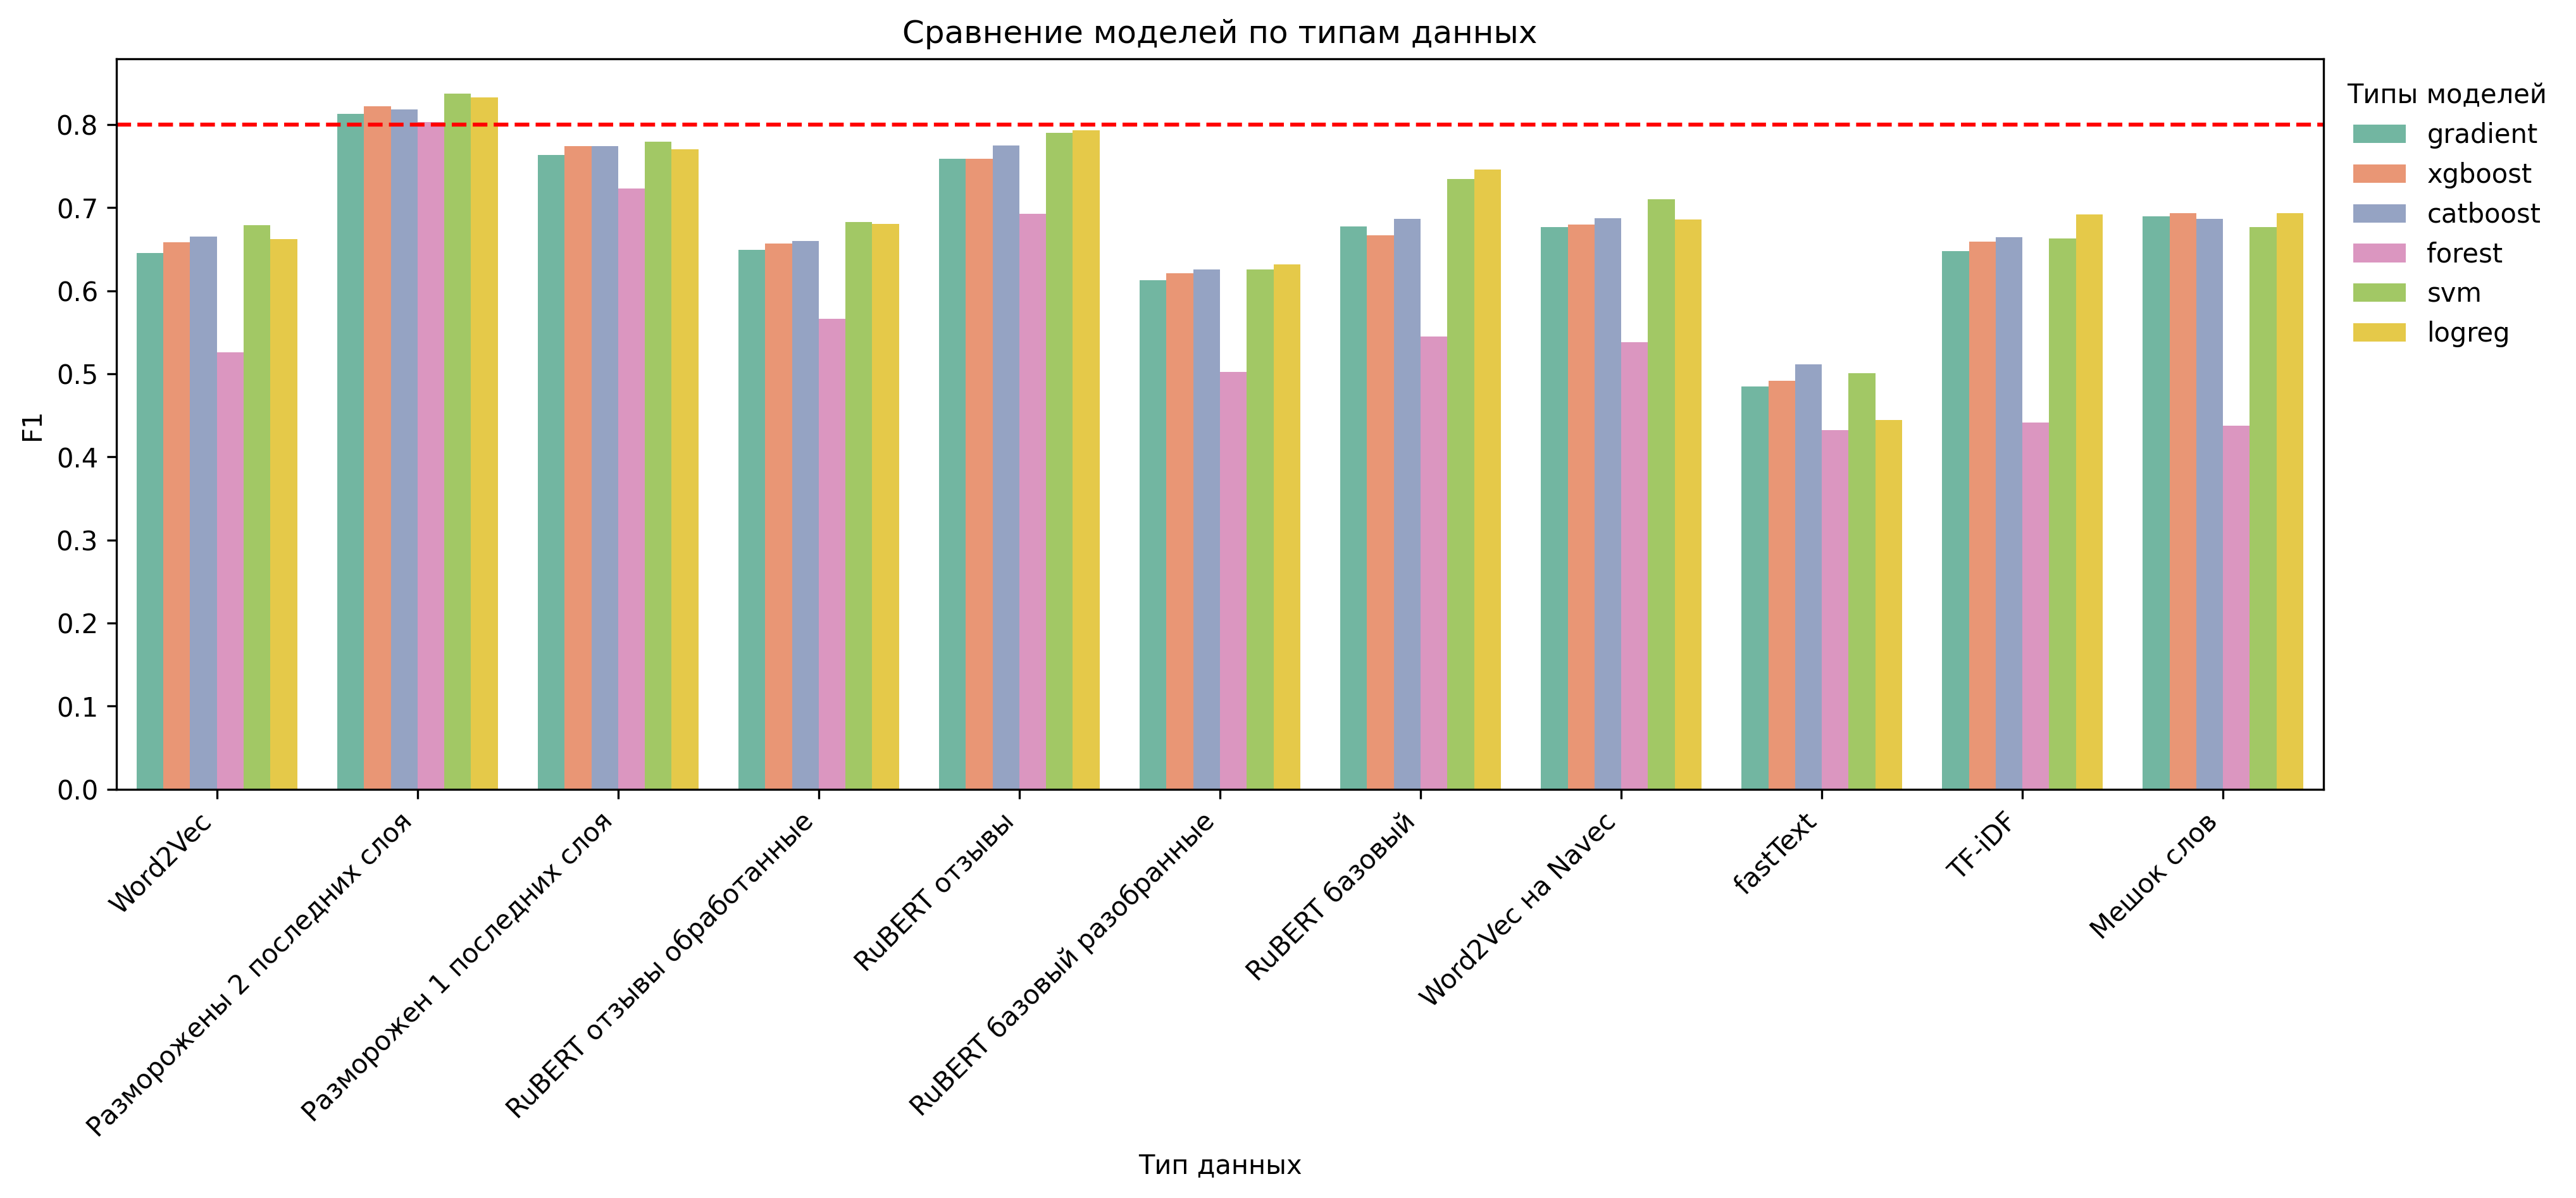
\includegraphics[width=0.8\textwidth]{img/runs.png}
\caption{\label{fig:training_res}Результат обучения моделей}
\end{figure}

\begin{center}
\begin{longtblr}[caption={Таблица результатов обучения моделей\label{tbl:model_data_compare}}]{colspec={|X[2,l]|X[r]|X[r]|X[r]|X[r]|X[r]|X[r]|},rowhead = 1,hlines}
\textbf{Тип входных данных} & \textbf{logreg} & \textbf{svm} & \textbf{forest} & \textbf{gradient} & \textbf{xgboost} & \textbf{catboost}\\[0pt]
Мешок слов & 0.69 & 0.68 & 0.44 & 0.69 & 0.69 & 0.69\\[0pt]
TF-IDF & 0.69 & 0.66 & 0.44 & 0.65 & 0.66 & 0.66\\[0pt]
Word2Vec & 0.66 & 0.68 & 0.53 & 0.65 & 0.66 & 0.67\\[0pt]
Word2Vec Navec & 0.69 & 0.71 & 0.54 & 0.68 & 0.68 & 0.69\\[0pt]
fastText & 0.44 & 0.5 & 0.43 & 0.48 & 0.49 & 0.51\\[0pt]
RuBERT базовый & 0.75 & 0.73 & 0.54 & 0.68 & 0.67 & 0.69\\[0pt]
RuBERT базовый обработанные тексты & 0.63 & 0.63 & 0.5 & 0.61 & 0.62 & 0.63\\[0pt]
RuBERT эмоции & 0.79 & 0.79 & 0.69 & 0.76 & 0.76 & 0.78\\[0pt]
RuBERT эмоции обработанные тексты & 0.68 & 0.68 & 0.57 & 0.65 & 0.66 & 0.66\\[0pt]
RuBERT разморожен 1 последних слоя & 0.77 & 0.78 & 0.72 & 0.76 & 0.77 & 0.77\\[0pt]
RuBERT разморожены 2 последних слоя & 0.83 & 0.83 & 0.8 & 0.81 & 0.82 & 0.82\\[0pt]
\end{longtblr}
\end{center}
\section{Реализация базы данных}
\label{sec:org9ded23e}
Для хранения информации в системе была выбрана СУБД PostgreSQL. Для создания базы данных был выбран подход {}<<code first>>{}, который позволяет определить структуру базы данных в виде классов на языке Python. Для этого использовалась библиотека Sqlalchemy~\autocite{bayermichael_architecture_2012}, которая обеспечивает ORM-модель для работы с базами данных. При запуске приложения база данных будет создаваться автоматически на основе определенных классов.

Для определения структуры базы данных был создан базовый класс \texttt{DeclarativeBase}, который является родительским для всех классов, определяющих таблицы базы данных. Каждая таблица базы данных определяется в виде отдельного класса, который наследует базовый класс и содержит определения столбцов и связей между таблицами.

Для ускорения работы запросов все поля, которые являются внешними ключами были проиндексированы. Также в таблице с информацией о текстах были добавлены индексы, которые извлекают из даты год и квартал.

Для обеспечения возможности модернизации базы данных в дальнейшем была использована библиотека alembic, которая обеспечивает миграции базы данных и позволяет вносить изменения в структуру базы данных без потери данных.
\section{Реализация модуля работы с базой данных}
\label{sec:org2f85cfb}
Для реализации API используется асинхронный фреймворк FastAPI и для взаимодействии с базой данных асинхронная библиотека asyncpg. Для валидации приходящих данных и ответов для каждого запроса была создана своя модель с помощью библиотеки Pydantic. Также с помощью Pydantic был сделан класс для получения строки подключения к базе данных из переменных окружения.

При старте приложения сначала проверятся подключение с базой данных и проверяется ее версия, если она не актуальна, то выполняются миграции для ее актуализации. Затем проверятся список компаний, если список компаний пустой, то собирается данные о банках, брокера, страховых и микрофинансовых организациях.

Информация о банках будет собираться по ссылке \url{https://www.cbr.ru/banking\_sector/credit/FullCoList/}. Алгоритм начинается с получения объекта BeautifulSoup~\autocite{richardsonleonard_beautiful_2007}, который содержит HTML-код веб-страницы. Затем происходит итерация по всем элементам таблицы, начиная со второй строки, так как в первой находится заголовки для каждой колонки. Для каждой строки таблицы находятся все ячейки, извлекаются регистрационный номер (номер лицензии) и название банка. В списке также есть платежные небанковские кредитные организации, которые имеют буквы на конце лицензии, например \texttt{3511-К} у {}<<Деньги.Мэйл.Ру>>{}. Для этого такие номера будут разделяться по {}<<->>{} и браться номер и преобразовываться в число. Затем собранные данные помещаются в базу данных.

Для сбора данных о брокерах будет обрабатываться excel файл, который доступен по ссылке \url{https://www.cbr.ru/vfs/finmarkets/files/supervision/list\_brokers.xlsx}, с помощью библиотеки pandas~\autocite{team_pandasdev_2023}. При запуске происходит загрузка таблицы с данными о брокерах в формате Excel, после чего данные из таблицы считываются. Затем происходит итерация по строкам таблицы и для каждой строки создается экземпляр класса Bank, который содержит информацию о банке-брокере, такую как номер лицензии, наименование организации и тип банка. Для удобства хранения номера лицензии, из них удалялись все знаки {}<<->>{}.

Для сбора данных о страховых будет обрабатываться excel файл, который доступен по ссылке \url{https://www.cbr.ru/vfs/finmarkets/files/supervision/list\_ssd.xlsx}. Так как в файле много строк, которые не содержат номеров или наименований банков, то они удаляются из него. Номера лицензий хранятся в формате \texttt{СИ № 3847} или \texttt{ОС № 1083 - 05} и для получения номера берется первое число которое встретилось в строке с помощью регулярного выражения. Затем полученная информация помещается в базе данных.

Для сбора данных о микрофинансовых организациях будет обрабатываться excel файл, который доступен по ссылке \url{https://www.cbr.ru/vfs/finmarkets/files/supervision/list\_ssd.xlsx}. В этом файле номер лицензии разбит по 5 ячейкам и в части из отсутствуют числа. Поэтому отсутствующие ячейки заполняются нулями и содержание ячеек объединяется для получения результата. Потом также берется название компании и эта информация помещается в базу данных.

API было реализовано согласно требованиям описанными во второй главе.

Алгоритм получения предложений для обработки проверяет, какие из них уже были обработаны моделью, а какие - нет. Если для каждого запроса искать пересечение множества предложений, которые еще не обработаны моделью и уже обработаны, это может занять много времени. Поэтому сначала выполняется запрос~(\ref{lst:insert_unused}), который ищет предложения, еще не обработанные моделью. Если таких нет, то в таблицу с результатами добавляются 100 000 предложений с пустыми результатами, чтобы было проще искать предложения при дальнейших запросах. Затем с помощью запроса~(\ref{lst:select_unused}) из таблицы с результатами выбираются предложения, еще не обработанные моделью. Ниже приведены SQL запросы, которые генерирует ORM.

\begin{lstlisting}[language=SQL,label=lst:insert_unused,caption={SQL запрос на вставку не обработанных предложений},captionpos=b,numbers=none]
INSERT INTO text_result (text_sentence_id, model_id, is_processed)
SELECT text_sentence.id, :model_id, false
FROM text_sentence
JOIN text ON text_result.text_id = text.id
JOIN source ON text.source_id = source.id
LEFT JOIN (
  SELECT text_result.text_sentence_id
  FROM text_result
  WHERE text_result.model_id = :model_id
) AS subq ON text_sentence.id = subq.text_sentence_id
WHERE source.site IN (:sources) AND subq.text_sentence_id IS NULL
LIMIT 100000;
\end{lstlisting}

\begin{lstlisting}[language=SQL,label=lst:select_unused,caption={SQL запрос на получение еще не обработанных предложений},captionpos=b,numbers=none]
SELECT text_sentence.id, text_sentence.sentence
FROM text_sentence
JOIN (
  SELECT text_result.text_sentence_id, text_result.id
  FROM text_result
  WHERE text_result.model_id = :model_id AND text_result.is_processed = false
  LIMIT :limit
) AS sub
ON text_sentence.id = sub.text_sentence_id;
\end{lstlisting}

Для разделение текста на предложения при получении текста используется библиотека \texttt{nltk}~\autocite{bird_natural_2009}.

Для валидации параметров отвечающих за тип индекса этичности, список источников и период агрегации для получения агрегированных данных были сделаны \texttt{Enum}-классы. Если в запрос для получения статистики был передан параметр показывающий, что надо агрегировать только по годам, то в запрос подставлялась дополнительная часть с \texttt{group by}.

Для получения данных об обработанных предложения в зависимости от типа запрашиваемого индекса в запрос подставлялся нужный тип индекса и проводилась агрегация данных аналогично запросу на получение статистики.
\section{Реализация модуля агрегации данных}
\label{sec:orgcf7c813}
Для реализации этого модуля для взаимодействии с базой данных используется синхронная библиотека psycopg2, а в качестве ORM Sqlalchemy, для регулярного обновления данных используется библиотека schedule, которая позволяет делать регулярные операции.

При запуске модуля начинается подсчет количества собранных отзывов и расчет индекса этичности в разных потоках.

Так как в базе данных находится очень много элементов, то было решено обновлять данные напрямую из SQL. Код запроса на расчет статистки~\ref{lst:count_reviews}.

\begin{lstlisting}[language=SQL,label=lst:count_reviews,caption={SQL запрос на подсчет количества предложений},captionpos=b,numbers=none]
INSERT INTO text_sentence_count (count_reviews, date, quarter, source_type, source_site)
SELECT COUNT(text.id) AS reviews_count,
       DATE_TRUNC('month', text.date) AS month,
       EXTRACT('quarter' FROM text.date) AS quarter,
       source_type.name AS source_type,
       source.site AS source_site
FROM text
JOIN source ON text.source_id = source.id
JOIN source_type ON source.source_type_id = source_type.id
GROUP BY month, quarter, source.site, source_type.name;
\end{lstlisting}

Запрос для создания запроса~\ref{lst:sql_aggregate} на расчет данных было решено использовать несколько подзапросов:
\begin{enumerate}
\item Сначала рассчитывается логарифм результата обработки предложений для каждой колонки. Для избежания проблем с логарифмами к каждому значению добавляется маленькое число, так как у некоторые значения могут быть нулевыми. Этот подзапрос создан для того, чтобы ускорить выполнение, так как этот расчет можно было объединить со следующим подзапросом, но из-за этого пришлось бы пересчитывать одинаковые значения несколько раз.
\item Затем для подсчета предложений разных типов определяется их категория. Для этого используется конструкция \texttt{case when}, где значение обработанных категорий сравнивается попарно.
\item Потом к полученным данным присоединяются данные из других таблиц. Извлекается информация о квартале и дате, значения с предыдущего шага суммируются. Сам запрос объединяется для каждого квартала компаний, для каждого источника отдельно.
\item И в конце полученные данные вставляются в таблицу.
\item Затем уже на агрегированных данных рассчитываются значение индекса согласно формуле~\ref{eq:ethics}.
\end{enumerate}

\begin{lstlisting}[language=SQL,label=lst:sql_aggregate,caption={SQL запрос на агрегацию обработанных предложений},captionpos=b,numbers=none]
INSERT INTO aggregate_table_model_result (bank_id, bank_name, quater, year, model_name, source_site, source_type, positive, neutral, negative, total)
SELECT
    extract(year from text.date) as year,
    extract(QUARTER from text.date) as quarter,
    bank.id as "bank_id",
    model.name as "model_name",
    source.site as "source_site",
    source_type.name as "source_type_name",
    sum(positive) as "positive",
    sum(neutral) as "neutral",
    sum(negative) as "negative",
    sum(positive+neutral+negative) as total
FROM
    (SELECT
        text_sentence_id,
        model_id,
        case when (log_positive > log_neutral) and (log_positive > log_negative) then 1 else 0 end as "positive",
        case when (log_neutral  > log_positive) and (log_neutral > log_negative) then 1 else 0 end as "neutral",
        case when (log_negative > log_neutral) and (log_negative > log_positive) then 1 else 0 end as "negative"
    FROM (
        SELECT
            text_sentence_id,
            model_id,
            (LOG(result[1]+0.0000001)) as "log_neutral",
            (LOG(result[2]+0.0000001)) as "log_positive",
            (LOG(result[3]+0.0000001)) as "log_negative"
        FROM text_result
        WHERE model_id = 1) t) pos_neut_neg
JOIN
    text_sentence ON pos_neut_neg.text_sentence_id = text_sentence.id
JOIN
    text ON text_sentence.text_id = text.id
JOIN
    bank ON text.bank_id = bank.id
JOIN
    source ON source.id = text.source_id
JOIN
    source_type ON source.source_type_id = source_type.id
JOIN
    model ON model.id = pos_neut_neg.model_ida
GROUP BY quarter, year, source.site, source_type.name, bank.id, model.name
\end{lstlisting}
\section{Реализация модуля сбора данных}
\label{sec:orgd8f4a61}

Для каждого сайта будет создана отдельная папка (модуль) со схожей структурой:

Для реализации этого модуля для взаимодействии с базой данных используется синхронная библиотека psycopg2, а в качестве ORM Sqlalchemy, для регулярного обновления данных используется библиотека schedule, которая позволяет делать регулярные операции, для обработки html страниц используется библиотека BeautifulSoup, также для обработки данных используется библиотека Pydantic.
\begin{enumerate}
\item В файле \texttt{database} будет лежать схема модели базы данных.
\item \texttt{schemes} pydantic модели для обработки текста.
\item \texttt{queries} запросы в базу данных.
\end{enumerate}

Также для всех сборщиков данных была выделена общая часть, включающая модуль запросов, модулей объектов и настроек, а также модуль для запросов к базе данных. Модуль запросов является модификацией библиотеки requests~\autocite{chandra_python_2015} и предоставляет возможность повторного выполнения запросов в случае неудачи и обработки формата json. Модуль моделей содержит pydantic классы объектов для работы с запросами к базе данных и обработки данных. Модуль настроек представляет pydantic класс, который получает данные о подключении к базе данных, ссылке на API и токен для работы с API ВКонтаке из окружения приложения. Модуль для запросов к API предоставляет набор функций для выполнения запросов.

Для удобства развертывания было решено запускать сборщик данных в зависимости от аргумента с которым запущен код. Потом при запуске в зависимости от переданных аргументов создается база данных и запускается сборщик. Процесс сбора данных запускается ежедневно с помощью библиотеки schedule.

\subsection{Разработка модуля сбора данных с banki.ru}
\label{sec:org995c007}
Сбор данных с bani.ru осложнен тем, что компании из разных сфер имеют разное представление на сайте, поэтому для каждой сферы нужен свой подход. Также стоит отметить, что для успешной отправки запросов на сайт, требуется в заголовках запроса добавлять параметр {}<<X-Requested-With>>{} со значением {}<<XMLHttpRequest>>{}.

Для сбора данных был создан базовый класс, который реализует главный цикл сбора дынных. При запуске сборщика данных проверяется загружен ли список компаний в базу данных или нет, если нет то в базу данных загружается список компаний с сайта и проверяется какие компании уже есть в основной базе данных. Затем полученные компании сохраняются в базе данных сборщика. Для этого каждый класс должен будет реализовать функцию для получения списка компаний \texttt{load\_bank\_list}. Затем запускается сбор данных. Сначала получается на каком момента остановился сборщик данных в прошлый раз из модуля по работе с базой данных. Далее берется количество страниц отзывов у компании. Потом для каждой компании берутся тексты с помощью функции \texttt{get\_page\_bank\_reviews} и сохраняются тексты, которые не были еще собраны. Затем полученные тексты в модуль работы с базой данных.

Как реализована функция \texttt{load\_bank\_list} для различных сфер:
\begin{enumerate}
\item \textbf{Банки}. Для получения этого списка компаний будет отправляться запрос по адресу \url{https://www.banki.ru/widget/ajax/bank\_list.json} и из полученного json собираться список компаний.
\item \textbf{Страховые}. Для получения списка компаний сначала загружается html страница со списком по адресу \url{https://www.banki.ru/insurance/companies/}. Затем в ищется элемент div с атрибутом \texttt{data-module} равным \texttt{ui.pagination}. Из этого элемента из атрибута \texttt{data-options} получается количество компаний и страниц с ними. Потом для каждой страницы с компаниями ищутся все элементы \texttt{tr} с атрибутом \texttt{data-test} равным \texttt{list-row}. Из этого элемента получается вся информация о компании. Потом полученные компании сравниваются с теми, что сохранены в основной базе данных и сохраняются в базу сборщика данных.
\item \textbf{Брокеры}. Для получения списка компаний отправляется запрос по адресу \url{https://www.banki.ru/investment/brokers/list/}, но без дополнительного заголовка, так как только без него появляются лицензии компаний. Потом из этого списка собирается информация о компаниях и сохраняется в базе данных.
\item \textbf{Микрофинансовые организации}. Для получения списка компаний отправляется запрос по адресу \url{https://www.banki.ru/microloans/ajax/search}. Сначала из полученного json получается количество страниц с компаниями. Затем для каждой страницы отправляются новые запросы и обрабатывается информация о компаниях. Потом собранные компания сравниваются с компаниями из основной базы данных по номеру лицензии и ОГРН с компаниями из основной базы данных и сохраняются в базе данных сборщика данных.
\end{enumerate}

Реализация функции \texttt{get\_page\_bank\_reviews} для различных сфер:
\begin{enumerate}
\item \textbf{Банки}. Для получения отзывов будет делаться запрос по адресу \url{https://www.banki.ru/services/responses/list/ajax/} с параметрами для определения компании и номера страницы. Из полученного json соберутся отзывы и отправятся в основную базу данных.
\item \textbf{Новости}. Для получения текстов новостей сначала будут собираться адреса новостей, а затем уже сами тексты новостей. Для сбора адресов будет отправляться запрос на \url{https://www.banki.ru/banks/bank/\{bank\_code\}/news/}, где {}<<\texttt{bank\_code}>>{} код банка, также в качестве параметра запроса будет отправляться номер страницы. Для получения адресов будут браться элементы {}<<a>>{} с классом {}<<text-list-link>>{}, также для отбора новых новостей будут обрабатываться даты. Для этого будут браться элементы {}<<span>>{} с классом {}<<text-list-date>>{}. Потом по полученным ссылкам будет браться html код страниц и браться текст новости из элементов {}<<p>>{}.
\item \textbf{Страховые и Брокеры}. Для этих сфер тексты отзывов получаются путем обработки html страниц. Они получаются из запросов на адреса \url{https://www.banki.ru/investment/responses/company/broker/} для брокеров и \url{https://www.banki.ru/insurance/responses/company/} для страховых, к этим ссылкам добавляется код компании и номер страницы для получения отзывов. Потом для получения текста отзывов ищутся элементы {}<<div>>{} с классом {}<<\texttt{responses\_\_item\_\_message}>>{} и из него берется текст. Затем собранные отзывы отправляются в модуль работой с базой данных.
\item \textbf{Микрофинансовые организации}. Для получения отзывов отправляются запросы на \url{https://www.banki.ru/microloans/responses/ajax/responses}, где в параметры передаются код компании и номер страницы. Затем из полученного json собираются отзывы и отправляются в основную базу данных.
\end{enumerate}

\subsection{Разработка модуля сбора данных с sravni.ru}
\label{sec:orgc8e0ca4}
При сборе данных со sravni.ru будут отправляться запросы на их внутреннее API, которое имеет схожую структуру для всех сфер компаний. При запуске сборщика данных проверяется загружен ли список компаний в базу данных или нет, если нет то в базу данных загружается список компаний. Он будет получать путем отправки запроса на \url{https://www.sravni.ru/proxy-organizations/organizations} с различным значением параметра \texttt{organizationType} ({}<<bank>>{} для банков, {}<<insuranceCompany>>{} для страховых компаний и {}<<microcredits>>{} для микрофинансовых организаций). Потом полученный список компаний проверяется со списком, который сохранен в основной базе данных. Затем полученные компании сохраняются в базе данных сборщика.

Затем запускается процесс сбора данных. Сначала получается на каком момента остановился сборщик данных в прошлый раз из модуля по работе с базой данных. Потом для каждой компании получается список отзывов. Он получается путем отправки запроса по адресу \url{https://www.sravni.ru/proxy-reviews/reviews} с параметром {}<<reviewObjectType>>{} с такими же значениями, как для получения списка компаний, и идентификатором компании на сайте sravni.ru. В результате запроса получается json, в котором находится 1000 отзывов на компанию. Из этих отзывов выбираются новые отзывы с момента предыдущего сбора данных. Потом собранные данные отправляются в основную базу данных.
\subsection{Разработка модуля сбора данных с vk.com}
\label{sec:orga203023}
Для взаимодействия с API ВКонтакте был реализован класс, который делает запросы к API и подставляет обязательные параметры, такие как токен и версия API, так и параметры которые нужны для различных методов. Также этот класс регулирует количество запросов к API, так как разрешено делать не более трех запросов в секунду.

При запуске сборщика данных проверяется загружен ли список компаний в базу данных или нет, если нет то в базу данных загружается список отобранных заранее компаний. Затем запускается процесс сбора данных. Сначала получается на каком момента остановился сборщик данных в прошлый раз из модуля по работе с базой данных. Затем для каждой компании берет публикации в группе. Для публикаций у которых разница во времени с момента предыдущего сбора данных не более недели собираются новые комментарии. Из собранных комментариев удаляются эмоджи и идентификаторы пользователей из ссылок на профиля ВКонтакте, которые имеют вид \texttt{(ID пользователя|Имя пользователя)}. Потом собранные комментарии отправляются в модуль работы с базой данных.
\section{Реализация модуля обработки текста}
\label{sec:orgbca600b}
При запуске данного модуля происходит загрузка модели, которая будет использоваться для обработки текстов. После загрузки модель готова принимать новые тексты из модуля работы с базой данных. Эти тексты могут быть получены, например, из внешних источников или из предыдущих этапов обработки данных.

После получения текстов модель выполняет их обработку, применяя соответствующие алгоритмы и методы анализа. Обработанные данные отправляются обратно в модуль работы с базой данных. Таким образом, информация, полученная в результате обработки текстов моделью, становится доступной для дальнейшего использования или анализа в рамках системы.

Этот процесс запускается ежедневно, что позволяет обрабатывать новые тексты, поступающие в систему с течением времени. Регулярное выполнение данного процесса обеспечивает актуальность и своевременность обработки текстов, а также поддерживает работоспособность системы в целом.
\section{Развертывание системы}
\label{sec:org8057136}
Для развертывания системы каждый компонент был выделен в отдельный контейнер docker~\autocite{merkel_docker_2014}, а для оркестрации приложений существует инструмент Docker Compose, который позволяет запускать многоконтейнерные приложения с помощью YAML-файлов конфигурации. Для установки переменных окружения в контейнеры используется файл {}<<.env>>{}, в котором содержались переменные окружения для всех приложений и путь к этому файлу прописывался в параметрах \texttt{env\_file}. Для установки в названия базы данных дополнительно в конфигурации контейнеров указывалась переменная окружения \texttt{POSTGRES\_DB}.

Для реализации модуля взаимодействия с базой данной в качестве базового образа использовался \texttt{python:3.10}. Потом устанавливалась библиотека nltk и данные для работы этой библиотеки с русским языком. Затем устанавливались зависимости приложения и оно запускалось с помощью библиотеки uvicorn. Для модулей агрегации базы и сбора данных в качестве базового образа использовался \texttt{python:3.10-slim}, так как он использует меньше памяти, чем обычный.

В данной работе определен сервис {}<<database>>{}, который запускает контейнер с PostgreSQL версии 14.4. Контейнеру также присваиваются тома для хранения данных, которые будут использоваться внутри контейнера. Для обеспечения доступности сервиса в контейнере определены порты, через которые можно подключаться к базе данных. Кроме того, в конфигурации определен healthcheck, который проверяет работоспособность сервиса, выполняя команду \texttt{pg\_isready} с заданными параметрами. Этот healthcheck запускается каждые 10 секунд и проходит 5 попыток, если проверка не прошла в заданный таймаут в 5 секунд. Такой подход обеспечивает более стабильную работу контейнера и позволяет оперативно реагировать на возможные проблемы.

Для модуля работы с базой данных определен сервис {}<<api>>{}, который зависит от сервиса базы данных и начнет работу только после того, как у базы данных пройдет healthcheck.

Для модуля сбора для каждого сайта создавался новый контейнер и они запускались с помощью команды \texttt{python main.py -{}-site name}, где вместо name было название сайта и из какой сферы собирались тексты. Все сборщики данных были выделены в отдельный профиль для удобства запуска.
\section{Выводы по главе}
\label{sec:org3df3e74}
В данной главе представлена реализация системы и ее отдельных модулей, включая базы данных и API, согласно выявленным требованиям из первой главы. Каждый модуль был разработан с учетом принципов микросервисной архитектуры и обеспечивает определенную функциональность, необходимую для реализации системы в целом, согласно проектированию описанном в предыдущей главе. Был описан процесс сбора данных о различных компаниях с разных сайтов. Также был описан способ развертывания системы с помощью docker-compose.

Для анализа текстов было выбрано сочетание моделей дообученного BERT с размороженными двумя слоями и логистической регрессии, что дало результат метрики F1 0.83.

В результате было собрано (рис.~\ref{fig:collected_data}) 10 миллионов предложений или 2,5 миллиона отзывов для разных компаний. Они были обработаны с помощью разработанной модели (рис.~\ref{fig:ethics_analisys}) и были сохранены в базе данных.

\begin{figure}[h!]
\centering
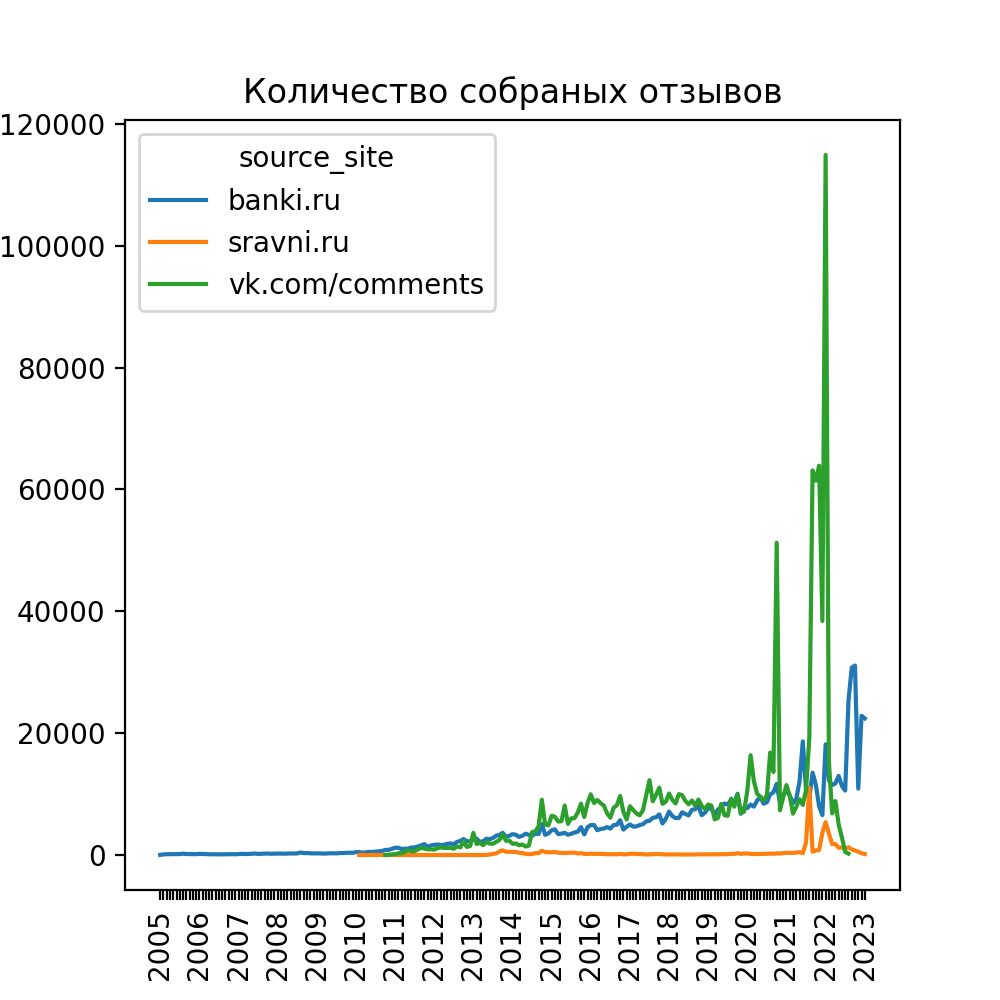
\includegraphics[width=0.6\textwidth]{img/reviews_count.png}
\caption{\label{fig:collected_data}График собранных предложений}
\end{figure}

\begin{figure}[h!]
\centering
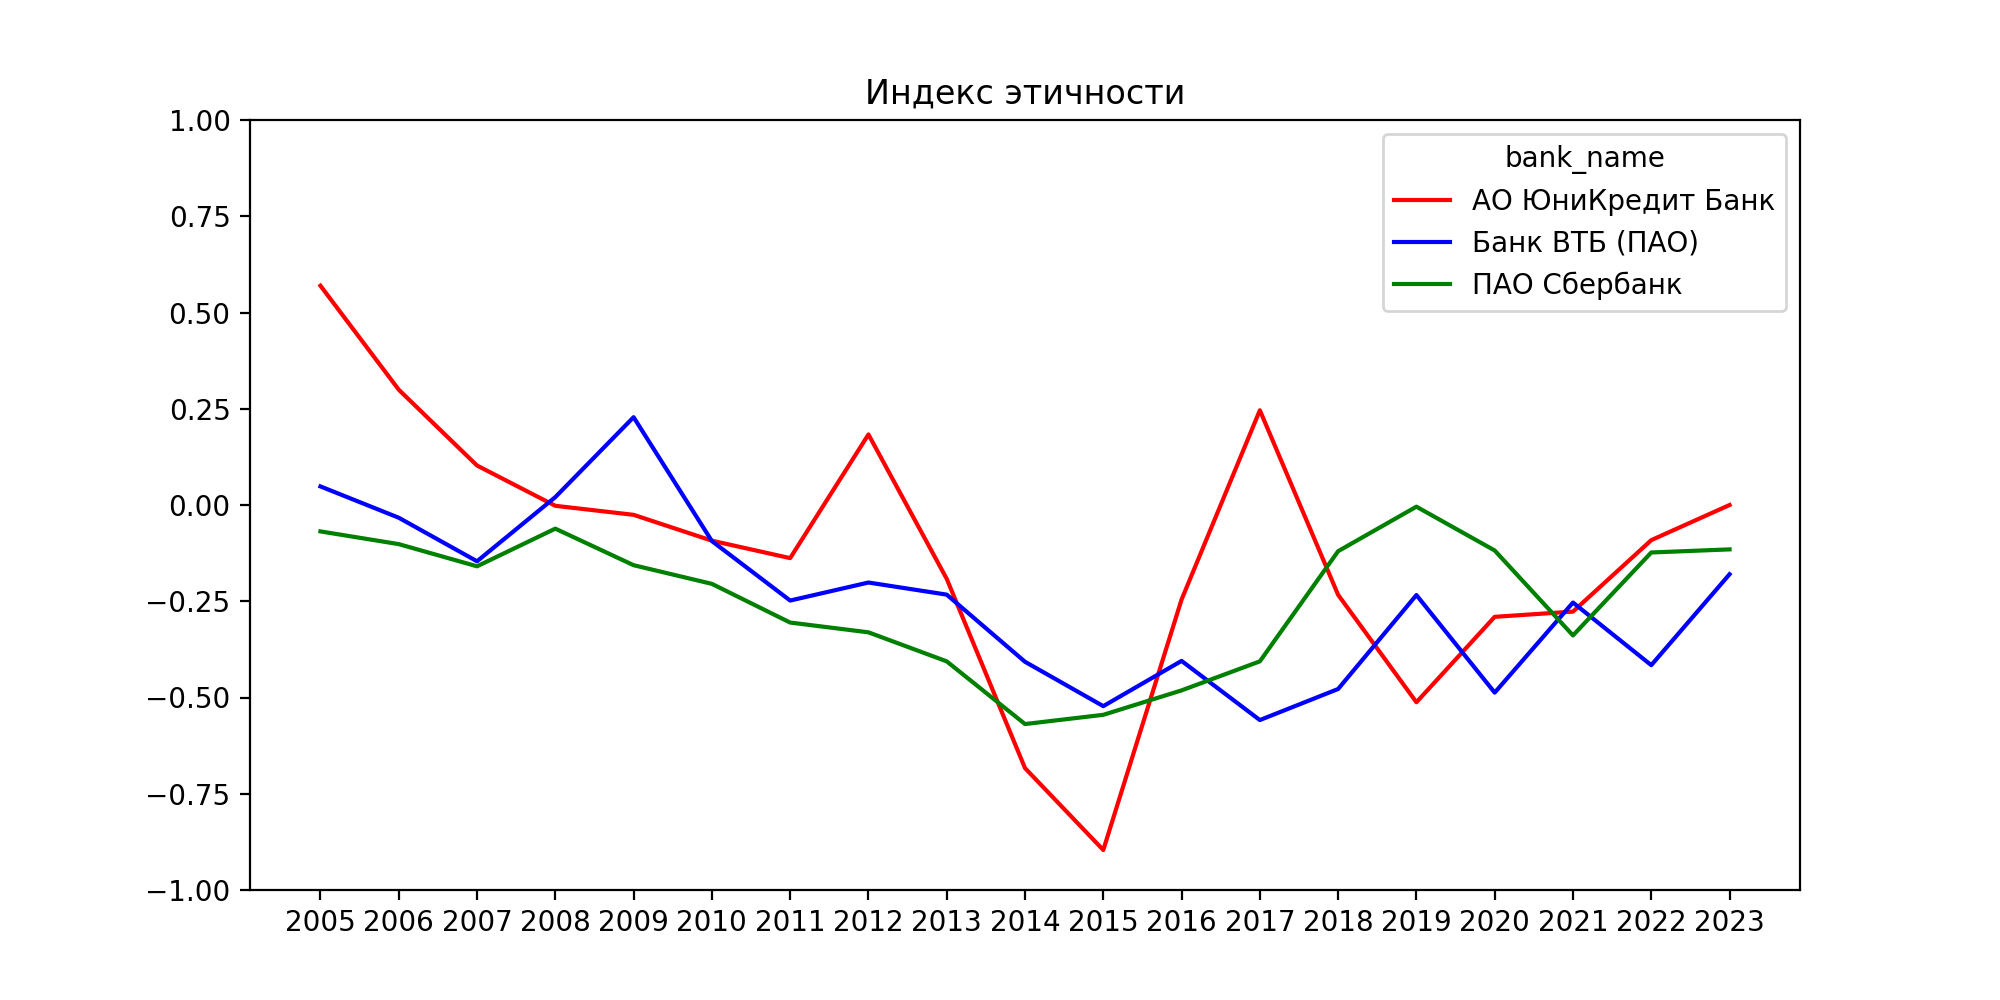
\includegraphics[width=0.8\textwidth]{img/ethics_plot_index_safe.png}
\caption{\label{fig:ethics_analisys}График оценки этичности компаний}
\end{figure}
\chapter{Тестирование системы}
\label{sec:org8876b0c}
В данной главе описывается разные методы тестирования, которые были использованы при реализации системы и форматтеры кода и инструменты статического анализа также является важным, поскольку это позволяет снизить количество ошибок и повысить качество кода.
\section{Форматирование кода}
\label{sec:orgcb243ca}
Во время реализации системы использовались различные инструменты для форматирования кода и обеспечения его качества, такие как black, isort, pyupgrade, flake8 и mypy.

Black — это инструмент для автоматического форматирования кода на языке программирования Python. Он помогает унифицировать стиль кодирования и повысить читаемость программного кода. Black применяет строгий набор правил форматирования, основанный на принципах PEP 8, и автоматически применяет эти правила к коду. Таким образом, он обеспечивает согласованность форматирования в проекте и упрощает совместную работу между разработчиками.

Isort — это инструмент для автоматической сортировки импортов в коде на языке Python. Он обеспечивает единообразное расположение импортов, что способствует повышению читаемости кода и уменьшению вероятности возникновения конфликтов и ошибок, связанных с порядком импорта модулей. Isort анализирует импорты в коде и автоматически сортирует их в соответствии с определенными правилами, такими как сортировка по имени модуля или по группам.

Pyupgrade представляет собой программный инструмент, предназначенный для автоматического обновления кода на языке Python до более новых версий данного языка. Такое обновление обеспечивает возможность использования новейших функциональных возможностей и улучшений, внедренных в последних версиях Python, а также элиминирует устаревшие конструкции и библиотеки. Путем проведения анализа исходного кода, Pyupgrade осуществляет автоматическое внесение изменений, таких как замена устаревших конструкций и актуализация синтаксиса, в соответствии с более современными стандартами языка.

Flake8 — это инструмент для обнаружения синтаксических и стилистических ошибок в коде на языке Python. Он выполняет статический анализ и проверяет код на соответствие стандартам кодирования и рекомендациям PEP 8. Flake8 выдает предупреждения и ошибки при обнаружении неправильного форматирования, несоответствия стилю кодирования или использования нежелательных конструкций. Это помогает улучшить качество кода, облегчает его понимание и уменьшает возможность возникновения ошибок.

Mypy представляет собой инструмент статического анализа кода на языке Python, призванный обнаруживать ошибки еще на этапе разработки. Путем проверки типов переменных, аргументов функций и других типовых аннотаций, указанных в исходном коде, Mypy способен выявить ошибки и предупредить об их наличии в случае несоответствия типов данных ожидаемым. Это позволяет предотвратить множество ошибок, связанных с типизацией данных, еще до запуска программы, что повышает надежность кода и облегчает его поддержку.

Также для автоматического форматирования кода использовался инструмент pre-commit, который позволяет форматировать кодовую базу перед отправкой в репозиторий с кодом.
\section{Тестирование системы}
\label{sec:org8d526c9}
Для тестирования системы были написаны скрипты Github actions, которые запускали тестирование системы при отправки кода в репозиторий. Для тестирования использовалась библиотека pytest \autocite{krekel_pytest_2004}, также для анализа покрытия кода использовалась библиотека \texttt{pytest-cov}.
\subsection{Тестирование модуля работы с базой данных}
\label{sec:org35d93be}
При запуске каждого теста создавалась новая база данных и к ней применялись миграции. В зависимости от нужного теста в базу данных помещались нужные данные. Каждый метод API тестировался на верные данные, не верные данные и пустые данные, затем проверялось, что записалось в базу данных. В зависимости от требований каждого теста в базу данных помещались соответствующие данные. Затем создавался клиент для тестирования API с помощью библиотеки httpx.

Для каждого метода API тестировалось его поведение на правильные, неправильные и пустые данные. Затем проверялось, что записалось в базу данных и соответствует ожиданиям.

\begin{figure}[h]
\centering
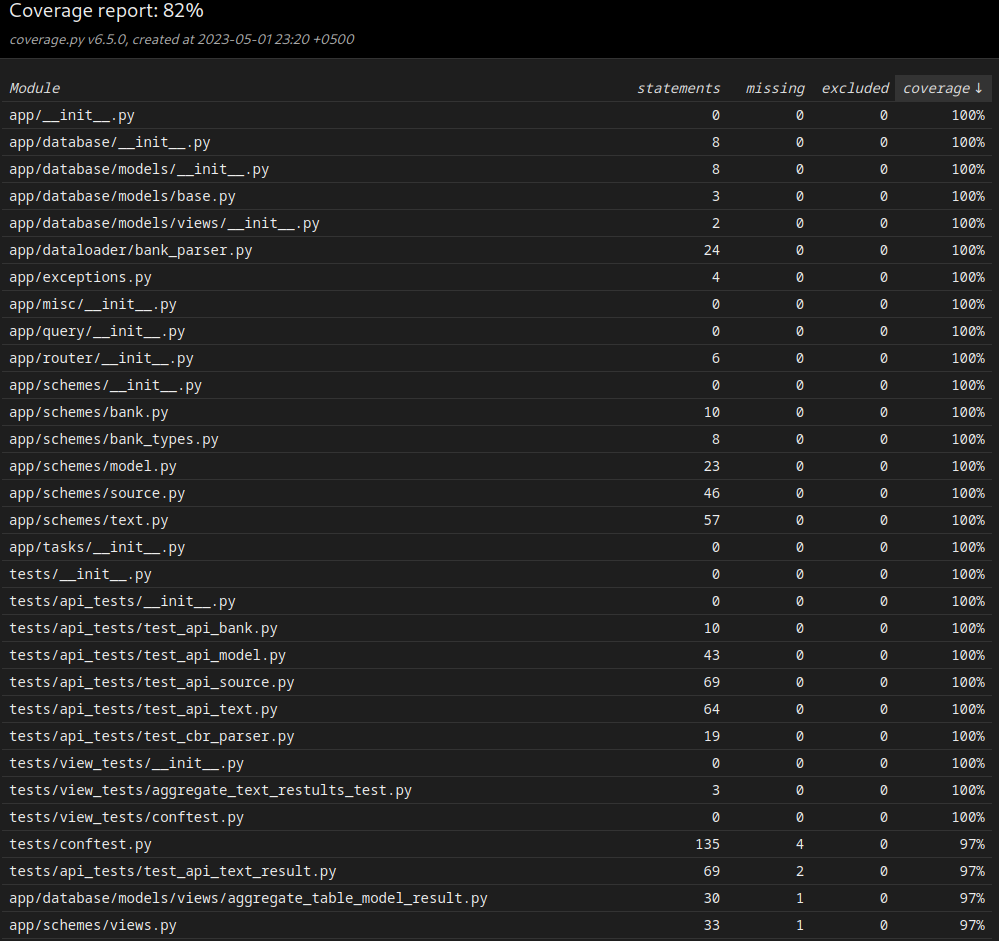
\includegraphics[width=0.8\textwidth]{img/api_coverage.png}
\caption{\label{fig:api_coverage}Покрытие кода модуля работы с базой данных тестами}
\end{figure}
\subsection{Тестирование модуля сбора данных}
\label{sec:org7cf65ac}
Тестирование сборщиков данных заключается в проверке корректности извлечения и обработки данных, получаемых из HTML-страниц и json. Также важно проверять сбор данных на актуальных данных сайтов. Для имитации запросов к API и сайтам использовалась библиотека requests-mock, для сохранения данных страниц использовалась библиотека \texttt{vcrpy}. Данная библиотека при первом запросе сайта сохраняет данные запроса (заголовки, параметры и так далее), а тело запроса кодирует в байты, что позволяет сократить объем. При последующих запросов вместо реального ответа будут подставляться данные предыдущего ответа. Такой способ работы с запросами позволяет ускорить процесс тестирования. Также при запуске каждого теста создавалась новая база данных.

При написании тестирования были реализованы mock-данные для API. Для подмены запросов на тестовые сначала делались запросы (или брались данные предыдущих запросов), затем с помощью библиотеки \texttt{requests-mock} данные запроса подменялись на тестовые. Потом запускались тесты, которые проверяли корректности работы функций.

\begin{figure}[h]
\centering
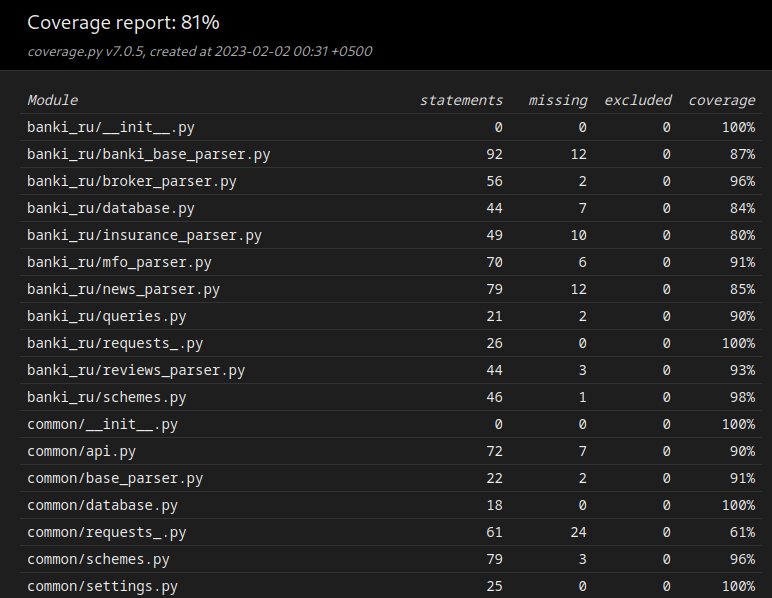
\includegraphics[width=0.8\textwidth]{img/parser_coverage.png}
\caption{\label{fig:parser_coverage}Покрытие кода модуля сборщиков данных тестами}
\end{figure}
\section{Выводы по главе}
\label{sec:orge0ac6c6}
В данной главе были описаны различные виды тестирования, которые использовались при тестировании модулей для работы базой данных и сбора данных.

Были описаны тесты для сборщиков данных, которые позволяют убедиться в корректности работы при различных сценариях. Также были рассмотрены тесты для HTTP API, которые проверяют работу API на правильную обработку запросов и на корректное взаимодействие с базой данных.
\chapter*{Заключение}
\label{sec:orgcb805c2}
В ходе анализа предметной области, была рассмотрена проблема определения этичности компаний и был произведен обзор существующих решений, который показал, что сейчас нет индекса, который бы учитывал мнение клиентов для анализа этичности, и может потребоваться разработка нового средства, учитывающего особенности задачи.

Было произведено изучение существующих исследований и работ по обработке естественного языка и оно показало, что в этой сфере применяется множество алгоритмов, такие как мешок слов, TF-IDF, Word2Vec, FastText и BERT и каждый из этих алгоритмов показал свою эффективность в различных сферах. Также для задач классификации были рассмотрены: логистическая регрессия, метод опорных векторов, случайный лес и градиентный бустинг. И они были также рассмотрены в этой работе.

Был произведен анализ требований, который в результате которого были определены необходимые функциональные и нефункциональные требования, которые будут учитывались при разработке решения. Все требования, выявленные в ходе анализа, были формализованы в техническом задании на разрабатываемую систему.

В ходе проектирования системы она была разбита на отдельные модули и было описано их взаимодействие. Каждый модуль был разработан с учетом принципов микросервисной архитектуры и обеспечивает функциональность, необходимую для реализации системы в целом.

Была спроектирована база данных для хранения информации об отзывах, источниках, моделях и компаниях  с учетом требований к масштабируемости и производительности системы.

Было проведено проектирование методов для лучшего подбора метода обработки текста и модели классификации. Для этого была подобрана метрика, которая позволит лучшим образом отразить результат подбора моделей.

При реализации поставленной задачи было проведено обучение алгоритмов обработки естественного текста и классификации и лучший результат дало сочетание моделей дообученного BERT с размороженными двумя слоями и логистической регрессии с метрикой F1 равной 0.83.

Также было собрано 2,5 миллиона отзывов о компаниях с разных сайтов и реализованы модули по обработке и работе с данными. Система была развернута с помощью docker-compose.

Было проведено тестирование модулей сбора и работы с данными с результатом покрытия 80\%.

В заключении можно отметить, что проект является успешным и достигнуты поставленные цели и задачи.

\putbibliography
\appendix
% https://www.swrit.ru/doc/gost34/34.602-2020.pdf
% Сделано по гост 34.602-2020
{ % чтобы в главном тексте не сбрасывались заголовки
%%%%%%%%%%%%%%%%%%%%% переопределение секций чтобы было 1.1. вместо А.1.1.
\renewcommand*{\thesection}{\arabic{section}}
\titleformat{\section}{\large\bfseries}{\thesection.}{4pt}{}

\renewcommand*{\thesubsection}{\arabic{section}.\arabic{subsection}}
\titleformat{\subsection}{\large\bfseries}{\thesubsection.}{4pt}{}

\renewcommand*{\thesubsubsection}{\arabic{section}.\arabic{subsection}.\arabic{subsubsection}}
\titleformat{\subsubsection}{\normalsize\bfseries}{\thesubsubsection.}{4pt}{}
\setcounter{secnumdepth}{4}

%%%%%%%%%%%%%%%%%%%%%%%%%% 5
{ % для титульного листа
  \chapter*{ПРИЛОЖЕНИЕ А Техническое задание на разрабатываемую систему}\label{tz_chap}

\stepcounter{chapter}
\thispagestyle{empty}
\centering

\begin{flushright}
  \MakeUppercase{Утверждено}

  A.B.00001-01 ТЗ 01
\end{flushright}

\vfill

\textbf{\MakeUppercase{Система для автоматического сбора, анализа и визуализации информации по этичности компаний}}

\textbf{Техническое задание}

\textbf{\textit{Лист утверждения}}

\vbox{
  \parbox{6cm}{
    \begin{sideways}
      \setlength\arrayrulewidth{2pt}
      \begin{tabular}{|c|c|c|c|c|}
        \hline
        Инв. № подл. & Подпись и дата & Взам. инв. № & Инв. № дубл. & Подпись и дата \\
        \hline
                     &&&&\\
        \hline
      \end{tabular}
    \end{sideways}
  }
  \hfill
  \parbox{9.4cm}{
    \begin{flushright}
      \begin{minipage}[t]{0.4\textwidth}
        Руководитель разработки

        \vspace{3mm}
        \makebox[6cm][r]{\hrulefill~Бузмаков~А.В.}
        \makebox[6cm][r]{<<\rule{7mm}{0.4pt}>>\hrulefill~\the\year}
      \end{minipage}
    \end{flushright}
    \vspace{10mm}
    \begin{flushright}
      \begin{minipage}[t]{0.4\textwidth}
        Исполнитель

        \vspace{3mm}
        \makebox[6cm][r]{\hrulefill~Соломатин~Р.И.}
        \makebox[6cm][r]{<<\rule{7mm}{0.4pt}>>\hrulefill~\the\year}
      \end{minipage}
    \end{flushright}
  }
}
\newpage
}
\section{Общие сведения}
Наименование программы – <<Система для автоматического сбора, анализа и визуализации информации по этичности компаний>> (далее – <<Система>>). Основная функция системы - сбор и анализ данных из различных источников, включая новостные сайты, социальные сети, отзывы о компаниях и другие открытые источники данных. Система использует алгоритмы машинного обучения и обработки естественного языка для автоматической обработки данных и определения этичности компаний.

Система также предоставляет визуализацию данных в виде графиков и диаграмм, позволяя пользователям легко понять и сравнивать данные по разным компаниям. Кроме того, система может предоставлять аналитические отчеты и рекомендации по улучшению этичности компаний на основе собранных данных.

Система разрабатывается в рамках выполнения выпускной квалификационной работы. Основанием для разработки являются:
\begin{itemize}
  \item Положение о курсовой и выпускной квалификационной работе студентов, обучающихся по программам бакалавриата, специалитета и магистратуры в Национальном исследовательском университете <<Высшая школа экономики>>, утвержденным ученым советом НИУ ВШЭ (протокол от 28.11.2014 № 08), с изменениями от 29.03.2016;
  \item Правила подготовки выпускной квалификационной работы студентов основной образовательной программы бакалавриата <<Программная инженерия>> по направлению подготовки 09.03.04. Программная инженерия, утвержденные протоколом ученого совета НИУ ВШЭ – Пермь от 19.11.2020 № 8.2.1.7-10/10.
\end{itemize}

\section{Цели и назначение создания автоматизированной системы}

\subsection{Цели создания АС}
Целью создания системы является получение инструмента который позволит анализировать компании на основании их этичности, соответствующего следующим требованиям:
\begin{itemize}
  \item Показывать историю изменений индекса с возможностью фильтровать по
        \begin{itemize}
          \item годам;
          \item отраслям компаний, с возможностью множественного выбора;
          \item компаниям, с возможностью множественного выбора;
          \item моделям, с возможностью множественного выбора;
          \item источникам, с возможностью множественного выбора.
        \end{itemize}
  \item Агрегировать значения индекса по годам и кварталам;
  \item Анализировать тексты для построения индекса этичности;
  \item Иметь возможность добавления анализа текста несколькими вариантами;
  \item Сохранять тексты для последующего анализа другими методами;
  \item Система должна собирать данные с сайтов banki.ru, sravni.ru и комментарии из групп {}<<вконтаке>>{};
  \item На сайте должен быть график, который показывать изменение индекса этичности компаний и количества собранных отзывов по разным источникам.
  \item Для расчета индекса этичности компаний на основании рецензий должна использоваться формула\ref{eq:ethics_tz}:
        \begin{equation}
          \label{eq:ethics_tz}
          \begin{aligned}
            \text{Base index} &= \frac{\text{positive} - \text{negative}}{\text{positive} + \text{negative}} \\
            \text{Std index} &= \sqrt{\frac{\text{positive}}{\text{negative} \cdot (\text{positive} + \text{negative})^{3}} + \frac{\text{negative}}{\text{positive} \cdot (\text{positive} + \text{negative})^{3}}} \\
            \text{Index} &= ({2\cdot({\text{Base index}}-{\text{Mean index}} > 0) - 1})\cdot\\
                              &{max\left(\left|{\text{Base index}}-{\text{Mean index}}\right|-{\text{Std index}}, 0\right)}
          \end{aligned}
        \end{equation}

        \(positive\) -- количество позитивных предложений,

        \(negative\) -- количество негативных предложений,

        \(Mean\ index\) -- среднее значения для пар источник сбора данных и модели, которая обрабатывала предложения.
\end{itemize}


\subsection{Назначение АС}
Система предназначена для собора и анализа отзывы потребителей с различных веб-сайтов, с помощью алгоритмов обработки естественного языка.
\section{Характеристика объекта автоматизации}
Система автоматизирует процесс анализа этичности компаний.
\section{Требования к автоматизированной системе}
Требования к АС:
\begin{enumerate}
  \item построение графика не должно занимать больше секунды;
  \item данные должны собираться автоматически;
  \item данные должны обрабатываться автоматически;
  \item система должны способна работать с большим объемом информации;
  \item система должна быть стабильна.
\end{enumerate}
\subsection{Требования к структуре АС в целом}
Должно быть несколько модулей, которые общаются между собой с помощью HTTP API:
\begin{itemize}
  \item сборщики данных;
  \item взаимодействие с базой данных(API);
  \item сайт;
  \item модели для обработки данных.
\end{itemize}
Все подсистемы должны быть в Docker контейнерах.
\subsection{Требования к функциям (задачам), выполняемым АС}
\subsubsection{Требования к API}
Система взаимодействия с базой данных должна выполнять функции:
\begin{itemize}
  \item хранить информацию о компаниях;
  \item модель должна отдавать информацию о компаниях из разных сфер;
  \item хранить информацию о разных источниках;
  \item добавлять различные источники;
  \item получать отзывы и разбивать их на предложения;
  \item иметь возможность отдавать необработанные предложения в зависимости от модели;
  \item сохранять информацию о моделях;
  \item сохранять результат обработки предложений;
  \item агрегировать результат обработки моделей для каждого квартала;
  \item хранить информацию о состоянии сборщиков данных, если у них возникнут проблемы;
  \item отдавать информацию об индексе менее, чем за минуту;
  \item рассчитывать индекс на основе полученных результатов обработки предложений.
\end{itemize}
\subsubsection{Требования к сборщикам данных}
Сборщики данных должны выполнять функции:
\begin{itemize}
  \item собирать отзывы пользователей ежедневно;
  \item собранные отзывы отправлять на API.
\end{itemize}
\subsubsection{Требования к моделям}
Модели должны выполнять функции:
\begin{itemize}
  \item обрабатывать отзывы пользователей ежедневно;
  \item обработанные отзывы отправлять на API.
\end{itemize}
\subsection{Требования к видам обеспечения АС}
\subsubsection{Требования к лингвистическому обеспечению}
Система должна соответствовать следующим требованиям:
\begin{itemize}
  \item Программный код должен быть реализован на языке Python;
  \item Документация к программе должна быть на русском языке. Других языков не планируется.
\end{itemize}
\subsubsection{Требования к программного обеспечению}
Система должна использовать:
\begin{itemize}
  \item Для разработки API следует использовать библиотеку FastAPI;
  \item Для взаимодействия с базой данных должна использоваться библиотека SQLAlchemy, а для миграций Alembic;
  \item Сборщики данных должны собирать информацию с помощью библиотеки запросов
        requests и для работы с HTML Beautiful Soup;
  \item Для нейросетевых моделей должен использоваться Pytorch;
  \item Для клиентской части будет использоваться библиотека React.
\end{itemize}
\subsubsection{Требования к техническому обеспечению}
Для работы приложения необходим сервер, который обладает следующими параметрами:
\begin{itemize}
  \item Процессор с тактовой частотой не ниже 3 ГГц и 8 ядрами;
  \item Операционная система Ubuntu 22.04 и выше;
  \item Docker 20.10.23 и выше.
  \item Графическая карта NVIDIA GTX 3080;
  \item Оперативная память не менее 16 Гб;
  \item Доступное место на жестком диске не менее 100 Гб;
\end{itemize}
\subsubsection{Требования к информационному обеспечению}
Система должна соответствовать следующим требованиям:
\begin{itemize}
  \item Система должна использовать PostgreSQL;
  \item Сервисы между собой должны взаимодействовать при помощи HTTP;
  \item Для базы данных должен всегда быть резервная копия данных.
\end{itemize}

\subsection{Общие технические требования к АС}
\subsubsection{Требования к численности и квалификации персонала}
Для разработки системы требуется программист со средней квалификацией. Для
работы с конечной системой (сайтом), не требуется высокой квалификации, поэтому
пользователь с ней справится пользователь, который пользуется сайтами.
\subsubsection{Требования к надежности}
Надежность системы зависит от надежности функционирования сервера. Устойчивое
функционирование программы будет обеспечено с помощью:
\begin{itemize}
  \item Бесперебойное питание сервера;
  \item Использованием лицензионного программного обеспечения, необходимого для
        запуска приложения, включая лицензионную операционную систему;
  \item Регулярным выполнением рекомендаций Министерства труда и социального развития РФ, изложенных в Постановлении от 23 июля 1998 г. <<Об утверждении межотраслевых типовых норм времени на работы по сервисному обслуживанию ПЭВМ и оргтехники и сопровождению программных средств>>;
  \item Регулярным выполнением требований ГОСТ 51188-98 <<Защита информации. Испытания программных средств на наличие компьютерных вирусов>>;
\end{itemize}
Время восстановление системы будет до 10 минут с момента сбоя.
\subsubsection{Требования по сохранности информации при авариях}
Отказы как самой системы, так и ее отдельных функций, могут привести к
аварийному завершению работы программы, однако при перезапуске программы ее
функциональность не должна пострадать. При таких сбоях программы база данных не
должна пострадать. Дополнительно все данные будут резервно копироваться на дополнительную базу данных.
\section{Состав и содержание работ по созданию автоматизированной системы}
\begin{longtblr}
  [caption={Этапы реализации, контрольные точки проекта},]
  {
    colspec = {|X|X|X|},
    rowhead = 1,
    hlines,
  }
  % BEGIN RECEIVE ORGTBL stages
\textbf{Основной этап} & Подэтап & \textbf{Крайний срок}\\[0pt]
Анализ & Литературный обзор & 26.12.2022\\[0pt]
Анализ & Сравнительный анализ существующих решений & 08.01.2023\\[0pt]
Анализ & Анализ сценариев использования & 14.01.2023\\[0pt]
Анализ & Написание тех задания & 21.01.2023\\[0pt]
Проектирование & Проектирование архитектуры приложения & 14.02.2023\\[0pt]
Проектирование & Проектирование базы данных & 20.03.2023\\[0pt]
Проектирование & Проектирование графического интерфейса & 20.03.2023\\[0pt]
Проектирование & Проектирование алгоритмов машинного обучения & 20.03.2023\\[0pt]
Разработка & Разработка алгоритмов для анализа текста & 01.05.2023\\[0pt]
Разработка & Реализация серверной части & 01.05.2023\\[0pt]
Разработка & Реализация клиентской части & 01.05.2023\\[0pt]
Тестирование & Подготовка тестовых сценариев & 15.05.2023\\[0pt]
Тестирование & Функциональное тестирование & 15.05.2023\\[0pt]
Тестирование & Системное тестирование & 15.05.2023\\[0pt]
Завершение & Сдача проекта & 22.05.2023\\[0pt]
% END RECEIVE ORGTBL stages
\end{longtblr}
\begin{comment}
  #+ORGTBL: SEND stages orgtbl-to-latex
  | *Основной этап* | Подэтап                                      | *Крайний срок* |
  | Анализ          | Литературный обзор                           |     26.12.2022 |
  | Анализ          | Сравнительный анализ существующих решений    |     08.01.2023 |
  | Анализ          | Анализ сценариев использования               |     14.01.2023 |
  | Анализ          | Написание тех задания                        |     21.01.2023 |
  | Проектирование  | Проектирование архитектуры приложения        |     14.02.2023 |
  | Проектирование  | Проектирование базы данных                   |     20.03.2023 |
  | Проектирование  | Проектирование графического интерфейса       |     20.03.2023 |
  | Проектирование  | Проектирование алгоритмов машинного обучения |     20.03.2023 |
  | Разработка      | Разработка алгоритмов для анализа текста     |     01.05.2023 |
  | Разработка      | Реализация серверной части                   |     01.05.2023 |
  | Разработка      | Реализация клиентской части                  |     01.05.2023 |
  | Тестирование    | Подготовка тестовых сценариев                |     15.05.2023 |
  | Тестирование    | Функциональное тестирование                  |     15.05.2023 |
  | Тестирование    | Системное тестирование                       |     15.05.2023 |
  | Завершение      | Сдача проекта                                |     22.05.2023 |
\end{comment}

\section{Порядок разработки автоматизированной системы}
В разделе «Порядок разработки автоматизированной системы» приводят следующее:
\begin{itemize}
  \item порядок организации разработки АС;
  \item перечень документов и исходных данных для разработки АС;
  \item перечень документов, предъявляемых по окончании соответствующих этапов работ;
  \item порядок проведения экспертизы технической документации;
  \item перечень макетов (при необходимости), порядок их разработки, изготовления, испытаний, необходимость разработки на них документации, программы и методик испытаний;
  \item порядок разработки, согласования и утверждения плана совместных работ по разработке АС;
  \item порядок разработки, согласования и утверждения программы работ по стандартизации;
  \item требования к гарантийным обязательствам разработчика;
  \item порядок проведения технико-экономической оценки разработки АС;
  \item порядок разработки, согласования и утверждения программы метрологического обеспечения, программы обеспечения надежности, программы эргономического обеспечения.
\end{itemize}

\section{Порядок контроля и приемки автоматизированной системы}
Осуществление приемо-сдаточных испытаний для всей системы осуществляется на основе Программы и методики испытаний и включает:
\begin{itemize}
    \item Функциональное тестирование;
    \item Тестирование удобства эксплуатации;
    \item Оценка сгенерированных уровней.
\end{itemize}

\section{Требования к составу и содержанию работ по подготовке объекта автоматизации к вводу автоматизированной системы в действие}
\begin{longtblr}[caption={Требования к программной документации}]{colspec = {|X|X|},rowhead = 1,hlines,}
    \textbf{Название документа }          & \textbf{Краткое содержание} \\
    Текст программы \par(ГОСТ 19.401–78)  & Программный код всех модулей программы с необходимыми комментариями. \\
    Программа и методика испытаний \par(ГОСТ 19.301–79) & Требования, подлежащие проверке при испытании программы, а также порядок и методы их контроля. \\
    Техническое задание \par(34.602-2020) & Назначение и область применения программы, технические, технико-экономические и специальные требования, предъявляемые к программе, необходимые стадии и сроки разработки, виды испытаний. \\
\end{longtblr}
}

\chapter{Схема базы данных}
\label{sec:org3c996ea}
\begin{figure}[h!]
\centering
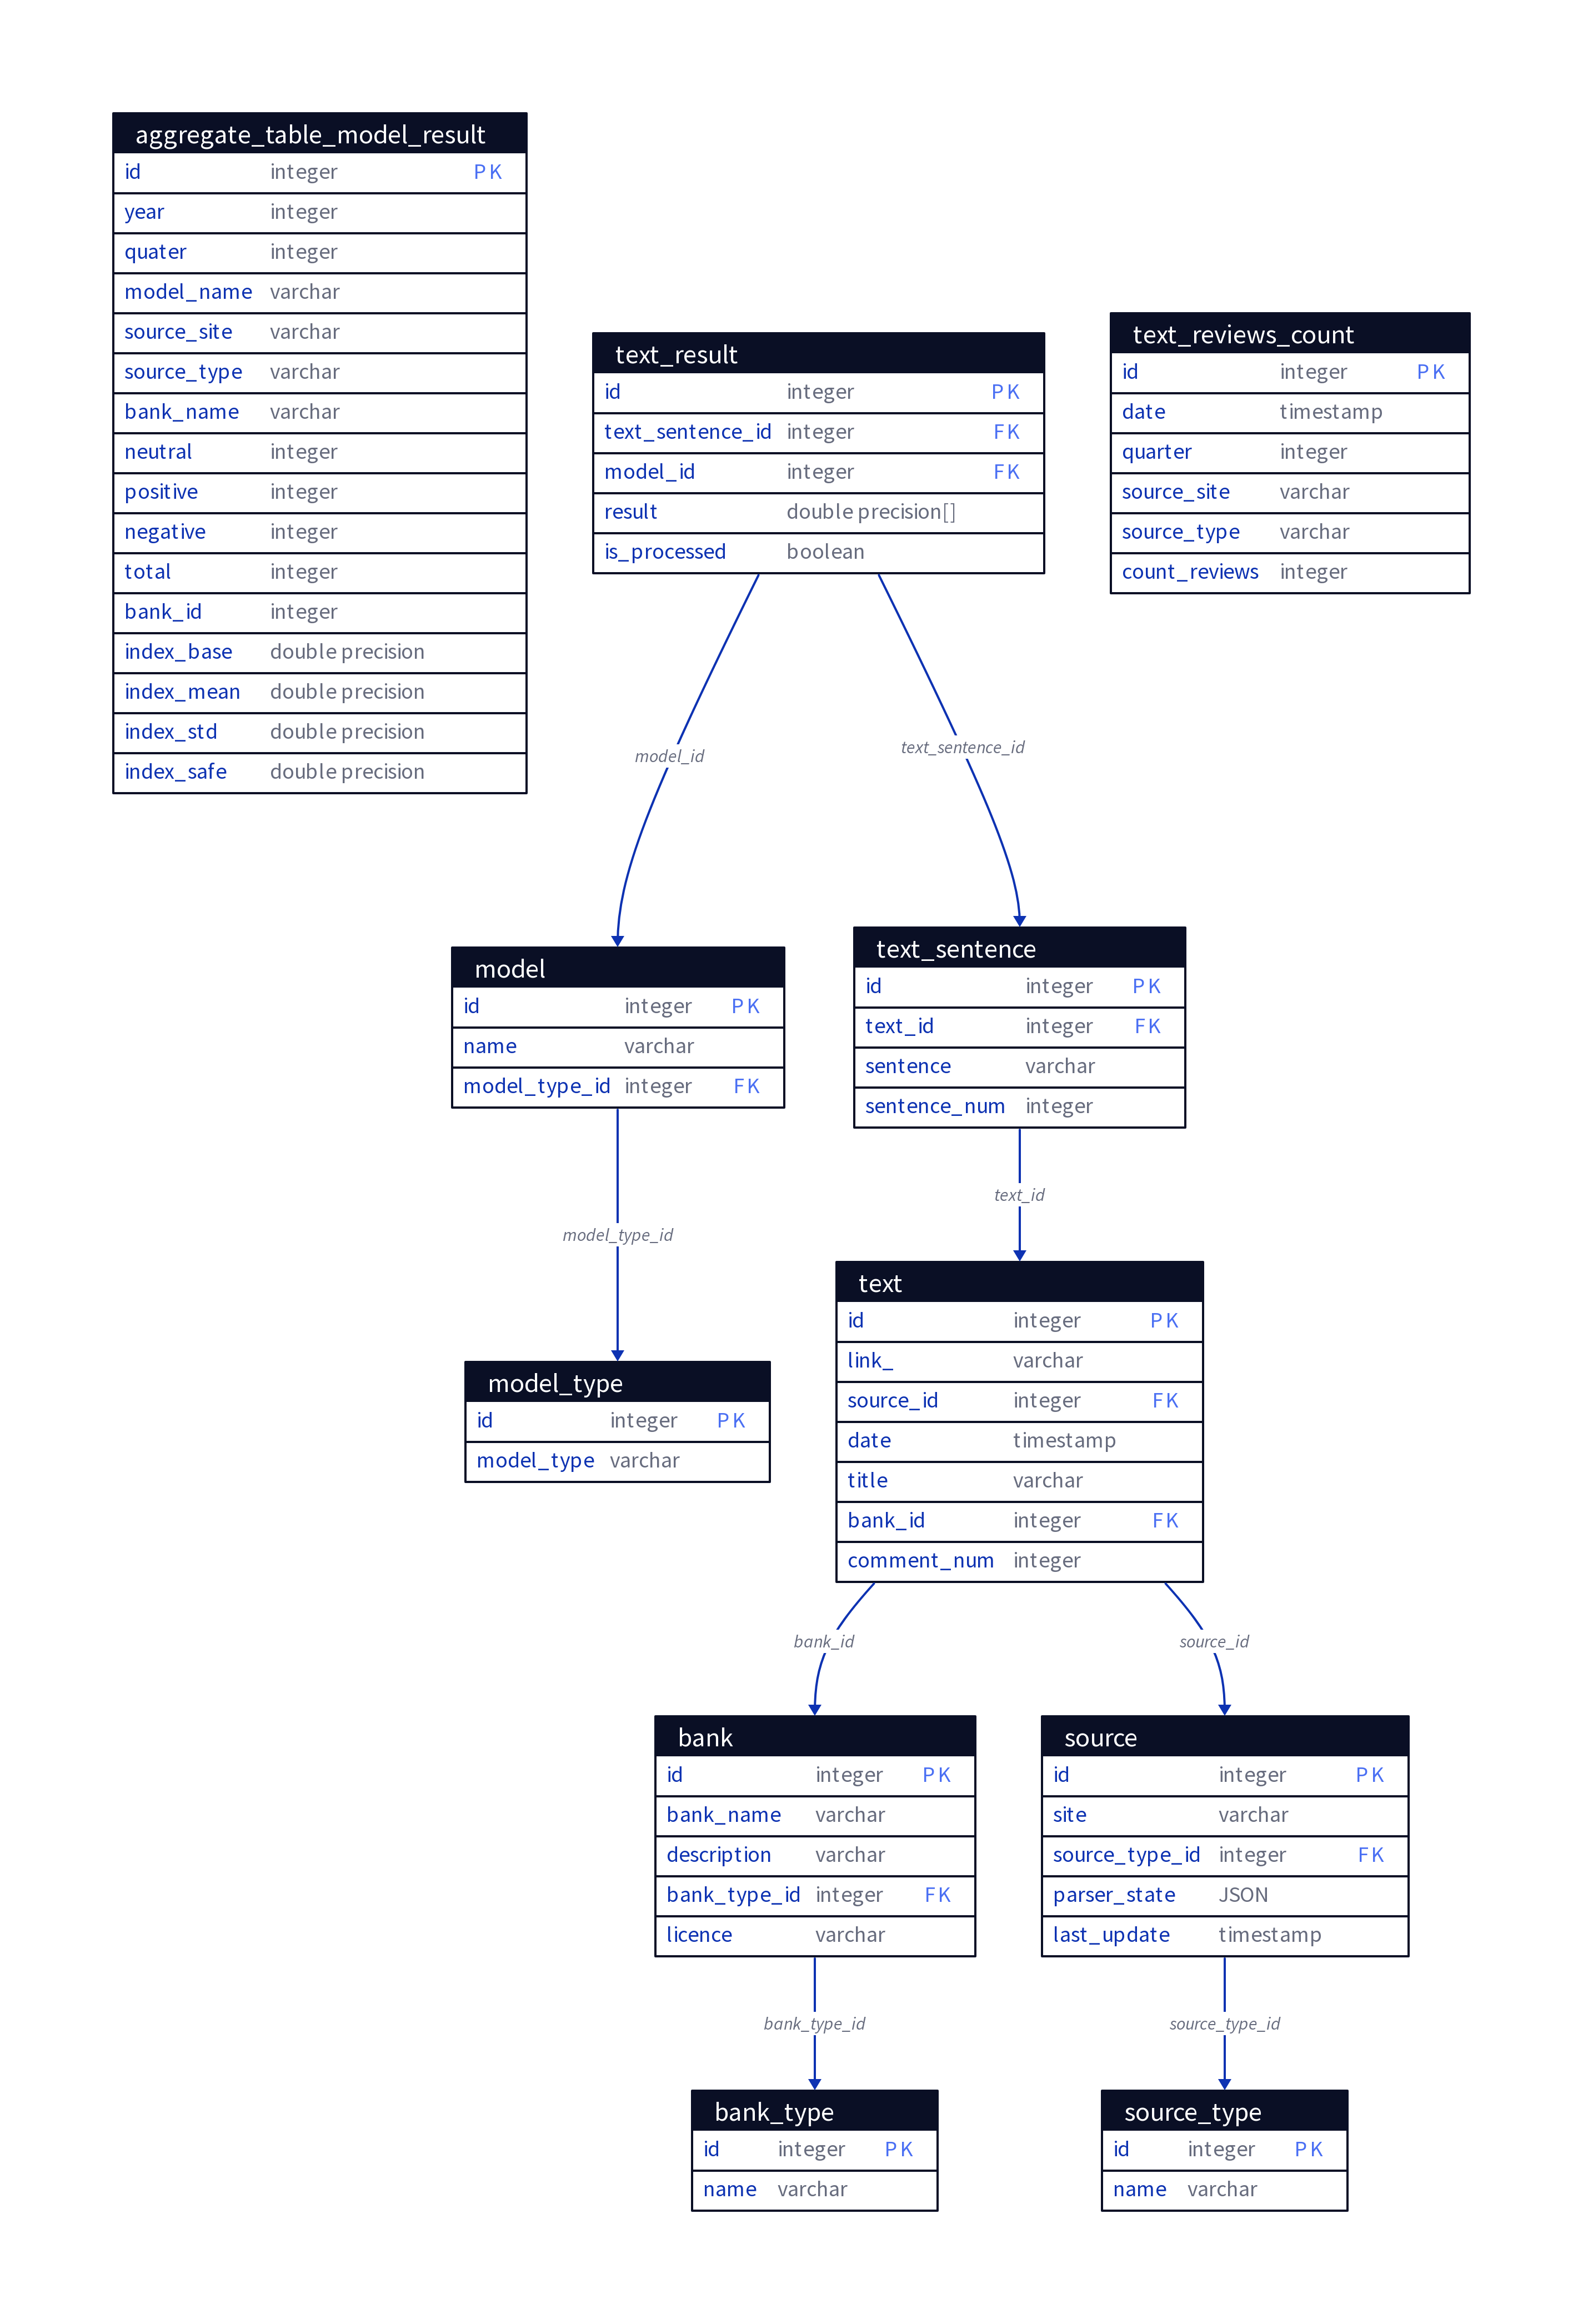
\includegraphics[width=0.8\textwidth]{img/d2/database.png}
\caption{\label{fig:database}Схема базы данных}
\end{figure}

\begin{figure}[h!]
\centering
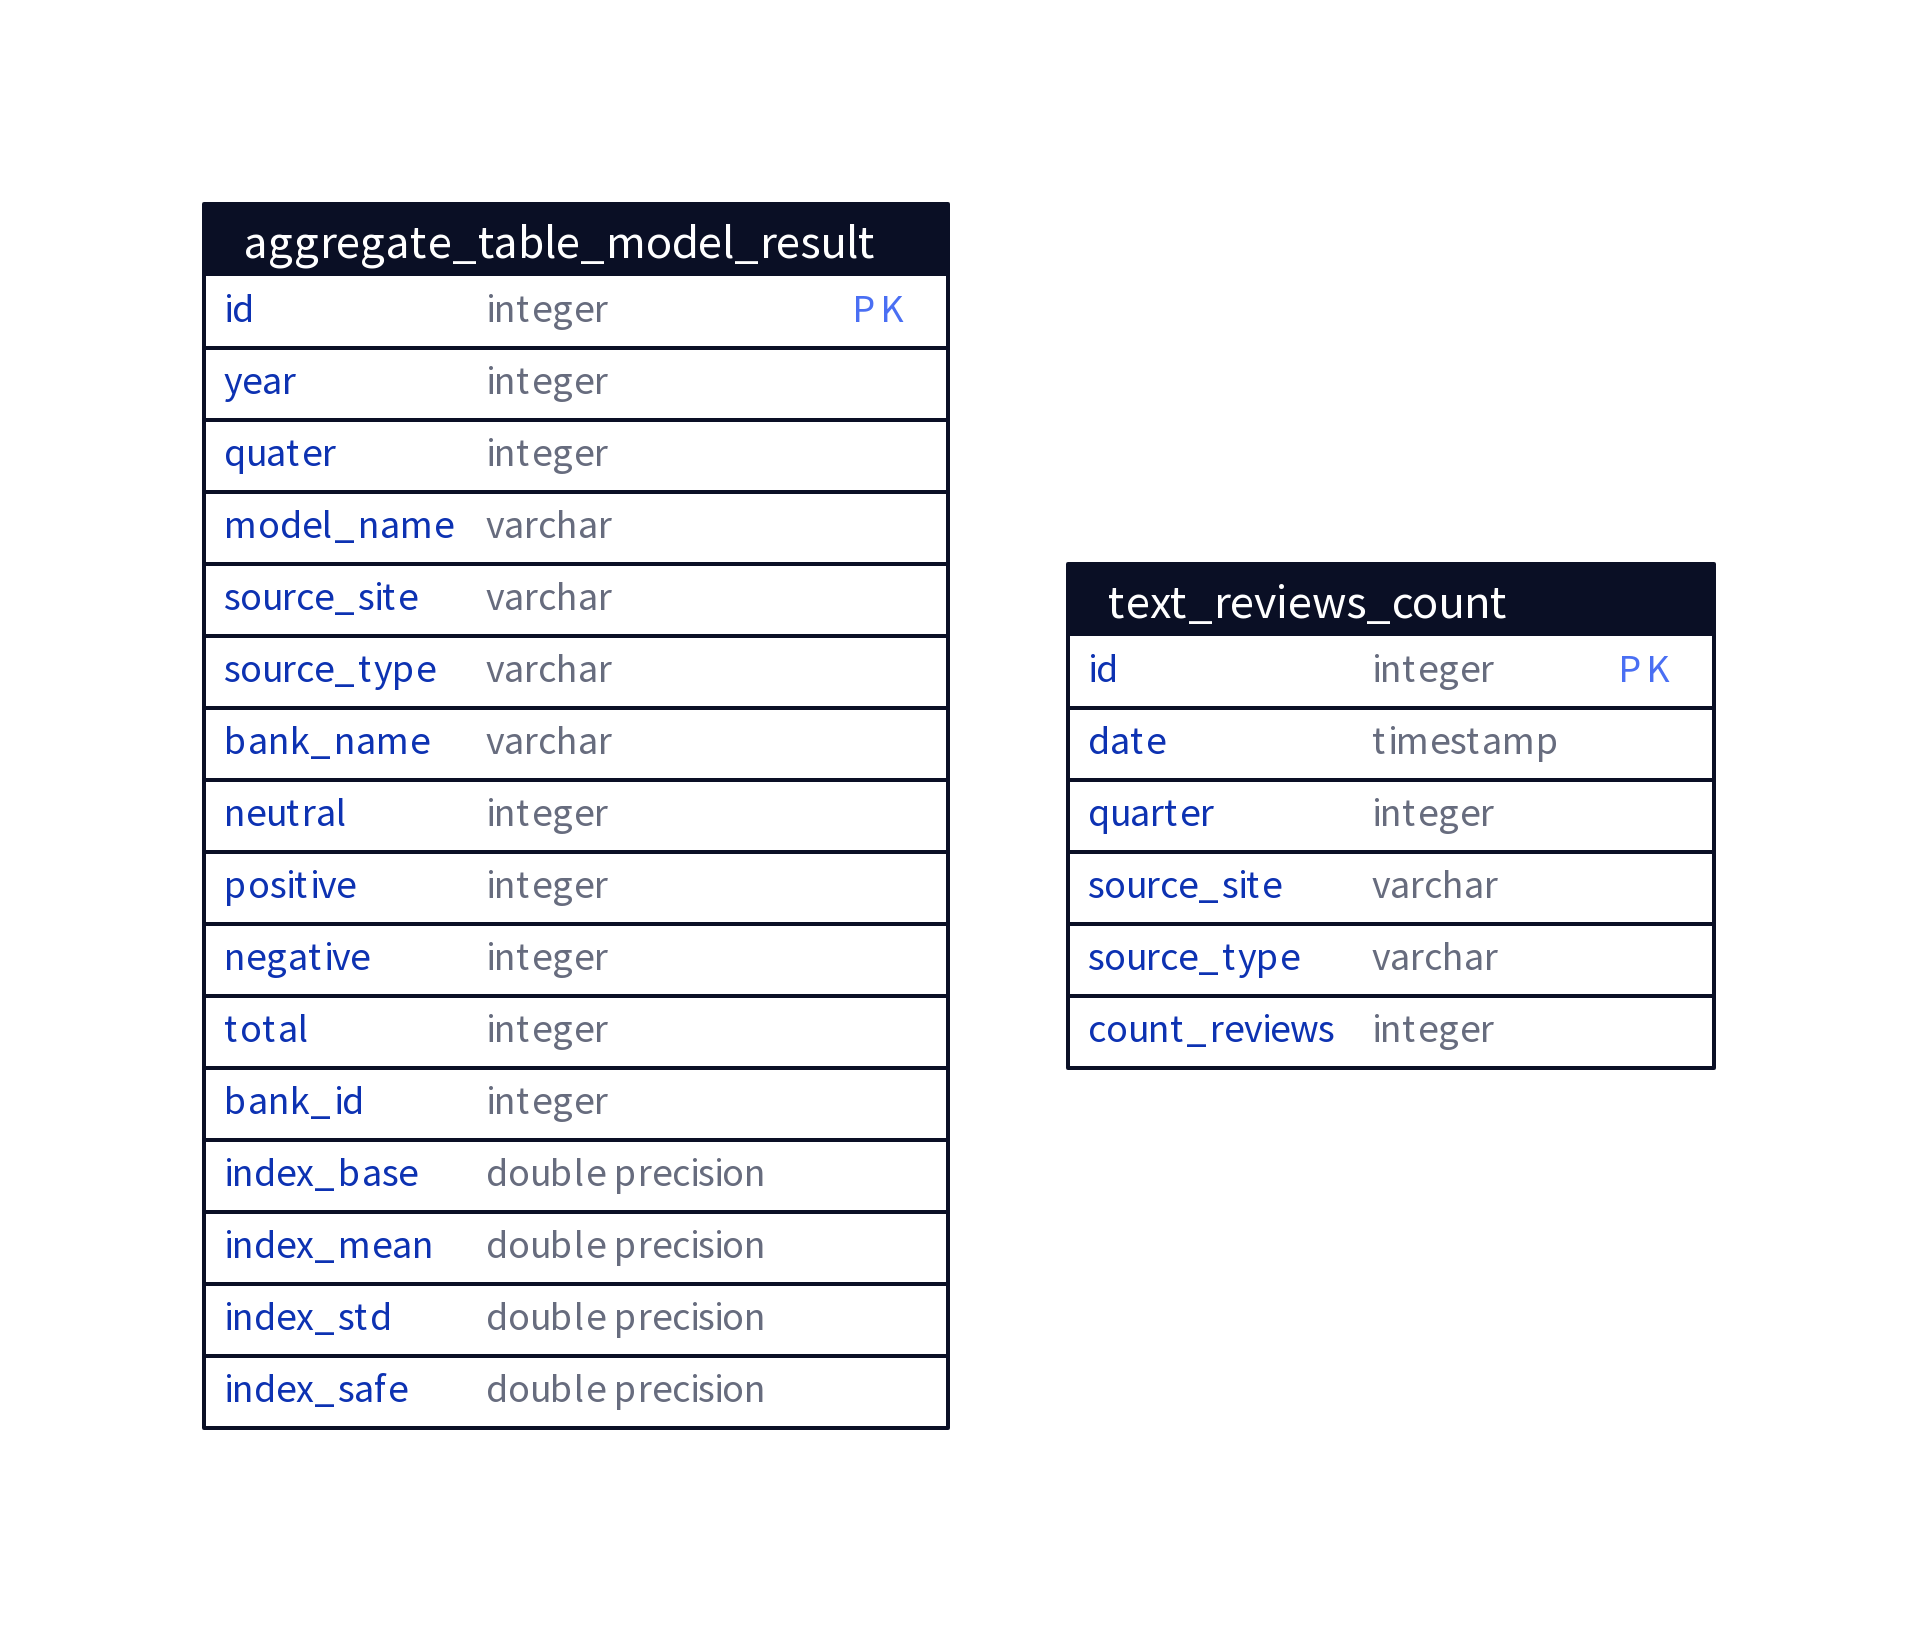
\includegraphics[width=0.8\textwidth]{img/d2/views_database.png}
\caption{\label{fig:database_views}Схема базы данных для агрегаций}
\end{figure}

\begin{figure}[h!]
\centering
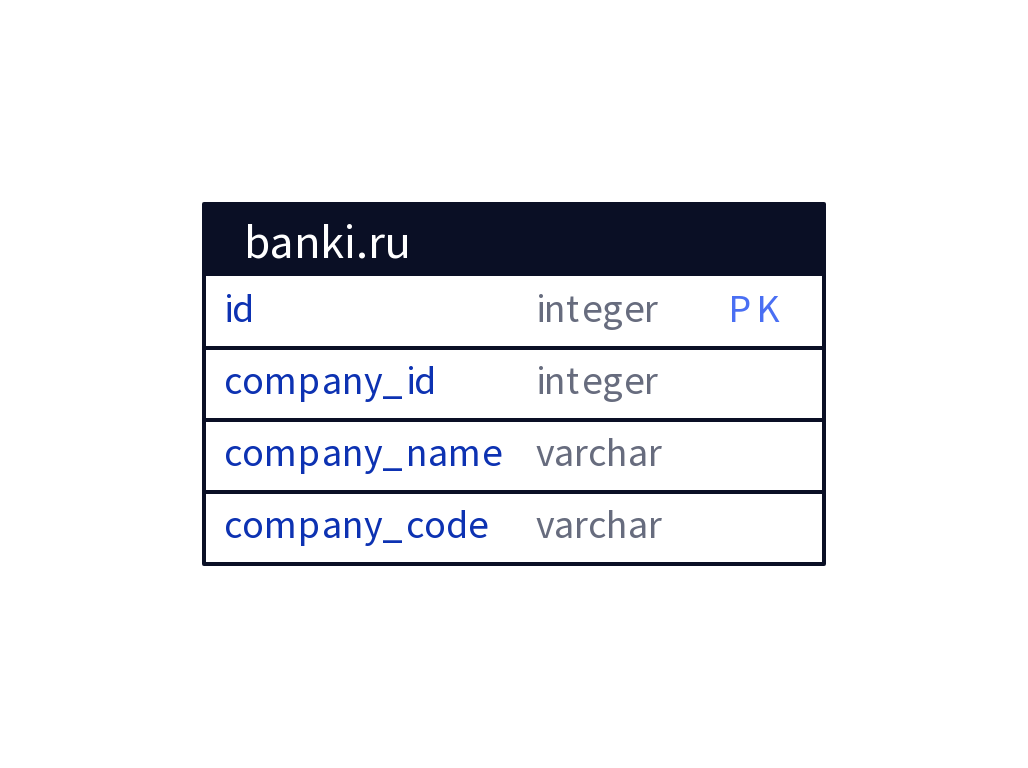
\includegraphics[width=0.8\textwidth]{img/d2/banki_ru.png}
\caption{\label{fig:database_banki_ru}Схема базы данных сайта banki.ru}
\end{figure}

\begin{figure}[h!]
\centering
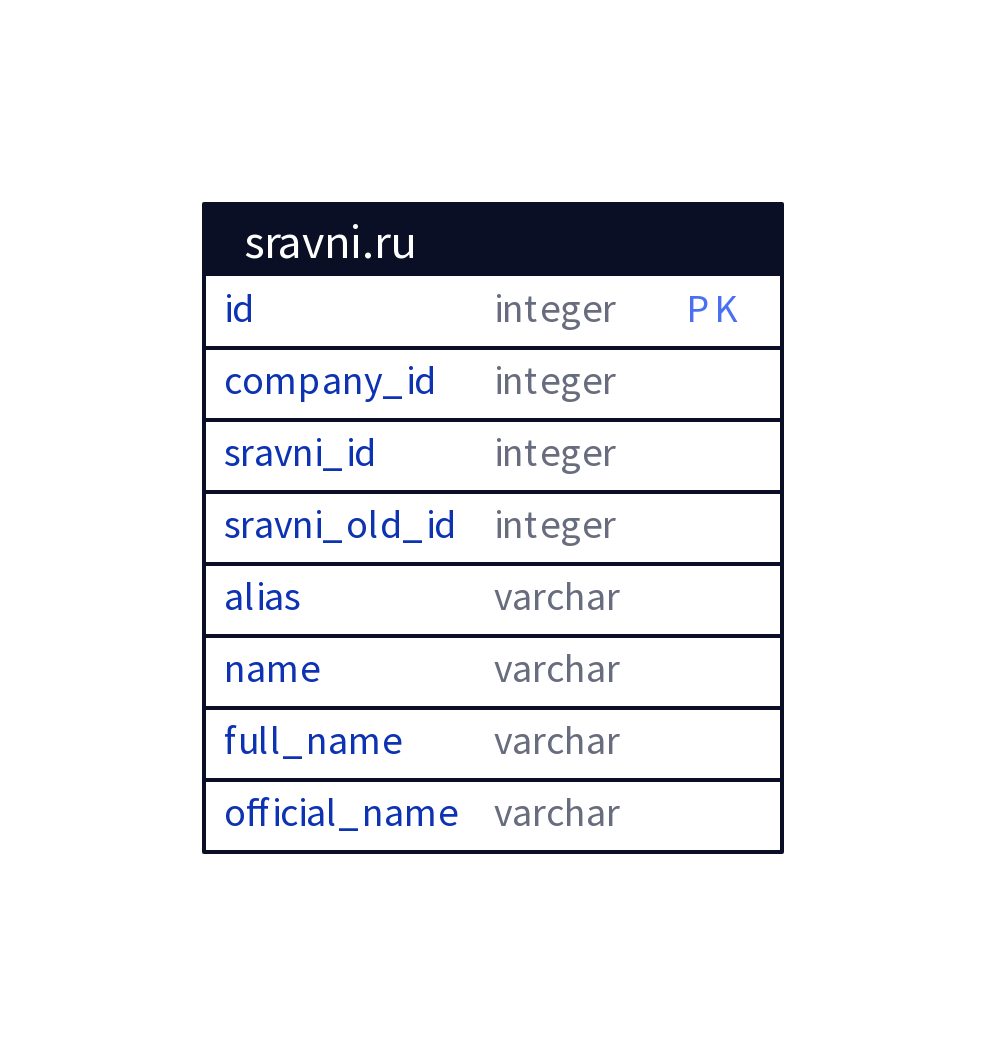
\includegraphics[width=0.8\textwidth]{img/d2/sravni_ru.png}
\caption{\label{fig:database_sravni_ru}Схема базы данных сайта sravni.ru}
\end{figure}

\begin{figure}[h!]
\centering
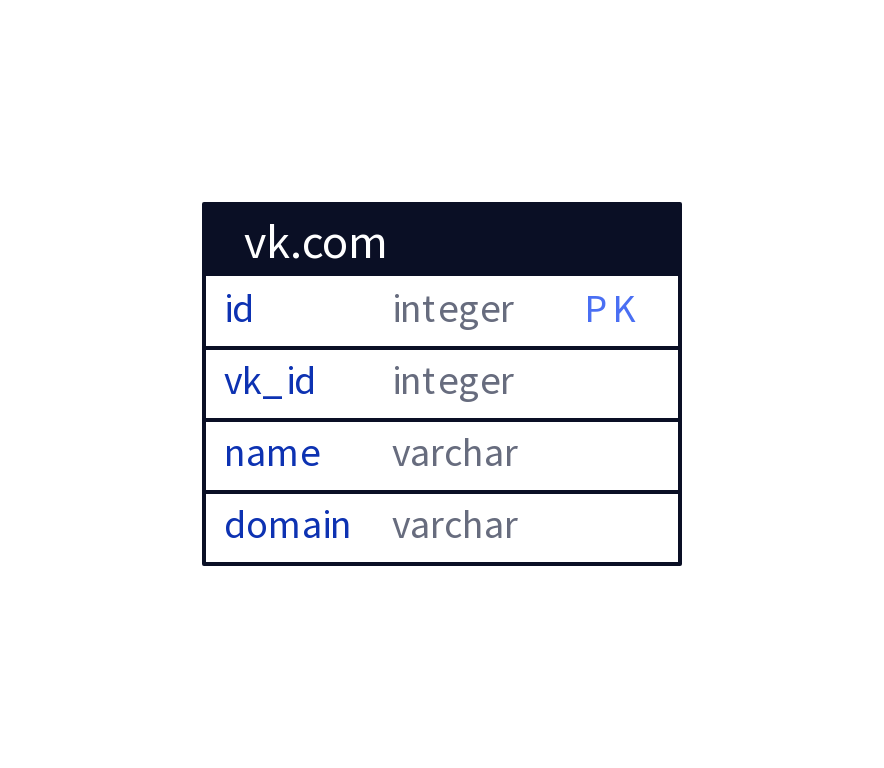
\includegraphics[width=0.8\textwidth]{img/d2/vk_com.png}
\caption{\label{fig:database_vk_com}Схема базы данных сайта vk.com}
\end{figure}

\chapter{Запросы API}
\label{sec:org54fd70e}
\begin{longtblr}[caption={Запросы API\label{tbl:api_doc} }]{colspec={|X[l]|X[l]|X[l]|X[l]|},rowhead = 1,hlines}
\textbf{Путь}&\textbf{Параметры запроса}&\textbf{Тело запроса}&\textbf{Результат запроса}\\\par
GET\par/text/sentences&sources: array\par
model\_id: integer\par
limit: integer&&\{\par
	items: [\{\par
	sentence\_id: integer\par
	sentence: string\par
\}]\par
\}\\\par
POST\par/text/&&\{\par
	items: [\{\par
	source\_id: integer\par
	date: string\par
	title: string\par
	text: string\par
	bank\_id: integer\par
	link: string\par
	comments\_num: integer\par
\}]\par
	parser\_state: string\par
	date: string\par
\}&\\\par
GET\par/model/&&&\{\par
	items: [\{\par
	id: integer\par
	name: string\par
	model\_type\_id: integer\par
	model\_type: string\par
\}]\par
\}\\\par
POST\par/model/&&\{\par
	model\_name: string\par
	model\_type: string\par
\}&\{\par
	model\_id: integer\par
\}\\\par
GET\par/model/type/&&&\{\par
	items: [\{\par
	id: integer\par
	model\_type: string\par
\}]\par
\}\\\par
GET\par/text\_result/item/\{text\_id\}&text\_id: integer&&\{\par
	items: [\{\par
	id: integer\par
	text\_sentence\_id: integer\par
	result: array[number]\par
	model\_id: integer\par
\}]\par
\}\\\par
POST\par/text\_result/&&\{\par
	items: [\{\par
	text\_result: array[number]\par
	model\_id: integer\par
	text\_sentence\_id: integer\par
\}]\par
\}&\\\par
GET\par/source/&&&\{\par
	items: [\{\par
	id: integer\par
	site: string\par
	source\_type\_id: integer\par
	parser\_state: string\par
	last\_update: string\par
\}]\par
\}\\\par
POST\par/source/&&\{\par
	site: string\par
	source\_type: string\par
\}&\{\par
	id: integer\par
	site: string\par
	source\_type\_id: integer\par
	parser\_state: string\par
	last\_update: string\par
\}\\\par
GET\par/source/item/\{source\_id\}&source\_id: integer&&\{\par
	id: integer\par
	site: string\par
	source\_type\_id: integer\par
	parser\_state: string\par
	last\_update: string\par
\}\\\par
PATCH\par/source/item/\{source\_id\}&source\_id: integer&\{\par
	parser\_state: string\par
	last\_update: string\par
\}&\{\par
	id: integer\par
	site: string\par
	source\_type\_id: integer\par
	parser\_state: string\par
	last\_update: string\par
\}\\\par
GET\par/source/type/&&&\{\par
	items: [\{\par
	id: integer\par
	name: string\par
\}]\par
\}\\\par
GET\par/bank/&&&\{\par
	items: [\{\par
	id: integer\par
	bank\_name: string\par
	licence: string\par
	description: string\par
\}]\par
\}\\\par
GET\par/bank/broker&&&\{\par
	items: [\{\par
	id: integer\par
	bank\_name: string\par
	licence: string\par
	description: string\par
\}]\par
\}\\\par
GET\par/bank/insurance&&&\{\par
	items: [\{\par
	id: integer\par
	bank\_name: string\par
	licence: string\par
	description: string\par
\}]\par
\}\\\par
GET\par/bank/mfo&&&\{\par
	items: [\{\par
	id: integer\par
	bank\_name: string\par
	licence: string\par
	description: string\par
\}]\par
\}\\\par
GET\par/views/aggregate\_text\_result&start\_year: integer\par
end\_year: integer\par
bank\_ids: array\par
model\_names: array\par
source\_type: array\par
aggregate\_by\_year: boolean\par
index\_type: None&&\{\par
	items: [\{\par
	year: integer\par
	quarter: integer\par
	date: string\par
	bank\_name: string\par
	bank\_id: integer\par
	model\_name: string\par
	source\_type: string\par
	index: number\par
	index\_10\_percentile: number\par
	index\_90\_percentile: number\par
\}]\par
\}\\\par
GET\par/views/reviews\_count&start\_date: string\par
end\_date: string\par
source\_sites: array\par
aggregate\_by: None&&\{\par
	items: [\{\par
	date: string\par
	source\_site: string\par
	source\_type: string\par
	count: integer\par
\}]\par
\}\\
\end{longtblr}


\begin{landscape}
\chapter{Диаграмма классов}
\label{sec:orge49e4c8}
\begin{figure}[h!]
\centering
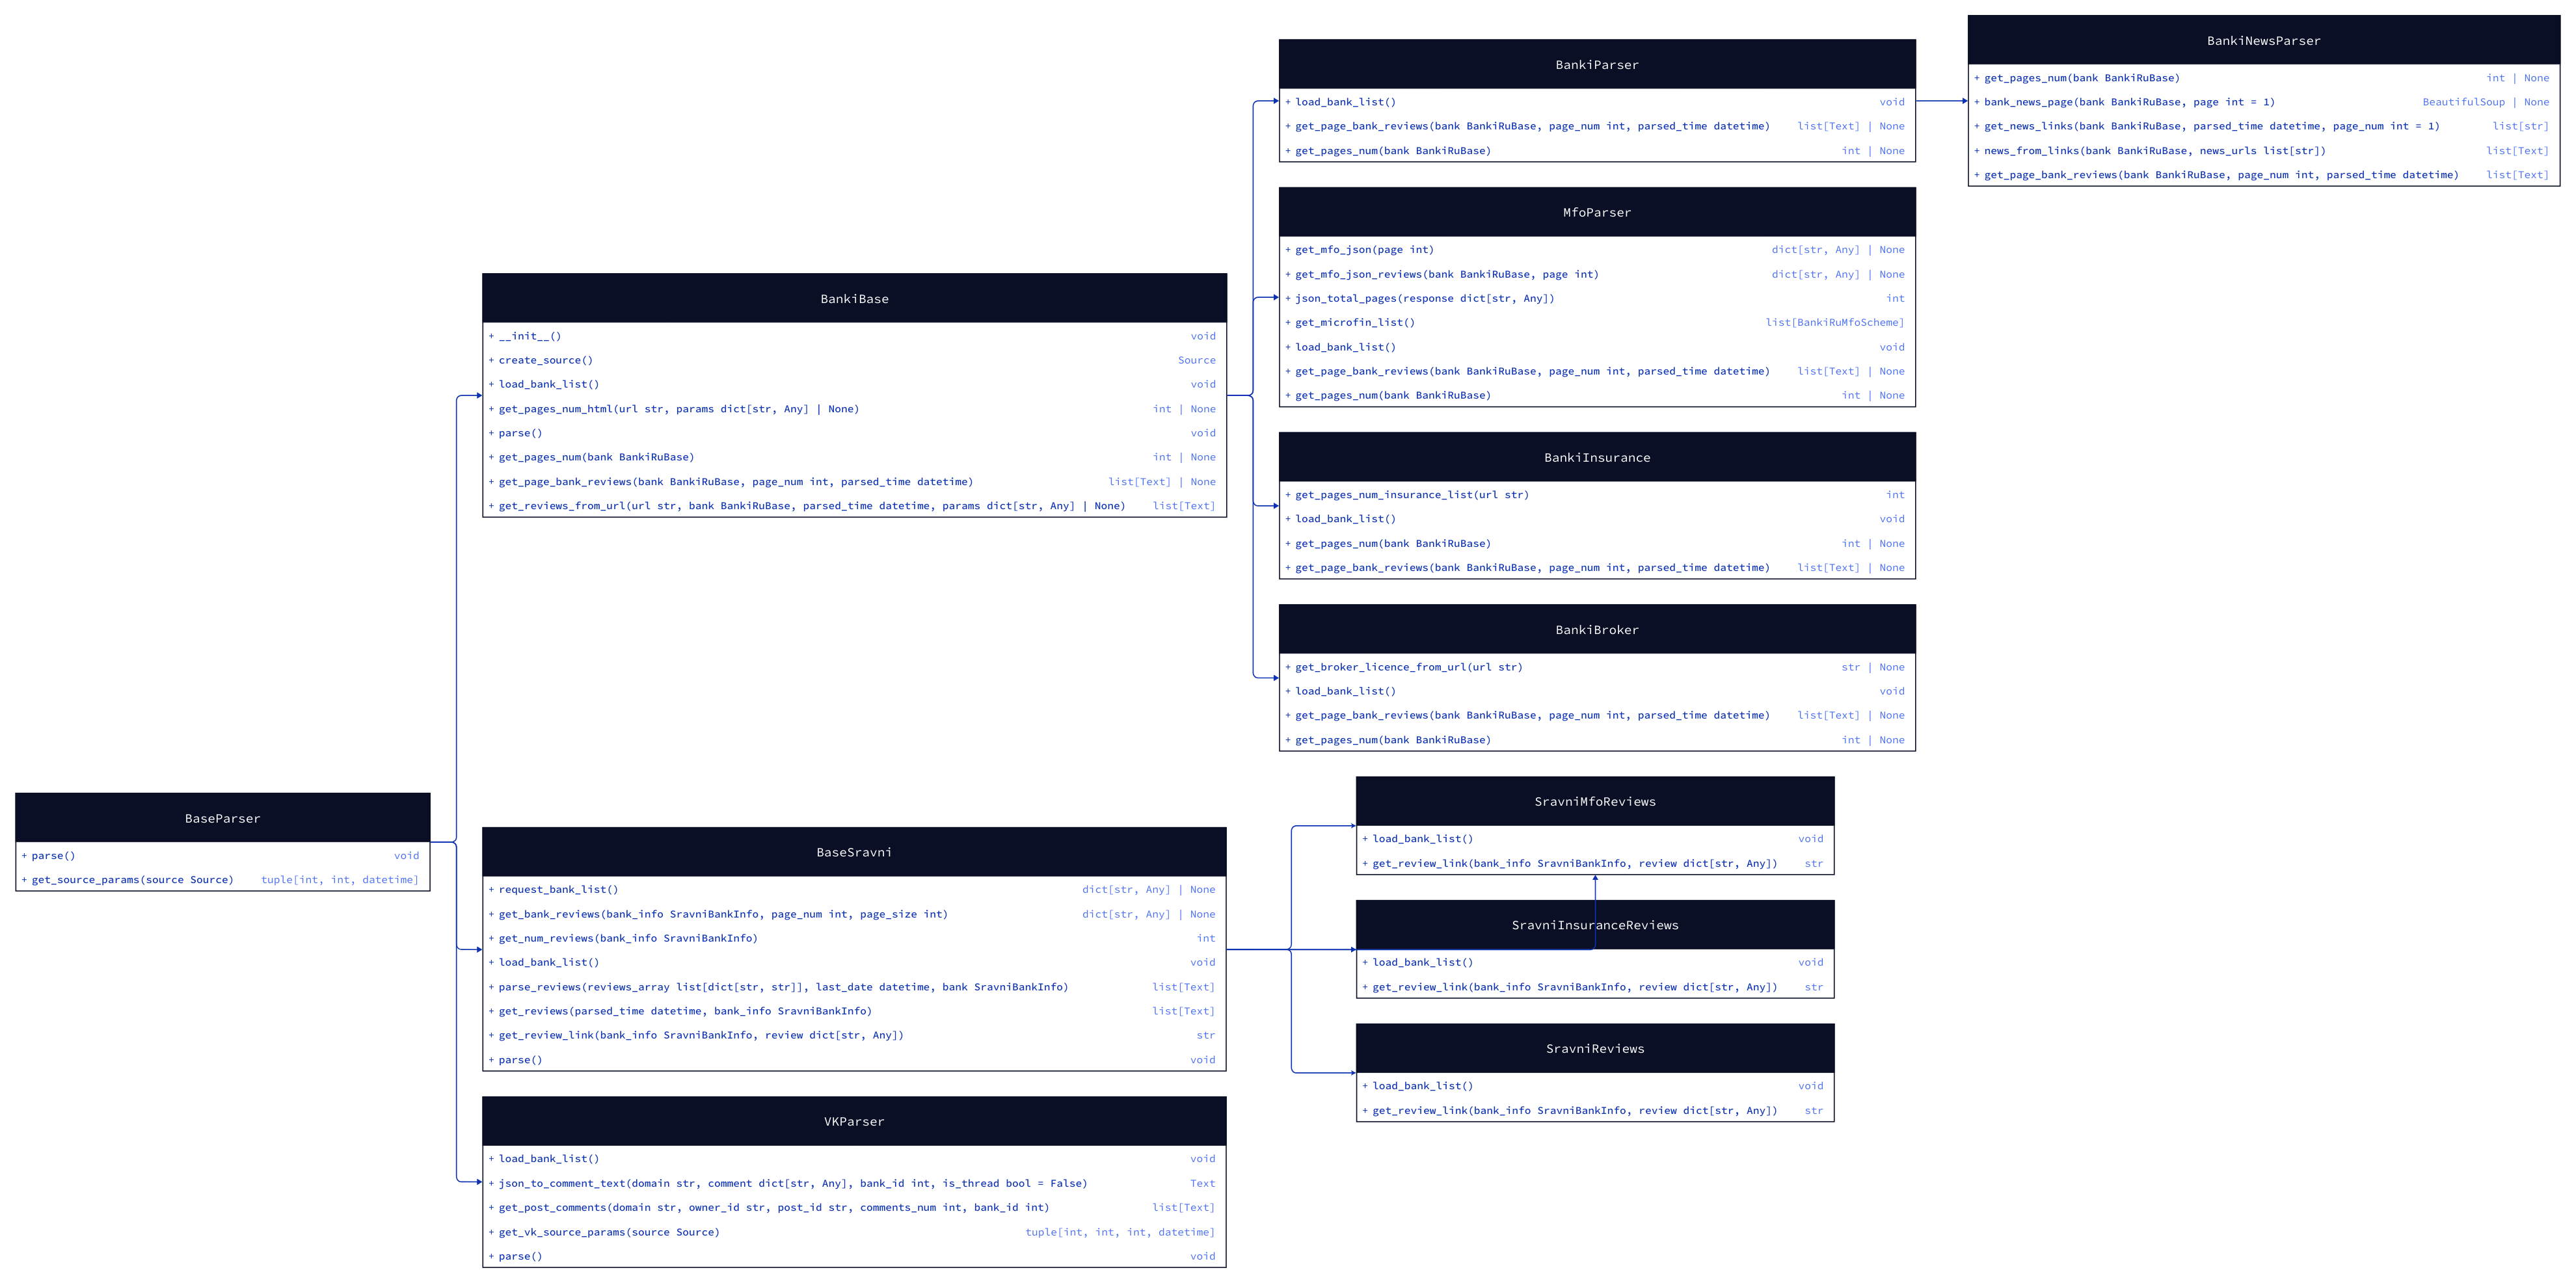
\includegraphics[width=.9\linewidth]{img/d2/parser_class.png}
\caption{\label{fig:parser_class_diagram}Схема классов сборщиков данных}
\end{figure}
\end{landscape}
\chapter{Листинг программы}
\label{sec:org5951735}
В данном документе представлено описание структуры репозитория, в котором находится исходный код системы, описанной и разработанной в работе.

Репозиторий программы находится по ссылке: \url{https://github.com/Samoed/EthicsAnalysis}.
\chapter{Акт о внедрении}
\label{sec:orge719756}
\hspace*{-2cm}
\includegraphics[scale=0.85]{img/deployment_act.pdf}
\end{document}
